\chapter{Hyperbolic geometry}
\label{chap:hyperbolic_geometry}
\section{Basic facts}
Hyperbolic geometry, sometimes called Lobachevskian geometry\footnote{After the Russian mathematician Nikolai Lobachevsky (1832) who first published about this subject \cite{Needham1997}.} is the geometry on the hyperbolic plane. This type of geometry is called non-Euclidean, because it does not satisfy all of Euclid's axioms that form the building blocks of traditional  geometry. More specifically, the fifth axiom, called the parallel axiom, states that \cite{Needham1997}
\begin{quote}
    Through any point \(p\) not on the line \(L\) there exists precisely one line \(L'\) that does not meet \(L\).
\end{quote}
Logic dictates that if this axiom is not true, two possible alternatives arise. Given again the point \(p\) and the line \(L\), 
\begin{itemize}
    \item there exists \emph{no} line through \(p\) that does not meet \(L\), or
    \item there exist \emph{at least two} lines through \(p\) that do not meet \(L\).
\end{itemize}
The first statement corresponds to what is called \emph{spherical geometry}, while the latter is the defining axiom for \emph{hyperbolic geometry}. It does not take too much imagination to realize that the parallel axiom is equivalent to another basic fact in Euclidean geometry: the sum of the angles of a triangle is equal to \(\pi\). As such, for both types of non-Euclidean geometry this will not be the case; let \(\mathcal{E}(T)\) denote the \emph{angular excess} of a triangle \(T\) in a certain geometry.
\begin{itemize}
    \item Naturally, for Euclidean geometry \(\mathcal{E}(T) = 0\),
    \item in spherical geometry, \(\mathcal{E}(T) > 0\),
    \item in hyperbolic geometry, \(\mathcal{E}(T) < 0\).
\end{itemize}
It may come as a surprise that the angular excess can be related to the size of the triangle (more specifically, its area) like so \cite{Needham1997}
\begin{equation}
    \mathcal{E}(T) = k\mathcal{A}(T)
    \label{eq:angular_excess} 
\end{equation}
where \(k = 0\) for Euclidean geometry, \(k < 0\) for hyperbolic geometry and \(k > 0\) for spherical geometry. This hints at the fact that spherical geometry and hyperbolic geometry are somehow `larger' classes of geometry than Euclidean geometry, since they exist for a whole range of values for \(k\), be it positive or negative. There is indeed a `different' geometry for every value of \(k\), and only one of those values corresponds to the traditional concept of Euclidean geometry that most people are familiar with. Another consequence of \cref{eq:angular_excess} is that similar triangles cannot exist in non-Euclidean geometry; since apart from the trivial case where the triangles are also congruent, they must differ in area, which yields a different angular excess. The value of \(k\) is, as it turns out, equal to the \emph{Gaussian curvature} of the surface: a negatively curved surface has an angular deficiency while a positively curved surface has an angular excess; only for surface with zero curvature the sum of the angles of a triangle will be precisely equal to \(\pic\).

\subsection{Surface curvature}
Perhaps one of the most remarkable results attributed to Carl Friedrich Gauss is his \emph{Theorema Egregium} about the (Gaussian) curvature of surfaces. The theorem states that curvature is an \emph{intrinsic} property, which means that it remains preserved when the surface is transformed by `bending without stretching'. Curvature can be positive, negative or zero. Positively curved surfaces `bend away' from their tangent plane in any direction (local convexity) and negatively curved surfaces intersect their tangent plane like a saddle. For surfaces with zero curvature, there is always at least one straight line that lies in the tangent plane; examples are a cylinder (always one straight line) and a plane (straight lines in two directions). If a coordinate system is defined such that the point at issue is at the origin and the tangent plane to the surface described by \(f(x, y)\) coincides with the horizontal, the Gaussian curvature can be computed by means of the determinant of the Hessian \cite{Thurston1997, ONeill2006}
    \[ 
        k = \det \begin{pmatrix}
                f_{xx} & f_{xy}\\
                f_{yx} & f_{yy}
        \end{pmatrix}.
    \]
    Surface curvature can be approached more rigorously from the perspective of Riemannian geometry. The core concept behind Riemannian geometry are the eponymous manifolds: these are manifolds equipped with an positive definite inner product\footnote{In contrast to \cref{sec:lorentz_metric}, the positive definiteness of the inner product is essential for Riemannian geometry. When the inner product is not positive definite but nondegenerate, as the Lorentz product, the manifold is called \emph{pseudo-Riemannian}.} on their tangent space, hence providing a \emph{metric (tensor)} that allows to determine lengths, angles and curvature. The metric on a parametric surface \(\vb{r}(u, v)\) can be written in terms of the so-called \emph{first fundamental form} I, which is defined as the inner product of two tangent vectors to the surface  and is characterised by coefficients \(E\), \(F\) and \(G\).
\begin{equation}
    \begin{split}
        E &= \vb{r}_u \cdot \vb{r}_u \\
        F &= \vb{r}_u \cdot \vb{r}_v \\
        G &= \vb{r}_v \cdot \vb{r}_v \\
        \text{with }  \vb{r}_u = & \pdv{\vb{r}}{u},\ \vb{r}_v = \pdv{\vb{r}}{v}.
    \end{split}
    \label{eq:first_fform}
\end{equation}
The components of the metric tensor \(\mathtens{g}_{ij}\) then coincide with the components of the first fundamental form: \(\mathtens{g}_{11} = E\), \(\mathtens{g}_{12} = \mathtens{g}_{21}= F\) and \(\mathtens{g}_{22} = G\). Therefore, the first fundamental form determines the length of curves lying in the surface.

In contrast, the \emph{second fundamental form} II provides information on the curvature or shape of the embedded surface, more specifically the rate of change of the tangent planes in any direction. Again, it is characterised by three coefficients \(e\), \(f\) and \(g\) like so 
\[ e\dd{u}^2 + 2f\dd{u}\dd{v} + g\dd{v}^2. \]
The coefficients of the second fundamental form can be computed using the surface unit normal vector 
\[
    \vb{n} =  \frac{\vb{r}_u \cross \vb{r}_v}{\norm{\vb{r}_u \cross \vb{r}_v}},
\]
the coefficients are then given by
\begin{equation}
    \begin{split}
        e &= \vb{r}_{uu} \cdot \vb{n} = -\sech(u)\tanh(u)\\
        f &= \vb{r}_{uv} \cdot \vb{n} = 0\\
        g &= \vb{r}_{vv} \cdot \vb{n} = \sech(u)\tanh(u)\\
        \text{with }\ & \vb{r}_{uu} = \pdv[2]{\vb{r}}{u}\ \text{ etc.}
    \end{split}
    \label{eq:second_fform}
\end{equation}


\subsection{The pseudosphere}
Pseudospherical surfaces are surfaces of constant negative curvature, in that sense exhibiting a certain duality to a sphere which is a surface of constant positive curvature. The most notable example is the \emph{pseudosphere}; which is the surface of revolution of a tractrix --- another name for the pseudosphere is a \emph{tractricoid}. A tractrix is a curve defined by the property that the segment of the tangent from the point to the axis has constant length \(R\). It can be parameterized by the pair

\towrite{derivation tractrix}

    \[ 
        \qty(R(t - \tanh(t)),\ R\cosh[-1](t)) \quad t \in \real^+.
    \]
It can be shown that this surface has a constant curvature of \(1/R^2\)
\begin{figure}[ht]
    \begin{subfigure}[b]{0.5\textwidth}
        \centering
        \begin{tikzpicture}[scale=3]
    \draw[->] (0, -0.2) -- (0, 2);
    \draw[->] (-0.2, 0) -- (1.2, 0);
    \draw[domain=0:2.8, smooth, variable=\t, thick] plot ({1/cosh(\t)}, {\t - tanh(\t)});
    
    \foreach \t in {0.35, 0.8, 1.3} {
        \filldraw[dashed] ({1/cosh(\t)}, {\t - tanh(\t)}) circle (0.4pt)
        -- (0,  {\t - tanh(\t) + sqrt(1 - (1/cosh(\t))^2)}) circle (0.4pt) node[pos=0.7, fill=white] {$_R$};
    }

\end{tikzpicture}
        \caption{The tractrix - the line segments defined on the tangent to the curve between the curve and the intersection with the vertical axis all have the same length \(R\).}
        \label{fig:tractrix}
    \end{subfigure}
    \begin{subfigure}[b]{0.45\textwidth}
        \centering
        % This file was created by matlab2tikz.
%
%The latest updates can be retrieved from
%  http://www.mathworks.com/matlabcentral/fileexchange/22022-matlab2tikz-matlab2tikz
%where you can also make suggestions and rate matlab2tikz.
%
\definecolor{mycolor1}{rgb}{0.00000,0.44700,0.74100}%
%
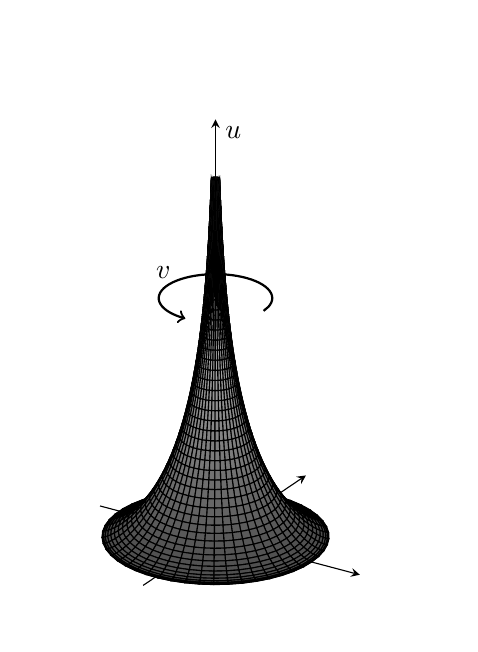
\begin{tikzpicture}[scale=1]

\begin{axis}[%
    width=2.113in,
    height=2.98in,
    at={(1.59in,0.402in)},
    scale only axis,
    plot box ratio=1 1.001 1.502,
    axis lines = middle,
    xmin=-1.2,
    xmax=1.5,
    ticks=none,
    ymin=-1.2,
    ymax=1.5,
    zmin=0,
    zmax=3.5,
    zlabel=\(u\),
    view={32.0545132396862}{25.0188534547135},
    axis background/.style={fill=white},
]
    \addplot3[domain=0:50, ->, thick]
    table[row sep=crcr] {
        0.5  0.0  2\\
        0.49077957849553266  0.09557931435068615  2\\
        0.4793339265183303  0.1422637933155162  2\\
        0.4634583786730109  0.18763350243968704  2\\
        0.44329965318650005  0.23126914512041763  2\\
        0.41904405244592036  0.2727674506052743  2\\
        0.3909157412340149  0.31174490092936674  2\\
        0.35917467504886386  0.3478412753017432  2\\
        0.32411419765389426  0.38072297918456716  2\\
        0.28605833006108483  0.41008612729847793  2\\
        0.24535877600196895  0.4356593520616947  2\\
        0.202391671561197  0.4572063115079062  2\\
        0.15755410901181038  0.4745278735053343  2\\
        0.11126046697815722  0.4874639560909118  2\\
        0.06393858084225311  0.495895006911623  2\\
        0.016025788785827666  0.49974310810034395  2\\
        -0.032035109990356414  0.49897269637516817  2\\
        -0.07979994751668948  0.4935908917072251  2\\
        -0.1268272919547536  0.4836474315195147  2\\
        -0.17268252721065375  0.4692342110248802  2\\
        -0.21694186955877903  0.4504844339512096  2\\
        -0.2591962841552625  0.4275713815026731  2\\
        -0.2990552652456078  0.4007068109339785  2\\
        -0.3361504451306583  0.37013899853765786  2\\
        -0.3701389985376577  0.3361504451306585  2\\
        -0.40070681093397825  0.29905526524560805  2\\
        -0.42757138150267304  0.2591962841552626  2\\
        -0.4504844339512095  0.21694186955877912  2\\
        -0.4692342110248801  0.17268252721065405  2\\
        -0.48364743151951467  0.1268272919547539  2\\
        -0.49359089170722503  0.0797999475166898  2\\
        -0.49897269637516817  0.032035109990356615  2\\
        -0.49974310810034395  -0.01602578878582746  2\\
        -0.4958950069116231  -0.06393858084225292  2\\
        -0.4874639560909118  -0.11126046697815714  2\\
        -0.47452787350533443  -0.1575541090118101  2\\
        -0.45720631150790636  -0.2023916715611967  2\\
        -0.43565935206169476  -0.24535877600196876  2\\
        -0.41008612729847804  -0.28605833006108466  2\\
        -0.3807229791845673  -0.3241141976538941  2\\
        -0.34784127530174325  -0.3591746750488637  2\\
        -0.31174490092936685  -0.39091574123401485  2\\
        -0.2727674506052746  -0.4190440524459202  2\\
        -0.23126914512041766  -0.4432996531865  2\\
        -0.18763350243968727  -0.4634583786730108  2\\
        -0.1422637933155166  -0.4793339265183302  2\\
        -0.0955793143506863  -0.49077957849553266  2\\
        -0.04801151295384122  -0.49768955647459906  2\\
        -9.184850993605148e-17  -0.5  2\\
    } node[pos=0.7, above] {\(v\)};

    \addplot3 [color=mycolor1]
     table[row sep=crcr] {%
    1	0	0\\
    0.996677281521151	0	0.000180848295413094\\
    0.986818657254952	0	0.00143534074664706\\
    0.970744026930539	0	0.00478124968872615\\
    0.948958838413527	0	0.0111306709055737\\
    0.922116636293008	0	0.021251248082997\\
    0.890973941781643	0	0.0357414777260489\\
    0.856342883234364	0	0.0550209162433916\\
    0.819046488706006	0	0.0793340686584179\\
    0.779880351526415	0	0.108765257576638\\
    0.739582863872753	0	0.143261015624456\\
    0.698814736566502	0	0.182656475753605\\
    0.658147333570727	0	0.226702676689377\\
    0.618058560319707	0	0.275092429633295\\
    0.578934654256853	0	0.327483200361739\\
    0.541076158953017	0	0.383516199297968\\
    0.504706515831052	0	0.4428314592909\\
    0.469981979037802	0	0.505079091615864\\
    0.437001869679927	0	0.569927157912677\\
    0.405818482253955	0	0.637066711600307\\
    0.376446209482368	0	0.70621458438625\\
    0.348869650868407	0	0.777114456348854\\
    0.323050615738523	0	0.849536679194129\\
    0.298934030278091	0	0.923277241274682\\
    0.276452819459861	0	0.998156182388777\\
    0.255531868277275	0	1.07401569336226\\
    0.236091180639736	0	1.15071807320667\\
    0.218048355357848	0	1.22814366601495\\
    0.201320491892778	0	1.30618886003915\\
    0.185825627569285	0	1.38476420122183\\
    0.171483795196121	0	1.46379265120814\\
    0.158217777058867	0	1.54320800395986\\
    0.145953618972422	0	1.62295346409914\\
    0.134620956991128	0	1.70298038282444\\
    0.124153199675171	0	1.78324714268591\\
    0.114487600525916	0	1.86371817991473\\
    0.10556524825076	0	1.94436313178065\\
    0.0973309967677409	0	2.02515609616461\\
    0.0897333521584377	0	2.10607499085338\\
    0.0827243299703536	0	2.18710100075792\\
    0.0762592932121512	0	2.26821810216251\\
    0.0702967789469859	0	2.34941265411304\\
    0.0647983194579305	0	2.43067304807599\\
    0.0597282624391434	0	2.51198940799476\\
    0.055053593476748	0	2.59335333380767\\
    0.0507437631581477	0	2.67475768235632\\
    0.0467705204335336	0	2.7561963803967\\
    0.0431077533047957	0	2.8376642651264\\
    0.039731337499592	0	2.91915694826365\\
    0.0366189934736865	0	3.00067070026093\\
    };
     
    \addplot3[%
    surf,
    shader=flat corner, draw=black, z buffer=sort, colormap={mymap}{[1pt] rgb(0pt)=(0.3,0.3,0.3); rgb(255pt)=(1,1,1)}, mesh/rows=50]
    table[row sep=crcr, point meta=\thisrow{c}] {%
    %
    x	y	z	c\\
    1	0	0	0\\
    0.991790013823246	0.127877161684506	0	0\\
    0.967294863039029	0.253654583909507	0	0\\
    0.926916757346022	0.375267004879374	0	0\\
    0.871318704123389	0.490717552003938	0	0\\
    0.801413621867957	0.598110530491216	0	0\\
    0.718349350097728	0.695682550603486	0	0\\
    0.623489801858734	0.78183148246803	0	0\\
    0.518392568310525	0.855142763005346	0	0\\
    0.404783343122394	0.914412623015812	0	0\\
    0.284527586631032	0.958667853036661	0	0\\
    0.15959989503338	0.98718178341445	0	0\\
    0.0320515775716553	0.999486216200688	0	0\\
    -0.0960230259076818	0.995379112949198	0	0\\
    -0.222520933956314	0.974927912181824	0	0\\
    -0.345365054421307	0.93846842204976	0	0\\
    -0.462538290240835	0.886599306373	0	0\\
    -0.57211666012217	0.820172254596956	0	0\\
    -0.672300890261317	0.740277997075315	0	0\\
    -0.761445958369134	0.648228395307789	0	0\\
    -0.838088104891841	0.545534901210549	0	0\\
    -0.900968867902419	0.433883739117558	0	0\\
    -0.949055747010669	0.315108218023621	0	0\\
    -0.981559156991065	0.191158628701373	0	0\\
    -0.997945392750336	0.0640702199807132	0	0\\
    -0.997945392750336	-0.064070219980713	0	0\\
    -0.981559156991065	-0.191158628701372	0	0\\
    -0.949055747010669	-0.315108218023621	0	0\\
    -0.900968867902419	-0.433883739117558	0	0\\
    -0.838088104891841	-0.545534901210548	0	0\\
    -0.761445958369135	-0.648228395307788	0	0\\
    -0.672300890261317	-0.740277997075315	0	0\\
    -0.57211666012217	-0.820172254596956	0	0\\
    -0.462538290240835	-0.886599306373	0	0\\
    -0.345365054421307	-0.938468422049761	0	0\\
    -0.222520933956315	-0.974927912181824	0	0\\
    -0.0960230259076816	-0.995379112949198	0	0\\
    0.0320515775716549	-0.999486216200688	0	0\\
    0.159599895033378	-0.98718178341445	0	0\\
    0.284527586631032	-0.958667853036661	0	0\\
    0.404783343122394	-0.914412623015812	0	0\\
    0.518392568310524	-0.855142763005346	0	0\\
    0.623489801858733	-0.78183148246803	0	0\\
    0.718349350097727	-0.695682550603487	0	0\\
    0.801413621867956	-0.598110530491217	0	0\\
    0.871318704123389	-0.490717552003938	0	0\\
    0.926916757346022	-0.375267004879375	0	0\\
    0.967294863039029	-0.253654583909508	0	0\\
    0.991790013823246	-0.127877161684507	0	0\\
    1	-2.44929359829471e-16	0	0\\
    0.996677281521151	0	0.000180848295413094	0.000180848295413094\\
    0.988494574817178	0.127452261876354	0.000180848295413094	0.000180848295413094\\
    0.964080814523114	0.252811761136307	0.000180848295413094	0.000180848295413094\\
    0.923836873908034	0.374020098267759	0.000180848295413094	0.000180848295413094\\
    0.868423557364232	0.489087035725999	0.000180848295413094	0.000180848295413094\\
    0.798750750017375	0.596123177579159	0.000180848295413094	0.000180848295413094\\
    0.715962477437889	0.693370993337184	0.000180848295413094	0.000180848295413094\\
    0.621418120772724	0.779233676553888	0.000180848295413094	0.000180848295413094\\
    0.516670095744502	0.852301364344654	0.000180848295413094	0.000180848295413094\\
    0.403438362028271	0.911374287296025	0.000180848295413094	0.000180848295413094\\
    0.283582181561191	0.955482469646297	0.000180848295413094	0.000180848295413094\\
    0.15906958951293	0.983901656260716	0.000180848295413094	0.000180848295413094\\
    0.0319450792025817	0.996165204880763	0.000180848295413094	0.000180848295413094\\
    -0.0957039684251033	0.992071748377142	0.000180848295413094	0.000180848295413094\\
    -0.221781559537127	0.971688501192472	0.000180848295413094	0.000180848295413094\\
    -0.344217503573033	0.935350155682	0.000180848295413094	0.000180848295413094\\
    -0.461001405716677	0.88365338647438	0.000180848295413094	0.000180848295413094\\
    -0.570215677523525	0.817447053090767	0.000180848295413094	0.000180848295413094\\
    -0.670067023669899	0.737818261694948	0.000180848295413094	0.000180848295413094\\
    -0.758915887812616	0.646074514840185	0.000180848295413094	0.000180848295413094\\
    -0.835303374058813	0.543722242313439	0.000180848295413094	0.000180848295413094\\
    -0.897975201996172	0.43244206559992	0.000180848295413094	0.000180848295413094\\
    -0.945902301942619	0.314061202124757	0.000180848295413094	0.000180848295413094\\
    -0.978297712242048	0.190523462393395	0.000180848295413094	0.000180848295413094\\
    -0.994629501152963	0.0638573326768394	0.000180848295413094	0.000180848295413094\\
    -0.994629501152963	-0.0638573326768392	0.000180848295413094	0.000180848295413094\\
    -0.978297712242048	-0.190523462393395	0.000180848295413094	0.000180848295413094\\
    -0.945902301942619	-0.314061202124756	0.000180848295413094	0.000180848295413094\\
    -0.897975201996172	-0.43244206559992	0.000180848295413094	0.000180848295413094\\
    -0.835303374058813	-0.543722242313439	0.000180848295413094	0.000180848295413094\\
    -0.758915887812617	-0.646074514840185	0.000180848295413094	0.000180848295413094\\
    -0.670067023669899	-0.737818261694948	0.000180848295413094	0.000180848295413094\\
    -0.570215677523525	-0.817447053090767	0.000180848295413094	0.000180848295413094\\
    -0.461001405716677	-0.88365338647438	0.000180848295413094	0.000180848295413094\\
    -0.344217503573033	-0.935350155682	0.000180848295413094	0.000180848295413094\\
    -0.221781559537127	-0.971688501192472	0.000180848295413094	0.000180848295413094\\
    -0.0957039684251031	-0.992071748377142	0.000180848295413094	0.000180848295413094\\
    0.0319450792025813	-0.996165204880763	0.000180848295413094	0.000180848295413094\\
    0.159069589512929	-0.983901656260716	0.000180848295413094	0.000180848295413094\\
    0.283582181561191	-0.955482469646298	0.000180848295413094	0.000180848295413094\\
    0.403438362028271	-0.911374287296025	0.000180848295413094	0.000180848295413094\\
    0.516670095744501	-0.852301364344655	0.000180848295413094	0.000180848295413094\\
    0.621418120772724	-0.779233676553888	0.000180848295413094	0.000180848295413094\\
    0.715962477437888	-0.693370993337184	0.000180848295413094	0.000180848295413094\\
    0.798750750017374	-0.59612317757916	0.000180848295413094	0.000180848295413094\\
    0.868423557364232	-0.489087035725999	0.000180848295413094	0.000180848295413094\\
    0.923836873908033	-0.37402009826776	0.000180848295413094	0.000180848295413094\\
    0.964080814523114	-0.252811761136307	0.000180848295413094	0.000180848295413094\\
    0.988494574817178	-0.127452261876355	0.000180848295413094	0.000180848295413094\\
    0.996677281521151	-2.44115528519553e-16	0.000180848295413094	0.000180848295413094\\
    0.986818657254952	0	0.00143534074664706	0.00143534074664706\\
    0.978716889719926	0.126191568987079	0.00143534074664706	0.00143534074664706\\
    0.954544617913788	0.250311075900144	0.00143534074664706	0.00143534074664706\\
    0.914698749871315	0.370320481867152	0.00143534074664706	0.00143534074664706\\
    0.859833553644168	0.484249235759963	0.00143534074664706	0.00143534074664706\\
    0.790849914237565	0.590226630589389	0.00143534074664706	0.00143534074664706\\
    0.708880541103407	0.686512520462233	0.00143534074664706	0.00143534074664706\\
    0.615271369082392	0.77152589372875	0.00143534074664706	0.00143534074664706\\
    0.511559458191139	0.843870833150225	0.00143534074664706	0.00143534074664706\\
    0.399447755139211	0.902359436821443	0.00143534074664706	0.00143534074664706\\
    0.280777130991228	0.946031323487125	0.00143534074664706	0.00143534074664706\\
    0.157496154114871	0.974169401975597	0.00143534074664706	0.00143534074664706\\
    0.0316290947421639	0.986311645815996	0.00143534074664706	0.00143534074664706\\
    -0.094757313491776	0.982258679700153	0.00143534074664706	0.00143534074664706\\
    -0.219587809257888	0.962077053219641	0.00143534074664706	0.00143534074664706\\
    -0.340812679266818	0.926098148123318	0.00143534074664706	0.00143534074664706\\
    -0.456441414504462	0.874912737038176	0.00143534074664706	0.00143534074664706\\
    -0.564575394334947	0.809361282999135	0.00143534074664706	0.00143534074664706\\
    -0.663439061798982	0.730520139069248	0.00143534074664706	0.00143534074664706\\
    -0.751409078210039	0.639683874652164	0.00143534074664706	0.00143534074664706\\
    -0.827040978330714	0.538344018698307	0.00143534074664706	0.00143534074664706\\
    -0.88909288845198	0.428164568840747	0.00143534074664706	0.00143534074664706\\
    -0.936545917925164	0.310954668600071	0.00143534074664706	0.00143534074664706\\
    -0.968620889318226	0.188638901297786	0.00143534074664706	0.00143534074664706\\
    -0.984791132487653	0.0632256884513968	0.00143534074664706	0.00143534074664706\\
    -0.984791132487653	-0.0632256884513966	0.00143534074664706	0.00143534074664706\\
    -0.968620889318226	-0.188638901297786	0.00143534074664706	0.00143534074664706\\
    -0.936545917925164	-0.31095466860007	0.00143534074664706	0.00143534074664706\\
    -0.88909288845198	-0.428164568840747	0.00143534074664706	0.00143534074664706\\
    -0.827040978330714	-0.538344018698307	0.00143534074664706	0.00143534074664706\\
    -0.75140907821004	-0.639683874652164	0.00143534074664706	0.00143534074664706\\
    -0.663439061798982	-0.730520139069248	0.00143534074664706	0.00143534074664706\\
    -0.564575394334948	-0.809361282999135	0.00143534074664706	0.00143534074664706\\
    -0.456441414504462	-0.874912737038176	0.00143534074664706	0.00143534074664706\\
    -0.340812679266818	-0.926098148123318	0.00143534074664706	0.00143534074664706\\
    -0.219587809257888	-0.962077053219641	0.00143534074664706	0.00143534074664706\\
    -0.0947573134917758	-0.982258679700153	0.00143534074664706	0.00143534074664706\\
    0.0316290947421634	-0.986311645815996	0.00143534074664706	0.00143534074664706\\
    0.15749615411487	-0.974169401975597	0.00143534074664706	0.00143534074664706\\
    0.280777130991227	-0.946031323487125	0.00143534074664706	0.00143534074664706\\
    0.399447755139211	-0.902359436821443	0.00143534074664706	0.00143534074664706\\
    0.511559458191138	-0.843870833150226	0.00143534074664706	0.00143534074664706\\
    0.615271369082391	-0.77152589372875	0.00143534074664706	0.00143534074664706\\
    0.708880541103407	-0.686512520462233	0.00143534074664706	0.00143534074664706\\
    0.790849914237564	-0.59022663058939	0.00143534074664706	0.00143534074664706\\
    0.859833553644168	-0.484249235759963	0.00143534074664706	0.00143534074664706\\
    0.914698749871315	-0.370320481867152	0.00143534074664706	0.00143534074664706\\
    0.954544617913788	-0.250311075900144	0.00143534074664706	0.00143534074664706\\
    0.978716889719926	-0.126191568987079	0.00143534074664706	0.00143534074664706\\
    0.986818657254952	-2.41700861989233e-16	0.00143534074664706	0.00143534074664706\\
    0.970744026930539	0	0.00478124968872615	0.00478124968872615\\
    0.962774231888273	0.124135990886065	0.00478124968872615	0.00478124968872615\\
    0.938995710575732	0.246233672233705	0.00478124968872615	0.00478124968872615\\
    0.899798905655474	0.364288203490766	0.00478124968872615	0.00478124968872615\\
    0.845827427580638	0.476361132517799	0.00478124968872615	0.00478124968872615\\
    0.777967486529088	0.580612224918604	0.00478124968872615	0.00478124968872615\\
    0.697333340856804	0.675329680638137	0.00478124968872615	0.00478124968872615\\
    0.605249001006471	0.758958241672088	0.00478124968872615	0.00478124968872615\\
    0.503226489292624	0.830124729360317	0.00478124968872615	0.00478124968872615\\
    0.392941012537039	0.887660591942487	0.00478124968872615	0.00478124968872615\\
    0.276203455219036	0.930621092145662	0.00478124968872615	0.00478124968872615\\
    0.154930644802394	0.958300819744214	0.00478124968872615	0.00478124968872615\\
    0.0311138774813852	0.970245274376223	0.00478124968872615	0.00478124968872615\\
    -0.0932137788476785	0.966258328426852	0.00478124968872615	0.00478124968872615\\
    -0.216010867505097	0.946405447438366	0.00478124968872615	0.00478124968872615\\
    -0.335261063690025	0.911012615167733	0.00478124968872615	0.00478124968872615\\
    -0.449006282477955	0.860660980942349	0.00478124968872615	0.00478124968872615\\
    -0.555378830521046	0.796177317204148	0.00478124968872615	0.00478124968872615\\
    -0.652632073521257	0.718620443928966	0.00478124968872615	0.00478124968872615\\
    -0.739169115917237	0.629263842831804	0.00478124968872615	0.00478124968872615\\
    -0.813569021865289	0.529574746832282	0.00478124968872615	0.00478124968872615\\
    -0.874610146966643	0.421190048130658	0.00478124968872615	0.00478124968872615\\
    -0.921290197634707	0.305889420483156	0.00478124968872615	0.00478124968872615\\
    -0.952842688728052	0.18556609700809	0.00478124968872615	0.00478124968872615\\
    -0.96874952921524	0.062195783350403	0.00478124968872615	0.00478124968872615\\
    -0.96874952921524	-0.0621957833504028	0.00478124968872615	0.00478124968872615\\
    -0.952842688728052	-0.18556609700809	0.00478124968872615	0.00478124968872615\\
    -0.921290197634707	-0.305889420483156	0.00478124968872615	0.00478124968872615\\
    -0.874610146966643	-0.421190048130658	0.00478124968872615	0.00478124968872615\\
    -0.813569021865289	-0.529574746832282	0.00478124968872615	0.00478124968872615\\
    -0.739169115917237	-0.629263842831804	0.00478124968872615	0.00478124968872615\\
    -0.652632073521257	-0.718620443928965	0.00478124968872615	0.00478124968872615\\
    -0.555378830521046	-0.796177317204148	0.00478124968872615	0.00478124968872615\\
    -0.449006282477955	-0.860660980942349	0.00478124968872615	0.00478124968872615\\
    -0.335261063690025	-0.911012615167733	0.00478124968872615	0.00478124968872615\\
    -0.216010867505097	-0.946405447438366	0.00478124968872615	0.00478124968872615\\
    -0.0932137788476783	-0.966258328426852	0.00478124968872615	0.00478124968872615\\
    0.0311138774813848	-0.970245274376223	0.00478124968872615	0.00478124968872615\\
    0.154930644802393	-0.958300819744215	0.00478124968872615	0.00478124968872615\\
    0.276203455219036	-0.930621092145662	0.00478124968872615	0.00478124968872615\\
    0.392941012537039	-0.887660591942487	0.00478124968872615	0.00478124968872615\\
    0.503226489292623	-0.830124729360317	0.00478124968872615	0.00478124968872615\\
    0.605249001006471	-0.758958241672088	0.00478124968872615	0.00478124968872615\\
    0.697333340856803	-0.675329680638137	0.00478124968872615	0.00478124968872615\\
    0.777967486529088	-0.580612224918605	0.00478124968872615	0.00478124968872615\\
    0.845827427580638	-0.476361132517799	0.00478124968872615	0.00478124968872615\\
    0.899798905655474	-0.364288203490766	0.00478124968872615	0.00478124968872615\\
    0.938995710575732	-0.246233672233706	0.00478124968872615	0.00478124968872615\\
    0.962774231888273	-0.124135990886066	0.00478124968872615	0.00478124968872615\\
    0.970744026930539	-2.37763713074379e-16	0.00478124968872615	0.00478124968872615\\
    0.948958838413527	0	0.0111306709055737	0.0111306709055737\\
    0.941167899467844	0.121350162811748	0.0111306709055737	0.0111306709055737\\
    0.917923009632889	0.240707759305033	0.0111306709055737	0.0111306709055737\\
    0.879605849357114	0.356112941045254	0.0111306709055737	0.0111306709055737\\
    0.826845585352911	0.465670758138787	0.0111306709055737	0.0111306709055737\\
    0.760508539696594	0.567582274257843	0.0111306709055737	0.0111306709055737\\
    0.681683964843852	0.660174105125244	0.0111306709055737	0.0111306709055737\\
    0.591666158134544	0.741925895437988	0.0111306709055737	0.0111306709055737\\
    0.491933209466161	0.811495283059287	0.0111306709055737	0.0111306709055737\\
    0.384122731098571	0.867739940567752	0.0111306709055737	0.0111306709055737\\
    0.270004968105989	0.90973633224206	0.0111306709055737	0.0111306709055737\\
    0.151453731001797	0.936794878491971	0.0111306709055737	0.0111306709055737\\
    0.0304156278217191	0.948471278736136	0.0111306709055737	0.0111306709055737\\
    -0.0911218991263057	0.944573806805358	0.0111306709055737	0.0111306709055737\\
    -0.211163207009877	0.925166459080989	0.0111306709055737	0.0111306709055737\\
    -0.327737220872269	0.890567903676116	0.0111306709055737	0.0111306709055737\\
    -0.438929798628722	0.841346247913961	0.0111306709055737	0.0111306709055737\\
    -0.542915161226561	0.778309710021331	0.0111306709055737	0.0111306709055737\\
    -0.637985871886759	0.702493348207684	0.0111306709055737	0.0111306709055737\\
    -0.722580872168649	0.615142065037944	0.0111306709055737	0.0111306709055737\\
    -0.795311114506355	0.517690166166801	0.0111306709055737	0.0111306709055737\\
    -0.85498237033143	0.411737809079516	0.0111306709055737	0.0111306709055737\\
    -0.900614839272926	0.299024728550252	0.0111306709055737	0.0111306709055737\\
    -0.931459237452402	0.181401670245177	0.0111306709055737	0.0111306709055737\\
    -0.94700910070449	0.0608000015297968	0.0111306709055737	0.0111306709055737\\
    -0.94700910070449	-0.0608000015297966	0.0111306709055737	0.0111306709055737\\
    -0.931459237452402	-0.181401670245177	0.0111306709055737	0.0111306709055737\\
    -0.900614839272927	-0.299024728550251	0.0111306709055737	0.0111306709055737\\
    -0.85498237033143	-0.411737809079516	0.0111306709055737	0.0111306709055737\\
    -0.795311114506355	-0.5176901661668	0.0111306709055737	0.0111306709055737\\
    -0.722580872168649	-0.615142065037943	0.0111306709055737	0.0111306709055737\\
    -0.63798587188676	-0.702493348207684	0.0111306709055737	0.0111306709055737\\
    -0.542915161226561	-0.778309710021331	0.0111306709055737	0.0111306709055737\\
    -0.438929798628722	-0.841346247913961	0.0111306709055737	0.0111306709055737\\
    -0.327737220872268	-0.890567903676117	0.0111306709055737	0.0111306709055737\\
    -0.211163207009878	-0.925166459080989	0.0111306709055737	0.0111306709055737\\
    -0.0911218991263055	-0.944573806805358	0.0111306709055737	0.0111306709055737\\
    0.0304156278217187	-0.948471278736136	0.0111306709055737	0.0111306709055737\\
    0.151453731001796	-0.936794878491971	0.0111306709055737	0.0111306709055737\\
    0.270004968105988	-0.90973633224206	0.0111306709055737	0.0111306709055737\\
    0.384122731098571	-0.867739940567752	0.0111306709055737	0.0111306709055737\\
    0.49193320946616	-0.811495283059288	0.0111306709055737	0.0111306709055737\\
    0.591666158134544	-0.741925895437988	0.0111306709055737	0.0111306709055737\\
    0.681683964843851	-0.660174105125245	0.0111306709055737	0.0111306709055737\\
    0.760508539696593	-0.567582274257844	0.0111306709055737	0.0111306709055737\\
    0.826845585352911	-0.465670758138787	0.0111306709055737	0.0111306709055737\\
    0.879605849357114	-0.356112941045255	0.0111306709055737	0.0111306709055737\\
    0.917923009632889	-0.240707759305033	0.0111306709055737	0.0111306709055737\\
    0.941167899467844	-0.121350162811748	0.0111306709055737	0.0111306709055737\\
    0.948958838413527	-2.32427880797143e-16	0.0111306709055737	0.0111306709055737\\
    0.922116636293008	0	0.021251248082997	0.021251248082997\\
    0.914546071455688	0.117917658191214	0.021251248082997	0.021251248082997\\
    0.891958685409056	0.233899111694937	0.021251248082997	0.021251248082997\\
    0.854725362407536	0.34603994825112	0.021251248082997	0.021251248082997\\
    0.803457472585443	0.45249881842381	0.021251248082997	0.021251248082997\\
    0.738996833276277	0.551527670507987	0.021251248082997	0.021251248082997\\
    0.662401886395385	0.641500453490227	0.021251248082997	0.021251248082997\\
    0.57493031885297	0.720939816761396	0.021251248082997	0.021251248082997\\
    0.478018411369795	0.788541368172799	0.021251248082997	0.021251248082997\\
    0.37325745478746	0.843195092119208	0.021251248082997	0.021251248082997\\
    0.262367621116775	0.884003575964405	0.021251248082997	0.021251248082997\\
    0.147169718360897	0.910296745531866	0.021251248082997	0.021251248082997\\
    0.0295552928982592	0.921642867704205	0.021251248082997	0.021251248082997\\
    -0.0885444296566679	0.917855639469033	0.021251248082997	0.021251248082997\\
    -0.205190255124575	0.898997247009268	0.021251248082997	0.021251248082997\\
    -0.318466862276128	0.865377344607732	0.021251248082997	0.021251248082997\\
    -0.426514252353598	0.817547970132385	0.021251248082997	0.021251248082997\\
    -0.527558290199045	0.756294480589798	0.021251248082997	0.021251248082997\\
    -0.61993983550456	0.682622656584815	0.021251248082997	0.021251248082997\\
    -0.702141985850252	0.597742187430833	0.021251248082997	0.021251248082997\\
    -0.772814984200046	0.50304680808471	0.021251248082997	0.021251248082997\\
    -0.830798381874898	0.400091414057316	0.021251248082997	0.021251248082997\\
    -0.875140093088026	0.290566530072225	0.021251248082997	0.021251248082997\\
    -0.905112028167202	0.176270551696494	0.021251248082997	0.021251248082997\\
    -0.920222048767045	0.0590802157351684	0.021251248082997	0.021251248082997\\
    -0.920222048767045	-0.0590802157351681	0.021251248082997	0.021251248082997\\
    -0.905112028167202	-0.176270551696493	0.021251248082997	0.021251248082997\\
    -0.875140093088026	-0.290566530072225	0.021251248082997	0.021251248082997\\
    -0.830798381874898	-0.400091414057316	0.021251248082997	0.021251248082997\\
    -0.772814984200046	-0.503046808084709	0.021251248082997	0.021251248082997\\
    -0.702141985850252	-0.597742187430832	0.021251248082997	0.021251248082997\\
    -0.61993983550456	-0.682622656584815	0.021251248082997	0.021251248082997\\
    -0.527558290199046	-0.756294480589797	0.021251248082997	0.021251248082997\\
    -0.426514252353598	-0.817547970132385	0.021251248082997	0.021251248082997\\
    -0.318466862276128	-0.865377344607732	0.021251248082997	0.021251248082997\\
    -0.205190255124575	-0.898997247009268	0.021251248082997	0.021251248082997\\
    -0.0885444296566677	-0.917855639469033	0.021251248082997	0.021251248082997\\
    0.0295552928982588	-0.921642867704205	0.021251248082997	0.021251248082997\\
    0.147169718360896	-0.910296745531866	0.021251248082997	0.021251248082997\\
    0.262367621116775	-0.884003575964405	0.021251248082997	0.021251248082997\\
    0.37325745478746	-0.843195092119208	0.021251248082997	0.021251248082997\\
    0.478018411369794	-0.788541368172799	0.021251248082997	0.021251248082997\\
    0.574930318852969	-0.720939816761396	0.021251248082997	0.021251248082997\\
    0.662401886395385	-0.641500453490228	0.021251248082997	0.021251248082997\\
    0.738996833276276	-0.551527670507988	0.021251248082997	0.021251248082997\\
    0.803457472585443	-0.45249881842381	0.021251248082997	0.021251248082997\\
    0.854725362407536	-0.346039948251121	0.021251248082997	0.021251248082997\\
    0.891958685409056	-0.233899111694938	0.021251248082997	0.021251248082997\\
    0.914546071455688	-0.117917658191214	0.021251248082997	0.021251248082997\\
    0.922116636293008	-2.25853437415351e-16	0.021251248082997	0.021251248082997\\
    0.890973941781643	0	0.0357414777260489	0.0357414777260489\\
    0.883659058035767	0.113935218809893	0.0357414777260489	0.0357414777260489\\
    0.861834516987018	0.225999624476836	0.0357414777260489	0.0357414777260489\\
    0.825858676996043	0.334353122557967	0.0357414777260489	0.0357414777260489\\
    0.776322260360889	0.437216551610387	0.0357414777260489	0.0357414777260489\\
    0.714038653673196	0.532900896972868	0.0357414777260489	0.0357414777260489\\
    0.640030552032854	0.619835024339895	0.0357414777260489	0.0357414777260489\\
    0.555513166422731	0.696591477743526	0.0357414777260489	0.0357414777260489\\
    0.461874269977938	0.761909918340918	0.0357414777260489	0.0357414777260489\\
    0.36065141078931	0.81471781914329	0.0357414777260489	0.0357414777260489\\
    0.253506665406269	0.854148075879418	0.0357414777260489	0.0357414777260489\\
    0.142199347585827	0.879553244823804	0.0357414777260489	0.0357414777260489\\
    0.0285571204093378	0.890516173804746	0.0357414777260489	0.0357414777260489\\
    -0.085554013894768	0.886856851831462	0.0357414777260489	0.0357414777260489\\
    -0.19826035365599	0.868635364869586	0.0357414777260489	0.0357414777260489\\
    -0.307711263891384	0.836150909231273	0.0357414777260489	0.0357414777260489\\
    -0.412109563680818	0.789936878780022	0.0357414777260489	0.0357414777260489\\
    -0.509741035827998	0.730752106618187	0.0357414777260489	0.0357414777260489\\
    -0.599002574259433	0.659568405068413	0.0357414777260489	0.0357414777260489\\
    -0.678428506981848	0.577554608542169	0.0357414777260489	0.0357414777260489\\
    -0.74671466237579	0.486057381311022	0.0357414777260489	0.0357414777260489\\
    -0.802739783657562	0.386579105316529	0.0357414777260489	0.0357414777260489\\
    -0.845583939884617	0.280753211100295	0.0357414777260489	0.0357414777260489\\
    -0.874543631196196	0.170317356919635	0.0357414777260489	0.0357414777260489\\
    -0.889143340261597	0.057084896447033	0.0357414777260489	0.0357414777260489\\
    -0.889143340261597	-0.0570848964470328	0.0357414777260489	0.0357414777260489\\
    -0.874543631196196	-0.170317356919635	0.0357414777260489	0.0357414777260489\\
    -0.845583939884617	-0.280753211100294	0.0357414777260489	0.0357414777260489\\
    -0.802739783657562	-0.386579105316529	0.0357414777260489	0.0357414777260489\\
    -0.74671466237579	-0.486057381311021	0.0357414777260489	0.0357414777260489\\
    -0.678428506981848	-0.577554608542169	0.0357414777260489	0.0357414777260489\\
    -0.599002574259433	-0.659568405068413	0.0357414777260489	0.0357414777260489\\
    -0.509741035827998	-0.730752106618187	0.0357414777260489	0.0357414777260489\\
    -0.412109563680819	-0.789936878780022	0.0357414777260489	0.0357414777260489\\
    -0.307711263891384	-0.836150909231273	0.0357414777260489	0.0357414777260489\\
    -0.19826035365599	-0.868635364869586	0.0357414777260489	0.0357414777260489\\
    -0.0855540138947678	-0.886856851831462	0.0357414777260489	0.0357414777260489\\
    0.0285571204093374	-0.890516173804746	0.0357414777260489	0.0357414777260489\\
    0.142199347585826	-0.879553244823805	0.0357414777260489	0.0357414777260489\\
    0.253506665406268	-0.854148075879418	0.0357414777260489	0.0357414777260489\\
    0.36065141078931	-0.81471781914329	0.0357414777260489	0.0357414777260489\\
    0.461874269977937	-0.761909918340919	0.0357414777260489	0.0357414777260489\\
    0.555513166422731	-0.696591477743526	0.0357414777260489	0.0357414777260489\\
    0.640030552032853	-0.619835024339896	0.0357414777260489	0.0357414777260489\\
    0.714038653673196	-0.532900896972869	0.0357414777260489	0.0357414777260489\\
    0.776322260360889	-0.437216551610387	0.0357414777260489	0.0357414777260489\\
    0.825858676996043	-0.334353122557967	0.0357414777260489	0.0357414777260489\\
    0.861834516987018	-0.225999624476836	0.0357414777260489	0.0357414777260489\\
    0.883659058035767	-0.113935218809893	0.0357414777260489	0.0357414777260489\\
    0.890973941781643	-2.18225677185318e-16	0.0357414777260489	0.0357414777260489\\
    0.856342883234364	0	0.0550209162433916	0.0550209162433916\\
    0.849312320000449	0.109506697336737	0.0550209162433916	0.0550209162433916\\
    0.828336071952632	0.217215297730681	0.0550209162433916	0.0550209162433916\\
    0.79375856850394	0.321357228941128	0.0550209162433916	0.0550209162433916\\
    0.746147571305053	0.420222483336761	0.0550209162433916	0.0550209162433916\\
    0.686284851613701	0.512187696173683	0.0550209162433916	0.0550209162433916\\
    0.61515335363222	0.595742801199626	0.0550209162433916	0.0550209162433916\\
    0.533921054590931	0.66951582590007	0.0550209162433916	0.0550209162433916\\
    0.443921786594302	0.732295419248999	0.0550209162433916	0.0550209162433916\\
    0.346633335134676	0.783050742059259	0.0550209162433916	0.0550209162433916\\
    0.243653173895334	0.820948393333512	0.0550209162433916	0.0550209162433916\\
    0.136672234276786	0.845366094685572	0.0550209162433916	0.0550209162433916\\
    0.0274471403499212	0.855902908134302	0.0550209162433916	0.0550209162433916\\
    -0.0822286348626723	0.85238581949418	0.0550209162433916	0.0550209162433916\\
    -0.190554218164154	0.834872579263442	0.0550209162433916	0.0550209162433916\\
    -0.295750906471536	0.803650754362496	0.0550209162433916	0.0550209162433916\\
    -0.39609137307113	0.759233006293043	0.0550209162433916	0.0550209162433916\\
    -0.489928030275434	0.702348673250386	0.0550209162433916	0.0550209162433916\\
    -0.575720082767406	0.633931794410436	0.0550209162433916	0.0550209162433916\\
    -0.652058827416978	0.555105773032257	0.0550209162433916	0.0550209162433916\\
    -0.717690784147503	0.467164930207615	0.0550209162433916	0.0550209162433916\\
    -0.771538278043959	0.371553252144437	0.0550209162433916	0.0550209162433916\\
    -0.812717134745259	0.269840679953191	0.0550209162433916	0.0550209162433916\\
    -0.840551198562821	0.163697331257261	0.0550209162433916	0.0550209162433916\\
    -0.854583434938273	0.054866076907744	0.0550209162433916	0.0550209162433916\\
    -0.854583434938273	-0.0548660769077437	0.0550209162433916	0.0550209162433916\\
    -0.840551198562821	-0.16369733125726	0.0550209162433916	0.0550209162433916\\
    -0.81271713474526	-0.26984067995319	0.0550209162433916	0.0550209162433916\\
    -0.771538278043959	-0.371553252144436	0.0550209162433916	0.0550209162433916\\
    -0.717690784147503	-0.467164930207615	0.0550209162433916	0.0550209162433916\\
    -0.652058827416979	-0.555105773032257	0.0550209162433916	0.0550209162433916\\
    -0.575720082767406	-0.633931794410436	0.0550209162433916	0.0550209162433916\\
    -0.489928030275434	-0.702348673250386	0.0550209162433916	0.0550209162433916\\
    -0.39609137307113	-0.759233006293042	0.0550209162433916	0.0550209162433916\\
    -0.295750906471536	-0.803650754362496	0.0550209162433916	0.0550209162433916\\
    -0.190554218164154	-0.834872579263442	0.0550209162433916	0.0550209162433916\\
    -0.0822286348626721	-0.85238581949418	0.0550209162433916	0.0550209162433916\\
    0.0274471403499208	-0.855902908134302	0.0550209162433916	0.0550209162433916\\
    0.136672234276785	-0.845366094685572	0.0550209162433916	0.0550209162433916\\
    0.243653173895333	-0.820948393333512	0.0550209162433916	0.0550209162433916\\
    0.346633335134676	-0.783050742059259	0.0550209162433916	0.0550209162433916\\
    0.443921786594302	-0.732295419248999	0.0550209162433916	0.0550209162433916\\
    0.53392105459093	-0.66951582590007	0.0550209162433916	0.0550209162433916\\
    0.615153353632219	-0.595742801199627	0.0550209162433916	0.0550209162433916\\
    0.6862848516137	-0.512187696173684	0.0550209162433916	0.0550209162433916\\
    0.746147571305053	-0.420222483336761	0.0550209162433916	0.0550209162433916\\
    0.79375856850394	-0.321357228941128	0.0550209162433916	0.0550209162433916\\
    0.828336071952632	-0.217215297730681	0.0550209162433916	0.0550209162433916\\
    0.849312320000449	-0.109506697336737	0.0550209162433916	0.0550209162433916\\
    0.856342883234364	-2.09743514185116e-16	0.0550209162433916	0.0550209162433916\\
    0.819046488706006	0	0.0793340686584179	0.0793340686584179\\
    0.812322128355611	0.104737340263385	0.0793340686584179	0.0793340686584179\\
    0.792259461115474	0.207754896295265	0.0793340686584179	0.0793340686584179\\
    0.759187915427016	0.307361122673671	0.0793340686584179	0.0793340686584179\\
    0.713650525156129	0.401920487915232	0.0793340686584179	0.0793340686584179\\
    0.656395012992113	0.489880329856917	0.0793340686584179	0.0793340686584179\\
    0.588361512861785	0.569796350325824	0.0793340686584179	0.0793340686584179\\
    0.510667132956399	0.640356330475251	0.0793340686584179	0.0793340686584179\\
    0.424587612846024	0.700401677381881	0.0793340686584179	0.0793340686584179\\
    0.331536375871075	0.74894644810955	0.0793340686584179	0.0793340686584179\\
    0.233041320770141	0.785193538865002	0.0793340686584179	0.0793340686584179\\
    0.130719733624937	0.808547773420138	0.0793340686584179	0.0793340686584179\\
    0.0262517320675525	0.818625675889225	0.0793340686584179	0.0793340686584179\\
    -0.0786473222046126	0.81526176739234	0.0793340686584179	0.0793340686584179\\
    -0.1822549896205	0.798511283214	0.0793340686584179	0.0793340686584179\\
    -0.282870035145531	0.768649265841322	0.0793340686584179	0.0793340686584179\\
    -0.378840362513836	0.726166048773986	0.0793340686584179	0.0793340686584179\\
    -0.468590141603271	0.671759205261725	0.0793340686584179	0.0793340686584179\\
    -0.550645683522453	0.606322094170852	0.0793340686584179	0.0793340686584179\\
    -0.623659638541619	0.530929191056373	0.0793340686584179	0.0793340686584179\\
    -0.686433119537933	0.446818445303078	0.0793340686584179	0.0793340686584179\\
    -0.737935387688902	0.355370953030869	0.0793340686584179	0.0793340686584179\\
    -0.777320777175344	0.258088279534654	0.0793340686584179	0.0793340686584179\\
    -0.803942580990759	0.156567803623714	0.0793340686584179	0.0793340686584179\\
    -0.817363669852499	0.0524764887058246	0.0793340686584179	0.0793340686584179\\
    -0.817363669852499	-0.0524764887058244	0.0793340686584179	0.0793340686584179\\
    -0.803942580990759	-0.156567803623714	0.0793340686584179	0.0793340686584179\\
    -0.777320777175344	-0.258088279534653	0.0793340686584179	0.0793340686584179\\
    -0.737935387688902	-0.355370953030869	0.0793340686584179	0.0793340686584179\\
    -0.686433119537933	-0.446818445303078	0.0793340686584179	0.0793340686584179\\
    -0.623659638541619	-0.530929191056373	0.0793340686584179	0.0793340686584179\\
    -0.550645683522454	-0.606322094170852	0.0793340686584179	0.0793340686584179\\
    -0.468590141603271	-0.671759205261725	0.0793340686584179	0.0793340686584179\\
    -0.378840362513836	-0.726166048773986	0.0793340686584179	0.0793340686584179\\
    -0.28287003514553	-0.768649265841323	0.0793340686584179	0.0793340686584179\\
    -0.182254989620501	-0.798511283214	0.0793340686584179	0.0793340686584179\\
    -0.0786473222046124	-0.81526176739234	0.0793340686584179	0.0793340686584179\\
    0.0262517320675521	-0.818625675889225	0.0793340686584179	0.0793340686584179\\
    0.130719733624936	-0.808547773420139	0.0793340686584179	0.0793340686584179\\
    0.233041320770141	-0.785193538865002	0.0793340686584179	0.0793340686584179\\
    0.331536375871075	-0.74894644810955	0.0793340686584179	0.0793340686584179\\
    0.424587612846023	-0.700401677381881	0.0793340686584179	0.0793340686584179\\
    0.510667132956399	-0.640356330475251	0.0793340686584179	0.0793340686584179\\
    0.588361512861785	-0.569796350325824	0.0793340686584179	0.0793340686584179\\
    0.656395012992112	-0.489880329856918	0.0793340686584179	0.0793340686584179\\
    0.713650525156129	-0.401920487915232	0.0793340686584179	0.0793340686584179\\
    0.759187915427016	-0.307361122673671	0.0793340686584179	0.0793340686584179\\
    0.792259461115474	-0.207754896295265	0.0793340686584179	0.0793340686584179\\
    0.812322128355611	-0.104737340263385	0.0793340686584179	0.0793340686584179\\
    0.819046488706006	-2.00608532149338e-16	0.0793340686584179	0.0793340686584179\\
    0.779880351526415	0	0.108765257576638	0.108765257576638\\
    0.773477544620862	0.0997288858067128	0.108765257576638	0.108765257576638\\
    0.754374257816574	0.197820226065633	0.108765257576638	0.108765257576638\\
    0.722884166554741	0.292663363681591	0.108765257576638	0.108765257576638\\
    0.67952433726329	0.382700976957013	0.108765257576638	0.108765257576638\\
    0.62500673714044	0.46645465077114	0.108765257576638	0.108765257576638\\
    0.560226543672988	0.54254915211544	0.108765257576638	0.108765257576638\\
    0.486247445846724	0.609735011381586	0.108765257576638	0.108765257576638\\
    0.404284178402694	0.666909038617879	0.108765257576638	0.108765257576638\\
    0.31568257592633	0.713132437877763	0.108765257576638	0.108765257576638\\
    0.221897474280772	0.747646222223305	0.108765257576638	0.108765257576638\\
    0.124468822242211	0.769883676269735	0.108765257576638	0.108765257576638\\
    0.0249963955835587	0.779479661636399	0.108765257576638	0.108765257576638\\
    -0.0748864711995129	0.776276612508872	0.108765257576638	0.108765257576638\\
    -0.173539704195837	0.760327122865275	0.108765257576638	0.108765257576638\\
    -0.269343420047029	0.731893082884608	0.108765257576638	0.108765257576638\\
    -0.36072452438745	0.691441378717251	0.108765257576638	0.108765257576638\\
    -0.446182542010197	0.639636226227287	0.108765257576638	0.108765257576638\\
    -0.524314254628518	0.577328264586368	0.108765257576638	0.108765257576638\\
    -0.593836741681289	0.505540588802042	0.108765257576638	0.108765257576638\\
    -0.653608445853156	0.425451950526011	0.108765257576638	0.108765257576638\\
    -0.702647917414095	0.338377402984597	0.108765257576638	0.108765257576638\\
    -0.740149929596845	0.245746707841124	0.108765257576638	0.108765257576638\\
    -0.765498700398164	0.149080858548934	0.108765257576638	0.108765257576638\\
    -0.778278003702299	0.0499671056809334	0.108765257576638	0.108765257576638\\
    -0.778278003702299	-0.0499671056809332	0.108765257576638	0.108765257576638\\
    -0.765498700398164	-0.149080858548934	0.108765257576638	0.108765257576638\\
    -0.740149929596845	-0.245746707841124	0.108765257576638	0.108765257576638\\
    -0.702647917414095	-0.338377402984597	0.108765257576638	0.108765257576638\\
    -0.653608445853156	-0.425451950526011	0.108765257576638	0.108765257576638\\
    -0.593836741681289	-0.505540588802042	0.108765257576638	0.108765257576638\\
    -0.524314254628518	-0.577328264586368	0.108765257576638	0.108765257576638\\
    -0.446182542010197	-0.639636226227286	0.108765257576638	0.108765257576638\\
    -0.36072452438745	-0.691441378717251	0.108765257576638	0.108765257576638\\
    -0.269343420047029	-0.731893082884608	0.108765257576638	0.108765257576638\\
    -0.173539704195837	-0.760327122865275	0.108765257576638	0.108765257576638\\
    -0.0748864711995128	-0.776276612508872	0.108765257576638	0.108765257576638\\
    0.0249963955835584	-0.779479661636399	0.108765257576638	0.108765257576638\\
    0.12446882224221	-0.769883676269735	0.108765257576638	0.108765257576638\\
    0.221897474280772	-0.747646222223305	0.108765257576638	0.108765257576638\\
    0.31568257592633	-0.713132437877763	0.108765257576638	0.108765257576638\\
    0.404284178402693	-0.66690903861788	0.108765257576638	0.108765257576638\\
    0.486247445846724	-0.609735011381586	0.108765257576638	0.108765257576638\\
    0.560226543672987	-0.542549152115441	0.108765257576638	0.108765257576638\\
    0.625006737140439	-0.466454650771141	0.108765257576638	0.108765257576638\\
    0.67952433726329	-0.382700976957013	0.108765257576638	0.108765257576638\\
    0.72288416655474	-0.292663363681592	0.108765257576638	0.108765257576638\\
    0.754374257816574	-0.197820226065633	0.108765257576638	0.108765257576638\\
    0.773477544620862	-0.0997288858067133	0.108765257576638	0.108765257576638\\
    0.779880351526415	-1.91015595242947e-16	0.108765257576638	0.108765257576638\\
    0.739582863872753	0	0.143261015624456	0.143261015624456\\
    0.733510898783794	0.094575757462546	0.143261015624456	0.143261015624456\\
    0.715394705015808	0.187598583602245	0.143261015624456	0.143261015624456\\
    0.685531749969616	0.277541046185638	0.143261015624456	0.143261015624456\\
    0.644412382541472	0.362926292463699	0.143261015624456	0.143261015624456\\
    0.592711781607739	0.442352299053145	0.143261015624456	0.143261015624456\\
    0.531278869606408	0.514514893121628	0.143261015624456	0.143261015624456\\
    0.461122373254137	0.578229166869586	0.143261015624456	0.143261015624456\\
    0.38339426028145	0.632448933683553	0.143261015624456	0.143261015624456\\
    0.299370824154447	0.676283906491431	0.143261015624456	0.143261015624456\\
    0.210431727371382	0.709014316251597	0.143261015624456	0.143261015624456\\
    0.118037347442578	0.730102730540671	0.143261015624456	0.143261015624456\\
    0.0237047975320845	0.739202878179046	0.143261015624456	0.143261015624456\\
    -0.0710169844985308	0.736165334994088	0.143261015624456	0.143261015624456\\
    -0.164572669607051	0.721039977360917	0.143261015624456	0.143261015624456\\
    -0.25542607603048	0.694075163233705	0.143261015624456	0.143261015624456\\
    -0.342085393347123	0.65571365411494	0.143261015624456	0.143261015624456\\
    -0.423127677962469	0.606585344923789	0.143261015624456	0.143261015624456\\
    -0.497222217803666	0.547496921138947	0.143261015624456	0.143261015624456\\
    -0.563152382574977	0.479418613045373	0.143261015624456	0.143261015624456\\
    -0.619835600793596	0.403468264579837	0.143261015624456	0.143261015624456\\
    -0.666341135583463	0.320892978364382	0.143261015624456	0.143261015624456\\
    -0.701905367349045	0.23304863831575	0.143261015624456	0.143261015624456\\
    -0.725944332387977	0.141377646068949	0.143261015624456	0.143261015624456\\
    -0.738063311558913	0.0473852367822932	0.143261015624456	0.143261015624456\\
    -0.738063311558913	-0.047385236782293	0.143261015624456	0.143261015624456\\
    -0.725944332387977	-0.141377646068949	0.143261015624456	0.143261015624456\\
    -0.701905367349045	-0.233048638315749	0.143261015624456	0.143261015624456\\
    -0.666341135583463	-0.320892978364382	0.143261015624456	0.143261015624456\\
    -0.619835600793596	-0.403468264579837	0.143261015624456	0.143261015624456\\
    -0.563152382574978	-0.479418613045373	0.143261015624456	0.143261015624456\\
    -0.497222217803666	-0.547496921138947	0.143261015624456	0.143261015624456\\
    -0.423127677962469	-0.606585344923789	0.143261015624456	0.143261015624456\\
    -0.342085393347124	-0.65571365411494	0.143261015624456	0.143261015624456\\
    -0.25542607603048	-0.694075163233705	0.143261015624456	0.143261015624456\\
    -0.164572669607051	-0.721039977360917	0.143261015624456	0.143261015624456\\
    -0.0710169844985307	-0.736165334994088	0.143261015624456	0.143261015624456\\
    0.0237047975320842	-0.739202878179046	0.143261015624456	0.143261015624456\\
    0.118037347442577	-0.730102730540671	0.143261015624456	0.143261015624456\\
    0.210431727371381	-0.709014316251597	0.143261015624456	0.143261015624456\\
    0.299370824154447	-0.676283906491431	0.143261015624456	0.143261015624456\\
    0.383394260281449	-0.632448933683553	0.143261015624456	0.143261015624456\\
    0.461122373254137	-0.578229166869586	0.143261015624456	0.143261015624456\\
    0.531278869606408	-0.514514893121628	0.143261015624456	0.143261015624456\\
    0.592711781607738	-0.442352299053146	0.143261015624456	0.143261015624456\\
    0.644412382541472	-0.362926292463699	0.143261015624456	0.143261015624456\\
    0.685531749969616	-0.277541046185638	0.143261015624456	0.143261015624456\\
    0.715394705015808	-0.187598583602245	0.143261015624456	0.143261015624456\\
    0.733510898783794	-0.0945757574625465	0.143261015624456	0.143261015624456\\
    0.739582863872753	-1.811455573892e-16	0.143261015624456	0.143261015624456\\
    0.698814736566502	0	0.182656475753605	0.182656475753605\\
    0.693077477239179	0.08936244505543	0.182656475753605	0.182656475753605\\
    0.67595990489675	0.177257561233608	0.182656475753605	0.182656475753605\\
    0.647743089603836	0.26224211315688	0.182656475753605	0.182656475753605\\
    0.608890350687452	0.34292065683219	0.182656475753605	0.182656475753605\\
    0.560039649046462	0.41796845280287	0.182656475753605	0.182656475753605\\
    0.501993111851261	0.486153218333887	0.182656475753605	0.182656475753605\\
    0.435703861637811	0.546355361460294	0.182656475753605	0.182656475753605\\
    0.362260366061952	0.597586364656331	0.182656475753605	0.182656475753605\\
    0.282868565290583	0.639005016265879	0.182656475753605	0.182656475753605\\
    0.198832070497467	0.669931223174588	0.182656475753605	0.182656475753605\\
    0.111530758603792	0.689857177920018	0.182656475753605	0.182656475753605\\
    0.0223981147372771	0.698455696876133	0.182656475753605	0.182656475753605\\
    -0.067102305553995	0.695585592599392	0.182656475753605	0.182656475753605\\
    -0.155500907843214	0.681293992122671	0.182656475753605	0.182656475753605\\
    -0.241346189524702	0.655815563130684	0.182656475753605	0.182656475753605\\
    -0.323228573446569	0.619568660723091	0.182656475753605	0.182656475753605\\
    -0.399803553128581	0.573148458035325	0.182656475753605	0.182656475753605\\
    -0.469813769521387	0.517317173512164	0.182656475753605	0.182656475753605\\
    -0.532109656807354	0.452991555301939	0.182656475753605	0.182656475753605\\
    -0.58566831823951	0.381227828277282	0.182656475753605	0.182656475753605\\
    -0.629610322077848	0.303204350851925	0.182656475753605	0.182656475753605\\
    -0.663214141834185	0.220202266368117	0.182656475753605	0.182656475753605\\
    -0.685928003717149	0.133584466758363	0.182656475753605	0.182656475753605\\
    -0.69737894674258	0.0447732138975799	0.182656475753605	0.182656475753605\\
    -0.69737894674258	-0.0447732138975798	0.182656475753605	0.182656475753605\\
    -0.685928003717149	-0.133584466758363	0.182656475753605	0.182656475753605\\
    -0.663214141834185	-0.220202266368116	0.182656475753605	0.182656475753605\\
    -0.629610322077848	-0.303204350851925	0.182656475753605	0.182656475753605\\
    -0.58566831823951	-0.381227828277282	0.182656475753605	0.182656475753605\\
    -0.532109656807354	-0.452991555301938	0.182656475753605	0.182656475753605\\
    -0.469813769521387	-0.517317173512164	0.182656475753605	0.182656475753605\\
    -0.399803553128581	-0.573148458035325	0.182656475753605	0.182656475753605\\
    -0.323228573446569	-0.619568660723091	0.182656475753605	0.182656475753605\\
    -0.241346189524701	-0.655815563130684	0.182656475753605	0.182656475753605\\
    -0.155500907843214	-0.681293992122671	0.182656475753605	0.182656475753605\\
    -0.0671023055539949	-0.695585592599392	0.182656475753605	0.182656475753605\\
    0.0223981147372768	-0.698455696876133	0.182656475753605	0.182656475753605\\
    0.111530758603792	-0.689857177920018	0.182656475753605	0.182656475753605\\
    0.198832070497467	-0.669931223174588	0.182656475753605	0.182656475753605\\
    0.282868565290583	-0.639005016265879	0.182656475753605	0.182656475753605\\
    0.362260366061951	-0.597586364656332	0.182656475753605	0.182656475753605\\
    0.435703861637811	-0.546355361460294	0.182656475753605	0.182656475753605\\
    0.501993111851261	-0.486153218333888	0.182656475753605	0.182656475753605\\
    0.560039649046462	-0.41796845280287	0.182656475753605	0.182656475753605\\
    0.608890350687452	-0.34292065683219	0.182656475753605	0.182656475753605\\
    0.647743089603836	-0.26224211315688	0.182656475753605	0.182656475753605\\
    0.67595990489675	-0.177257561233608	0.182656475753605	0.182656475753605\\
    0.693077477239179	-0.0893624450554305	0.182656475753605	0.182656475753605\\
    0.698814736566502	-1.71160246066633e-16	0.182656475753605	0.182656475753605\\
    0.658147333570727	0	0.226702676689377	0.226702676689377\\
    0.652743953059844	0.0841620129872504	0.226702676689377	0.226702676689377\\
    0.636622534885799	0.166942088048034	0.226702676689377	0.226702676689377\\
    0.610047792289309	0.246980978638433	0.226702676689377	0.226702676689377\\
    0.57345608180911	0.322964448387746	0.226702676689377	0.226702676689377\\
    0.527448238319654	0.393644850823367	0.226702676689377	0.226702676689377\\
    0.472779709339084	0.457861615691367	0.226702676689377	0.226702676689377\\
    0.410348150601866	0.514560305487982	0.226702676689377	0.226702676689377\\
    0.341178686576453	0.562809929294273	0.226702676689377	0.226702676689377\\
    0.266407077949848	0.601818229621271	0.226702676689377	0.226702676689377\\
    0.187261072468528	0.630944691256052	0.226702676689377	0.226702676689377\\
    0.105040245354387	0.649711058503815	0.226702676689377	0.226702676689377\\
    0.0210946603155203	0.657809188133178	0.226702676689377	0.226702676689377\\
    -0.0631972984625336	0.65510610907951	0.226702676689377	0.226702676689377\\
    -0.146451559347016	0.641646205826143	0.226702676689377	0.226702676689377\\
    -0.227301089675893	0.617650489612377	0.226702676689377	0.226702676689377\\
    -0.304418342396369	0.583512969435046	0.226702676689377	0.226702676689377\\
    -0.376537054350796	0.539794182431678	0.226702676689377	0.226702676689377\\
    -0.442473038282712	0.487211989876197	0.226702676689377	0.226702676689377\\
    -0.501143627158853	0.426629789916652	0.226702676689377	0.226702676689377\\
    -0.551585451531909	0.359042340601493	0.226702676689377	0.226702676689377\\
    -0.592970258040214	0.285559425979918	0.226702676689377	0.226702676689377\\
    -0.624618509305046	0.20738763347847	0.226702676689377	0.226702676689377\\
    -0.6460105419156	0.125810541768845	0.226702676689377	0.226702676689377\\
    -0.656795099287826	0.0421676444415963	0.226702676689377	0.226702676689377\\
    -0.656795099287826	-0.0421676444415962	0.226702676689377	0.226702676689377\\
    -0.6460105419156	-0.125810541768845	0.226702676689377	0.226702676689377\\
    -0.624618509305046	-0.207387633478469	0.226702676689377	0.226702676689377\\
    -0.592970258040214	-0.285559425979918	0.226702676689377	0.226702676689377\\
    -0.551585451531909	-0.359042340601492	0.226702676689377	0.226702676689377\\
    -0.501143627158853	-0.426629789916652	0.226702676689377	0.226702676689377\\
    -0.442473038282712	-0.487211989876197	0.226702676689377	0.226702676689377\\
    -0.376537054350796	-0.539794182431678	0.226702676689377	0.226702676689377\\
    -0.304418342396369	-0.583512969435046	0.226702676689377	0.226702676689377\\
    -0.227301089675892	-0.617650489612378	0.226702676689377	0.226702676689377\\
    -0.146451559347016	-0.641646205826143	0.226702676689377	0.226702676689377\\
    -0.0631972984625335	-0.65510610907951	0.226702676689377	0.226702676689377\\
    0.02109466031552	-0.657809188133178	0.226702676689377	0.226702676689377\\
    0.105040245354386	-0.649711058503815	0.226702676689377	0.226702676689377\\
    0.187261072468528	-0.630944691256052	0.226702676689377	0.226702676689377\\
    0.266407077949848	-0.601818229621271	0.226702676689377	0.226702676689377\\
    0.341178686576453	-0.562809929294273	0.226702676689377	0.226702676689377\\
    0.410348150601866	-0.514560305487982	0.226702676689377	0.226702676689377\\
    0.472779709339084	-0.457861615691367	0.226702676689377	0.226702676689377\\
    0.527448238319654	-0.393644850823367	0.226702676689377	0.226702676689377\\
    0.57345608180911	-0.322964448387746	0.226702676689377	0.226702676689377\\
    0.610047792289309	-0.246980978638433	0.226702676689377	0.226702676689377\\
    0.636622534885799	-0.166942088048035	0.226702676689377	0.226702676689377\\
    0.652743953059844	-0.0841620129872508	0.226702676689377	0.226702676689377\\
    0.658147333570727	-1.61199605084951e-16	0.226702676689377	0.226702676689377\\
    0.618058560319707	0	0.275092429633295	0.275092429633295\\
    0.612984308083058	0.0790355744484962	0.275092429633295	0.275092429633295\\
    0.597844870454551	0.156773386949604	0.275092429633295	0.275092429633295\\
    0.572888836581493	0.231936984771234	0.275092429633295	0.275092429633295\\
    0.538525983850135	0.303292183715165	0.275092429633295	0.275092429633295\\
    0.495320549352311	0.369667333387457	0.275092429633295	0.275092429633295\\
    0.443981965127999	0.429972555665533	0.275092429633295	0.275092429633295\\
    0.385353209310828	0.483217640466813	0.275092429633295	0.275092429633295\\
    0.320396964450439	0.528528304970901	0.275092429633295	0.275092429633295\\
    0.250179810291625	0.56516054931932	0.275092429633295	0.275092429633295\\
    0.175854710564417	0.592512873072623	0.275092429633295	0.275092429633295\\
    0.0986420813515069	0.610136151830976	0.275092429633295	0.275092429633295\\
    0.0198097518899127	0.617741011844389	0.275092429633295	0.275092429633295\\
    -0.0593478531500437	0.615202581521689	0.275092429633295	0.275092429633295\\
    -0.137530968082036	0.602562541818596	0.275092429633295	0.275092429633295\\
    -0.213455828320371	0.580028441837582	0.275092429633295	0.275092429633295\\
    -0.285875749758989	0.547970290877347	0.275092429633295	0.275092429633295\\
    -0.353601599290027	0.506914482890363	0.275092429633295	0.275092429633295\\
    -0.415521320336567	0.457535153108726	0.275092429633295	0.275092429633295\\
    -0.470618192790887	0.400643108762286	0.275092429633295	0.275092429633295\\
    -0.517987527530523	0.337172515646345	0.275092429633295	0.275092429633295\\
    -0.556851521388645	0.268165559145129	0.275092429633295	0.275092429633295\\
    -0.586572028660558	0.194755331576588	0.275092429633295	0.275092429633295\\
    -0.606661039438523	0.11814722684786	0.275092429633295	0.275092429633295\\
    -0.616788692720957	0.0395991479206466	0.275092429633295	0.275092429633295\\
    -0.616788692720957	-0.0395991479206464	0.275092429633295	0.275092429633295\\
    -0.606661039438523	-0.11814722684786	0.275092429633295	0.275092429633295\\
    -0.586572028660558	-0.194755331576587	0.275092429633295	0.275092429633295\\
    -0.556851521388646	-0.268165559145129	0.275092429633295	0.275092429633295\\
    -0.517987527530523	-0.337172515646345	0.275092429633295	0.275092429633295\\
    -0.470618192790887	-0.400643108762286	0.275092429633295	0.275092429633295\\
    -0.415521320336567	-0.457535153108726	0.275092429633295	0.275092429633295\\
    -0.353601599290028	-0.506914482890363	0.275092429633295	0.275092429633295\\
    -0.285875749758989	-0.547970290877347	0.275092429633295	0.275092429633295\\
    -0.21345582832037	-0.580028441837582	0.275092429633295	0.275092429633295\\
    -0.137530968082036	-0.602562541818596	0.275092429633295	0.275092429633295\\
    -0.0593478531500436	-0.615202581521689	0.275092429633295	0.275092429633295\\
    0.0198097518899124	-0.617741011844389	0.275092429633295	0.275092429633295\\
    0.0986420813515062	-0.610136151830976	0.275092429633295	0.275092429633295\\
    0.175854710564416	-0.592512873072623	0.275092429633295	0.275092429633295\\
    0.250179810291625	-0.56516054931932	0.275092429633295	0.275092429633295\\
    0.320396964450438	-0.528528304970901	0.275092429633295	0.275092429633295\\
    0.385353209310828	-0.483217640466813	0.275092429633295	0.275092429633295\\
    0.443981965127998	-0.429972555665533	0.275092429633295	0.275092429633295\\
    0.495320549352311	-0.369667333387458	0.275092429633295	0.275092429633295\\
    0.538525983850135	-0.303292183715165	0.275092429633295	0.275092429633295\\
    0.572888836581493	-0.231936984771235	0.275092429633295	0.275092429633295\\
    0.597844870454551	-0.156773386949605	0.275092429633295	0.275092429633295\\
    0.612984308083058	-0.0790355744484966	0.275092429633295	0.275092429633295\\
    0.618058560319707	-1.5138068751623e-16	0.275092429633295	0.275092429633295\\
    0.578934654256853	0	0.327483200361739	0.327483200361739\\
    0.57418160874816	0.0740325203871671	0.327483200361739	0.327483200361739\\
    0.56000051709793	0.146849428836316	0.327483200361739	0.327483200361739\\
    0.536624232439002	0.217255073723845	0.327483200361739	0.327483200361739\\
    0.504436592719203	0.284093396307169	0.327483200361739	0.327483200361739\\
    0.463966118092858	0.346266913177315	0.327483200361739	0.327483200361739\\
    0.415877332634463	0.402754736906155	0.327483200361739	0.327483200361739\\
    0.36095985287176	0.452629338989751	0.327483200361739	0.327483200361739\\
    0.300115422304176	0.49507177984075	0.327483200361739	0.327483200361739\\
    0.234343104799496	0.529385155753761	0.327483200361739	0.327483200361739\\
    0.164722879992773	0.555006042044938	0.327483200361739	0.327483200361739\\
    0.0923979100505796	0.571513744469708	0.327483200361739	0.327483200361739\\
    0.018555768979833	0.578637207010635	0.327483200361739	0.327483200361739\\
    -0.0555910573045606	0.576259462609737	0.327483200361739	0.327483200361739\\
    -0.128825079964911	0.564419553764339	0.327483200361739	0.327483200361739\\
    -0.199943798373799	0.543311891450352	0.327483200361739	0.327483200361739\\
    -0.267779445141134	0.513283062899418	0.327483200361739	0.327483200361739\\
    -0.331218160822414	0.474826140646152	0.327483200361739	0.327483200361739\\
    -0.38921828346001	0.428572586290753	0.327483200361739	0.327483200361739\\
    -0.440827452643713	0.375281881916989	0.327483200361739	0.327483200361739\\
    -0.485198247242339	0.315829059417375	0.327483200361739	0.327483200361739\\
    -0.521602100035275	0.251190332493694	0.327483200361739	0.327483200361739\\
    -0.549441260766101	0.182427067254998	0.327483200361739	0.327483200361739\\
    -0.56825861118527	0.110668354615443	0.327483200361739	0.327483200361739\\
    -0.577745170919135	0.0370924706526947	0.327483200361739	0.327483200361739\\
    -0.577745170919135	-0.0370924706526946	0.327483200361739	0.327483200361739\\
    -0.56825861118527	-0.110668354615443	0.327483200361739	0.327483200361739\\
    -0.549441260766101	-0.182427067254998	0.327483200361739	0.327483200361739\\
    -0.521602100035275	-0.251190332493694	0.327483200361739	0.327483200361739\\
    -0.485198247242339	-0.315829059417375	0.327483200361739	0.327483200361739\\
    -0.440827452643713	-0.375281881916989	0.327483200361739	0.327483200361739\\
    -0.38921828346001	-0.428572586290753	0.327483200361739	0.327483200361739\\
    -0.331218160822414	-0.474826140646152	0.327483200361739	0.327483200361739\\
    -0.267779445141134	-0.513283062899418	0.327483200361739	0.327483200361739\\
    -0.199943798373799	-0.543311891450352	0.327483200361739	0.327483200361739\\
    -0.128825079964911	-0.564419553764339	0.327483200361739	0.327483200361739\\
    -0.0555910573045604	-0.576259462609737	0.327483200361739	0.327483200361739\\
    0.0185557689798327	-0.578637207010635	0.327483200361739	0.327483200361739\\
    0.0923979100505789	-0.571513744469708	0.327483200361739	0.327483200361739\\
    0.164722879992773	-0.555006042044939	0.327483200361739	0.327483200361739\\
    0.234343104799496	-0.529385155753761	0.327483200361739	0.327483200361739\\
    0.300115422304175	-0.49507177984075	0.327483200361739	0.327483200361739\\
    0.360959852871759	-0.452629338989752	0.327483200361739	0.327483200361739\\
    0.415877332634463	-0.402754736906155	0.327483200361739	0.327483200361739\\
    0.463966118092857	-0.346266913177316	0.327483200361739	0.327483200361739\\
    0.504436592719203	-0.284093396307169	0.327483200361739	0.327483200361739\\
    0.536624232439002	-0.217255073723845	0.327483200361739	0.327483200361739\\
    0.56000051709793	-0.146849428836317	0.327483200361739	0.327483200361739\\
    0.57418160874816	-0.0740325203871675	0.327483200361739	0.327483200361739\\
    0.578934654256853	-1.41798094250227e-16	0.327483200361739	0.327483200361739\\
    0.541076158953017	0	0.383516199297968	0.383516199297968\\
    0.536633931167442	0.0691912834620664	0.383516199297968	0.383516199297968\\
    0.523380189068143	0.137246447962582	0.383516199297968	0.383516199297968\\
    0.501532558733971	0.203048029581935	0.383516199297968	0.383516199297968\\
    0.471449777651004	0.265515568169118	0.383516199297968	0.383516199297968\\
    0.433625804252939	0.323623348467538	0.383516199297968	0.383516199297968\\
    0.388681707137274	0.376417242331172	0.383516199297968	0.383516199297968\\
    0.337355467136101	0.423030375482345	0.383516199297968	0.383516199297968\\
    0.280489859691248	0.462697361563403	0.383516199297968	0.383516199297968\\
    0.219018616504826	0.494766869759549	0.383516199297968	0.383516199297968\\
    0.153951093690491	0.518712319632812	0.383516199297968	0.383516199297968\\
    0.0863556981739657	0.53414052755828	0.383516199297968	0.383516199297968\\
    0.0173423444808559	0.540798162788353	0.383516199297968	0.383516199297968\\
    -0.0519557700291745	0.538575907136613	0.383516199297968	0.383516199297968\\
    -0.120400772231721	0.527510249979425	0.383516199297968	0.383516199297968\\
    -0.186868797082881	0.507782889101383	0.383516199297968	0.383516199297968\\
    -0.250268441452207	0.479717747222712	0.383516199297968	0.383516199297968\\
    -0.309558684931932	0.443775653197157	0.383516199297968	0.383516199297968\\
    -0.363765983363287	0.400546775214944	0.383516199297968	0.383516199297968\\
    -0.41200025440467	0.350740930257416	0.383516199297968	0.383516199297968\\
    -0.45346949265909	0.295175928921817	0.383516199297968	0.383516199297968\\
    -0.487492774380889	0.234764146993901	0.383516199297968	0.383516199297968\\
    -0.513511438224819	0.170497544262751	0.383516199297968	0.383516199297968\\
    -0.531098258449887	0.103431376568465	0.383516199297968	0.383516199297968\\
    -0.539964459954212	0.0346668685304391	0.383516199297968	0.383516199297968\\
    -0.539964459954212	-0.034666868530439	0.383516199297968	0.383516199297968\\
    -0.531098258449887	-0.103431376568464	0.383516199297968	0.383516199297968\\
    -0.513511438224819	-0.17049754426275	0.383516199297968	0.383516199297968\\
    -0.487492774380889	-0.234764146993901	0.383516199297968	0.383516199297968\\
    -0.45346949265909	-0.295175928921817	0.383516199297968	0.383516199297968\\
    -0.41200025440467	-0.350740930257416	0.383516199297968	0.383516199297968\\
    -0.363765983363287	-0.400546775214944	0.383516199297968	0.383516199297968\\
    -0.309558684931932	-0.443775653197157	0.383516199297968	0.383516199297968\\
    -0.250268441452207	-0.479717747222712	0.383516199297968	0.383516199297968\\
    -0.186868797082881	-0.507782889101383	0.383516199297968	0.383516199297968\\
    -0.120400772231721	-0.527510249979425	0.383516199297968	0.383516199297968\\
    -0.0519557700291744	-0.538575907136613	0.383516199297968	0.383516199297968\\
    0.0173423444808557	-0.540798162788353	0.383516199297968	0.383516199297968\\
    0.0863556981739651	-0.53414052755828	0.383516199297968	0.383516199297968\\
    0.153951093690491	-0.518712319632812	0.383516199297968	0.383516199297968\\
    0.219018616504826	-0.494766869759549	0.383516199297968	0.383516199297968\\
    0.280489859691248	-0.462697361563403	0.383516199297968	0.383516199297968\\
    0.337355467136101	-0.423030375482345	0.383516199297968	0.383516199297968\\
    0.388681707137274	-0.376417242331173	0.383516199297968	0.383516199297968\\
    0.433625804252939	-0.323623348467539	0.383516199297968	0.383516199297968\\
    0.471449777651004	-0.265515568169118	0.383516199297968	0.383516199297968\\
    0.501532558733971	-0.203048029581935	0.383516199297968	0.383516199297968\\
    0.523380189068143	-0.137246447962582	0.383516199297968	0.383516199297968\\
    0.536633931167442	-0.0691912834620668	0.383516199297968	0.383516199297968\\
    0.541076158953017	-1.32525437231351e-16	0.383516199297968	0.383516199297968\\
    0.504706515831052	0	0.4428314592909	0.4428314592909\\
    0.500562882312761	0.0645404367281511	0.4428314592909	0.4428314592909\\
    0.488200020105703	0.128021121269543	0.4428314592909	0.4428314592909\\
    0.467820927065527	0.189399702539023	0.4428314592909	0.4428314592909\\
    0.439760227336543	0.24766834592905	0.4428314592909	0.4428314592909\\
    0.40447867683252	0.301870281926084	0.4428314592909	0.4428314592909\\
    0.362555597637324	0.351115516239545	0.4428314592909	0.4428314592909\\
    0.314679365552314	0.394595443483465	0.4428314592909	0.4428314592909\\
    0.261636106984716	0.431596124454567	0.4428314592909	0.4428314592909\\
    0.204296790773748	0.461510008994244	0.4428314592909	0.4428314592909\\
    0.143602926906366	0.483845911945368	0.4428314592909	0.4428314592909\\
    0.0805511069492985	0.498237078398991	0.4428314592909	0.4428314592909\\
    0.0161766400430788	0.50444720579981	0.4428314592909	0.4428314592909\\
    -0.0484634468454209	0.502374324027593	0.4428314592909	0.4428314592909\\
    -0.112307765276563	0.49205246974373	0.4428314592909	0.4428314592909\\
    -0.17430799330678	0.473651127510199	0.4428314592909	0.4428314592909\\
    -0.233446088905904	0.447472446857744	0.4428314592909	0.4428314592909\\
    -0.288751006179158	0.413946280998928	0.4428314592909	0.4428314592909\\
    -0.339314639913903	0.373623128650272	0.4428314592909	0.4428314592909\\
    -0.384306736642122	0.327165094858548	0.4428314592909	0.4428314592909\\
    -0.42298852737941	0.275335019254213	0.4428314592909	0.4428314592909\\
    -0.454724858191277	0.218983950245772	0.4428314592909	0.4428314592909\\
    -0.47899461940319	0.159037170828433	0.4428314592909	0.4428314592909\\
    -0.495399302207025	0.0964790054629114	0.4428314592909	0.4428314592909\\
    -0.503669542164673	0.0323366574949948	0.4428314592909	0.4428314592909\\
    -0.503669542164673	-0.0323366574949947	0.4428314592909	0.4428314592909\\
    -0.495399302207025	-0.0964790054629113	0.4428314592909	0.4428314592909\\
    -0.47899461940319	-0.159037170828433	0.4428314592909	0.4428314592909\\
    -0.454724858191277	-0.218983950245772	0.4428314592909	0.4428314592909\\
    -0.42298852737941	-0.275335019254213	0.4428314592909	0.4428314592909\\
    -0.384306736642122	-0.327165094858547	0.4428314592909	0.4428314592909\\
    -0.339314639913903	-0.373623128650272	0.4428314592909	0.4428314592909\\
    -0.288751006179158	-0.413946280998928	0.4428314592909	0.4428314592909\\
    -0.233446088905904	-0.447472446857744	0.4428314592909	0.4428314592909\\
    -0.17430799330678	-0.473651127510199	0.4428314592909	0.4428314592909\\
    -0.112307765276563	-0.49205246974373	0.4428314592909	0.4428314592909\\
    -0.0484634468454208	-0.502374324027593	0.4428314592909	0.4428314592909\\
    0.0161766400430786	-0.50444720579981	0.4428314592909	0.4428314592909\\
    0.080551106949298	-0.498237078398991	0.4428314592909	0.4428314592909\\
    0.143602926906366	-0.483845911945368	0.4428314592909	0.4428314592909\\
    0.204296790773748	-0.461510008994244	0.4428314592909	0.4428314592909\\
    0.261636106984715	-0.431596124454567	0.4428314592909	0.4428314592909\\
    0.314679365552314	-0.394595443483465	0.4428314592909	0.4428314592909\\
    0.362555597637324	-0.351115516239545	0.4428314592909	0.4428314592909\\
    0.40447867683252	-0.301870281926084	0.4428314592909	0.4428314592909\\
    0.439760227336543	-0.24766834592905	0.4428314592909	0.4428314592909\\
    0.467820927065527	-0.189399702539023	0.4428314592909	0.4428314592909\\
    0.488200020105703	-0.128021121269543	0.4428314592909	0.4428314592909\\
    0.500562882312761	-0.0645404367281514	0.4428314592909	0.4428314592909\\
    0.504706515831052	-1.23617443824262e-16	0.4428314592909	0.4428314592909\\
    0.469981979037802	0	0.505079091615864	0.505079091615864\\
    0.466123433486578	0.0600999615222211	0.505079091615864	0.505079091615864\\
    0.454611154044183	0.1192130833378	0.505079091615864	0.505079091615864\\
    0.435634172020785	0.176368729620797	0.505079091615864	0.505079091615864\\
    0.409504088936564	0.230628406239396	0.505079091615864	0.505079091615864\\
    0.376649960033355	0.281101170803611	0.505079091615864	0.505079091615864\\
    0.337611249199449	0.326958261914692	0.505079091615864	0.505079091615864\\
    0.293028970987455	0.367446707404383	0.505079091615864	0.505079091615864\\
    0.24363516517307	0.401901688117107	0.505079091615864	0.505079091615864\\
    0.1902408766822	0.429757454222119	0.505079091615864	0.505079091615864\\
    0.133722838255702	0.450556614810091	0.505079091615864	0.505079091615864\\
    0.0750090745220132	0.46395764823919	0.505079091615864	0.505079091615864\\
    0.0150636638584102	0.469740509911004	0.505079091615864	0.505079091615864\\
    -0.0451290917492904	0.467810245396756	0.505079091615864	0.505079091615864\\
    -0.104580828918129	0.458198549586406	0.505079091615864	0.505079091615864\\
    -0.162315351767424	0.44106324625943	0.505079091615864	0.505079091615864\\
    -0.217384661028149	0.416685696622725	0.505079091615864	0.505079091615864\\
    -0.268884520164715	0.385466179367373	0.505079091615864	0.505079091615864\\
    -0.31596930291389	0.347917318103597	0.505079091615864	0.505079091615864\\
    -0.357865878444662	0.304655664095253	0.505079091615864	0.505079091615864\\
    -0.393886306145108	0.256391572505126	0.505079091615864	0.505079091615864\\
    -0.423439131588227	0.203917538382791	0.505079091615864	0.505079091615864\\
    -0.446039098197274	0.148095183917817	0.505079091615864	0.505079091615864\\
    -0.461315115145338	0.0898411106272235	0.505079091615864	0.505079091615864\\
    -0.46901635065646	0.0301118487839229	0.505079091615864	0.505079091615864\\
    -0.46901635065646	-0.0301118487839228	0.505079091615864	0.505079091615864\\
    -0.461315115145338	-0.0898411106272233	0.505079091615864	0.505079091615864\\
    -0.446039098197274	-0.148095183917816	0.505079091615864	0.505079091615864\\
    -0.423439131588227	-0.203917538382791	0.505079091615864	0.505079091615864\\
    -0.393886306145108	-0.256391572505125	0.505079091615864	0.505079091615864\\
    -0.357865878444662	-0.304655664095253	0.505079091615864	0.505079091615864\\
    -0.31596930291389	-0.347917318103597	0.505079091615864	0.505079091615864\\
    -0.268884520164715	-0.385466179367373	0.505079091615864	0.505079091615864\\
    -0.217384661028149	-0.416685696622725	0.505079091615864	0.505079091615864\\
    -0.162315351767424	-0.44106324625943	0.505079091615864	0.505079091615864\\
    -0.104580828918129	-0.458198549586406	0.505079091615864	0.505079091615864\\
    -0.0451290917492903	-0.467810245396756	0.505079091615864	0.505079091615864\\
    0.01506366385841	-0.469740509911004	0.505079091615864	0.505079091615864\\
    0.0750090745220127	-0.46395764823919	0.505079091615864	0.505079091615864\\
    0.133722838255702	-0.450556614810091	0.505079091615864	0.505079091615864\\
    0.1902408766822	-0.429757454222119	0.505079091615864	0.505079091615864\\
    0.243635165173069	-0.401901688117107	0.505079091615864	0.505079091615864\\
    0.293028970987455	-0.367446707404383	0.505079091615864	0.505079091615864\\
    0.337611249199449	-0.326958261914693	0.505079091615864	0.505079091615864\\
    0.376649960033355	-0.281101170803612	0.505079091615864	0.505079091615864\\
    0.409504088936564	-0.230628406239396	0.505079091615864	0.505079091615864\\
    0.435634172020785	-0.176368729620797	0.505079091615864	0.505079091615864\\
    0.454611154044183	-0.119213083337801	0.505079091615864	0.505079091615864\\
    0.466123433486578	-0.0600999615222214	0.505079091615864	0.505079091615864\\
    0.469981979037802	-1.15112385257117e-16	0.505079091615864	0.505079091615864\\
    0.437001869679927	0	0.569927157912677	0.569927157912677\\
    0.43341409037064	0.0558825587454915	0.569927157912677	0.569927157912677\\
    0.422709663679845	0.110847527421339	0.569927157912677	0.569927157912677\\
    0.405064355997867	0.163992382761473	0.569927157912677	0.569927157912677\\
    0.380767902789013	0.214444487710478	0.569927157912677	0.569927157912677\\
    0.350219251143259	0.261375420099915	0.569927157912677	0.569927157912677\\
    0.313920009076068	0.304014575317424	0.569927157912677	0.569927157912677\\
    0.272466209138634	0.341661819613158	0.569927157912677	0.569927157912677\\
    0.226538521579879	0.373698986276595	0.569927157912677	0.569927157912677\\
    0.176891077759778	0.399600025916837	0.569927157912677	0.569927157912677\\
    0.124339087333279	0.418939644179063	0.569927157912677	0.569927157912677\\
    0.069745452530307	0.43140028506608	0.569927157912677	0.569927157912677\\
    0.0140065993250046	0.436777345199017	0.569927157912677	0.569927157912677\\
    -0.041962241853981	0.434982533399147	0.569927157912677	0.569927157912677\\
    -0.097242064181833	0.426045320426605	0.569927157912677	0.569927157912677\\
    -0.150925174504221	0.410112455071316	0.569927157912677	0.569927157912677\\
    -0.202130097633802	0.387445554541928	0.569927157912677	0.569927157912677\\
    -0.250016050148424	0.358416808718471	0.569927157912677	0.569927157912677\\
    -0.293796746031675	0.323502868804825	0.569927157912677	0.569927157912677\\
    -0.332753307467536	0.283277020729123	0.569927157912677	0.569927157912677\\
    -0.366246068794241	0.238399771804664	0.569927157912677	0.569927157912677\\
    -0.393725079796765	0.189608005218091	0.569927157912677	0.569927157912677\\
    -0.414739135874142	0.137702880427833	0.569927157912677	0.569927157912677\\
    -0.428943186806549	0.0835366781479508	0.569927157912677	0.569927157912677\\
    -0.436104002470366	0.0279988059223759	0.569927157912677	0.569927157912677\\
    -0.436104002470366	-0.0279988059223758	0.569927157912677	0.569927157912677\\
    -0.428943186806549	-0.0835366781479507	0.569927157912677	0.569927157912677\\
    -0.414739135874142	-0.137702880427832	0.569927157912677	0.569927157912677\\
    -0.393725079796765	-0.189608005218091	0.569927157912677	0.569927157912677\\
    -0.366246068794241	-0.238399771804664	0.569927157912677	0.569927157912677\\
    -0.332753307467536	-0.283277020729123	0.569927157912677	0.569927157912677\\
    -0.293796746031675	-0.323502868804825	0.569927157912677	0.569927157912677\\
    -0.250016050148424	-0.358416808718471	0.569927157912677	0.569927157912677\\
    -0.202130097633802	-0.387445554541928	0.569927157912677	0.569927157912677\\
    -0.150925174504221	-0.410112455071317	0.569927157912677	0.569927157912677\\
    -0.0972420641818331	-0.426045320426605	0.569927157912677	0.569927157912677\\
    -0.041962241853981	-0.434982533399147	0.569927157912677	0.569927157912677\\
    0.0140065993250044	-0.436777345199017	0.569927157912677	0.569927157912677\\
    0.0697454525303065	-0.43140028506608	0.569927157912677	0.569927157912677\\
    0.124339087333279	-0.418939644179063	0.569927157912677	0.569927157912677\\
    0.176891077759778	-0.399600025916837	0.569927157912677	0.569927157912677\\
    0.226538521579879	-0.373698986276595	0.569927157912677	0.569927157912677\\
    0.272466209138634	-0.341661819613158	0.569927157912677	0.569927157912677\\
    0.313920009076067	-0.304014575317424	0.569927157912677	0.569927157912677\\
    0.350219251143259	-0.261375420099915	0.569927157912677	0.569927157912677\\
    0.380767902789013	-0.214444487710478	0.569927157912677	0.569927157912677\\
    0.405064355997867	-0.163992382761473	0.569927157912677	0.569927157912677\\
    0.422709663679845	-0.110847527421339	0.569927157912677	0.569927157912677\\
    0.43341409037064	-0.0558825587454918	0.569927157912677	0.569927157912677\\
    0.437001869679927	-1.07034588184986e-16	0.569927157912677	0.569927157912677\\
    0.405818482253955	0	0.637066711600307	0.637066711600307\\
    0.402486718124379	0.0518949156697498	0.637066711600307	0.637066711600307\\
    0.392546133210546	0.102937718258915	0.637066711600307	0.637066711600307\\
    0.37615995164192	0.152290286360135	0.637066711600307	0.637066711600307\\
    0.353597234066837	0.199142252169614	0.637066711600307	0.637066711600307\\
    0.325228459684099	0.242724307704053	0.637066711600307	0.637066711600307\\
    0.291519442984775	0.282320836816467	0.637066711600307	0.637066711600307\\
    0.25302368509113	0.317281665593535	0.637066711600307	0.637066711600307\\
    0.210373285283507	0.347032738193283	0.637066711600307	0.637066711600307\\
    0.164268561947612	0.371085542826135	0.637066711600307	0.637066711600307\\
    0.115466553365986	0.389045133104995	0.637066711600307	0.637066711600307\\
    0.0647685871703366	0.400616613054005	0.637066711600307	0.637066711600307\\
    0.0130071225639741	0.405609979292312	0.637066711600307	0.637066711600307\\
    -0.0389679186352876	0.403943240884332	0.637066711600307	0.637066711600307\\
    -0.090303107687884	0.395643765628645	0.637066711600307	0.637066711600307\\
    -0.14015552220881	0.380847830679498	0.637066711600307	0.637066711600307\\
    -0.187706586929875	0.3597983848797	0.637066711600307	0.637066711600307\\
    -0.232175514682981	0.332841059547341	0.637066711600307	0.637066711600307\\
    -0.27283212690383	0.300418493219102	0.637066711600307	0.637066711600307\\
    -0.30900884314377	0.263063063537724	0.637066711600307	0.637066711600307\\
    -0.3401116427223	0.221388145625826	0.637066711600307	0.637066711600307\\
    -0.365629818530224	0.176078040483358	0.637066711600307	0.637066711600307\\
    -0.385144362826263	0.127876738784094	0.637066711600307	0.637066711600307\\
    -0.398334847332586	0.0775757045693383	0.637066711600307	0.637066711600307\\
    -0.404984684658269	0.0260008794302501	0.637066711600307	0.637066711600307\\
    -0.404984684658269	-0.02600087943025	0.637066711600307	0.637066711600307\\
    -0.398334847332586	-0.0775757045693382	0.637066711600307	0.637066711600307\\
    -0.385144362826263	-0.127876738784094	0.637066711600307	0.637066711600307\\
    -0.365629818530224	-0.176078040483358	0.637066711600307	0.637066711600307\\
    -0.3401116427223	-0.221388145625826	0.637066711600307	0.637066711600307\\
    -0.30900884314377	-0.263063063537723	0.637066711600307	0.637066711600307\\
    -0.27283212690383	-0.300418493219102	0.637066711600307	0.637066711600307\\
    -0.232175514682981	-0.332841059547341	0.637066711600307	0.637066711600307\\
    -0.187706586929875	-0.3597983848797	0.637066711600307	0.637066711600307\\
    -0.14015552220881	-0.380847830679498	0.637066711600307	0.637066711600307\\
    -0.0903031076878842	-0.395643765628645	0.637066711600307	0.637066711600307\\
    -0.0389679186352875	-0.403943240884332	0.637066711600307	0.637066711600307\\
    0.0130071225639739	-0.405609979292312	0.637066711600307	0.637066711600307\\
    0.0647685871703362	-0.400616613054005	0.637066711600307	0.637066711600307\\
    0.115466553365986	-0.389045133104995	0.637066711600307	0.637066711600307\\
    0.164268561947612	-0.371085542826135	0.637066711600307	0.637066711600307\\
    0.210373285283507	-0.347032738193283	0.637066711600307	0.637066711600307\\
    0.25302368509113	-0.317281665593536	0.637066711600307	0.637066711600307\\
    0.291519442984775	-0.282320836816467	0.637066711600307	0.637066711600307\\
    0.325228459684099	-0.242724307704054	0.637066711600307	0.637066711600307\\
    0.353597234066837	-0.199142252169614	0.637066711600307	0.637066711600307\\
    0.37615995164192	-0.152290286360135	0.637066711600307	0.637066711600307\\
    0.392546133210546	-0.102937718258915	0.637066711600307	0.637066711600307\\
    0.402486718124379	-0.0518949156697501	0.637066711600307	0.637066711600307\\
    0.405818482253955	-9.93968610654286e-17	0.637066711600307	0.637066711600307\\
    0.376446209482368	0	0.70621458438625	0.70621458438625\\
    0.373355591306226	0.0481388727954962	0.70621458438625	0.70621458438625\\
    0.364134484642809	0.0954873066305613	0.70621458438625	0.70621458438625\\
    0.348934299808598	0.141267841530642	0.70621458438625	0.70621458438625\\
    0.328004623418339	0.184728762378349	0.70621458438625	0.70621458438625\\
    0.301689120179728	0.225156442054907	0.70621458438625	0.70621458438625\\
    0.270419889928412	0.261887059177708	0.70621458438625	0.70621458438625\\
    0.234710372560633	0.29431749802907	0.70621458438625	0.70621458438625\\
    0.195146917364327	0.321915251699641	0.70621458438625	0.70621458438625\\
    0.152379155180026	0.344227165837132	0.70621458438625	0.70621458438625\\
    0.107109331480418	0.360886879428251	0.70621458438625	0.70621458438625\\
    0.0600807755190995	0.371620840436414	0.70621458438625	0.70621458438625\\
    0.0120656948847797	0.376252797518623	0.70621458438625	0.70621458438625\\
    -0.036147504125974	0.374706694067647	0.70621458438625	0.70621458438625\\
    -0.0837671621183309	0.367007917059406	0.70621458438625	0.70621458438625\\
    -0.130011365624573	0.353282880199531	0.70621458438625	0.70621458438625\\
    -0.174120786101618	0.333756948213813	0.70621458438625	0.70621458438625\\
    -0.215371148084703	0.308750736365632	0.70621458438625	0.70621458438625\\
    -0.253085121770494	0.278674845962202	0.70621458438625	0.70621458438625\\
    -0.286643444753729	0.244023122292455	0.70621458438625	0.70621458438625\\
    -0.315495090298795	0.205364545701049	0.70621458438625	0.70621458438625\\
    -0.339166315183486	0.163333888946841	0.70621458438625	0.70621458438625\\
    -0.357268438549623	0.118621294251736	0.70621458438625	0.70621458438625\\
    -0.369504224031995	0.0719609411844791	0.70621458438625	0.70621458438625\\
    -0.375672760371257	0.024118991452441	0.70621458438625	0.70621458438625\\
    -0.375672760371257	-0.0241189914524409	0.70621458438625	0.70621458438625\\
    -0.369504224031995	-0.071960941184479	0.70621458438625	0.70621458438625\\
    -0.357268438549623	-0.118621294251736	0.70621458438625	0.70621458438625\\
    -0.339166315183486	-0.163333888946841	0.70621458438625	0.70621458438625\\
    -0.315495090298795	-0.205364545701049	0.70621458438625	0.70621458438625\\
    -0.28664344475373	-0.244023122292455	0.70621458438625	0.70621458438625\\
    -0.253085121770494	-0.278674845962202	0.70621458438625	0.70621458438625\\
    -0.215371148084703	-0.308750736365632	0.70621458438625	0.70621458438625\\
    -0.174120786101618	-0.333756948213812	0.70621458438625	0.70621458438625\\
    -0.130011365624573	-0.353282880199531	0.70621458438625	0.70621458438625\\
    -0.083767162118331	-0.367007917059406	0.70621458438625	0.70621458438625\\
    -0.0361475041259739	-0.374706694067647	0.70621458438625	0.70621458438625\\
    0.0120656948847796	-0.376252797518623	0.70621458438625	0.70621458438625\\
    0.0600807755190991	-0.371620840436414	0.70621458438625	0.70621458438625\\
    0.107109331480418	-0.360886879428251	0.70621458438625	0.70621458438625\\
    0.152379155180026	-0.344227165837132	0.70621458438625	0.70621458438625\\
    0.195146917364326	-0.321915251699642	0.70621458438625	0.70621458438625\\
    0.234710372560633	-0.29431749802907	0.70621458438625	0.70621458438625\\
    0.270419889928412	-0.261887059177708	0.70621458438625	0.70621458438625\\
    0.301689120179728	-0.225156442054907	0.70621458438625	0.70621458438625\\
    0.328004623418339	-0.184728762378349	0.70621458438625	0.70621458438625\\
    0.348934299808598	-0.141267841530642	0.70621458438625	0.70621458438625\\
    0.364134484642809	-0.0954873066305613	0.70621458438625	0.70621458438625\\
    0.373355591306226	-0.0481388727954964	0.70621458438625	0.70621458438625\\
    0.376446209482368	-9.22027290987472e-17	0.70621458438625	0.70621458438625\\
    0.348869650868407	0	0.777114456348854	0.777114456348854\\
    0.346005435857288	0.0446124607509164	0.777114456348854	0.777114456348854\\
    0.337459821155229	0.0884923861296808	0.777114456348854	0.777114456348854\\
    0.323373125519382	0.1309192689747	0.777114456348854	0.777114456348854\\
    0.303976652102639	0.171196461042613	0.777114456348854	0.777114456348854\\
    0.279588890462259	0.208662611953188	0.777114456348854	0.777114456348854\\
    0.250610286970141	0.242702528544281	0.777114456348854	0.777114456348854\\
    0.217516669494468	0.27275727632655	0.777114456348854	0.777114456348854\\
    0.18085143431927	0.29833335717232	0.777114456348854	0.777114456348854\\
    0.141216623592456	0.31901081254119	0.777114456348854	0.777114456348854\\
    0.0992630398103986	0.334450119187665	0.777114456348854	0.777114456348854\\
    0.0556795596589295	0.34439776412345	0.777114456348854	0.777114456348854\\
    0.011181822677205	0.348690407293719	0.777114456348854	0.777114456348854\\
    -0.0334995195237409	0.347257563616291	0.777114456348854	0.777114456348854\\
    -0.0776308005402511	0.340122760344737	0.777114456348854	0.777114456348854\\
    -0.12048738595811	0.327403150751524	0.777114456348854	0.777114456348854\\
    -0.16136557182959	0.30930759047452	0.777114456348854	0.777114456348854\\
    -0.19959413947282	0.286133208113194	0.777114456348854	0.777114456348854\\
    -0.234545376863985	0.258260526385229	0.777114456348854	0.777114456348854\\
    -0.265645385651399	0.226147213954016	0.777114456348854	0.777114456348854\\
    -0.292383504550581	0.190320570521855	0.777114456348854	0.777114456348854\\
    -0.31432069438842	0.151368868583421	0.777114456348854	0.777114456348854\\
    -0.331096747114267	0.109931694007667	0.777114456348854	0.777114456348854\\
    -0.34243620040616	0.0666894440555312	0.777114456348854	0.777114456348854\\
    -0.348152860754545	0.0223521552757334	0.777114456348854	0.777114456348854\\
    -0.348152860754545	-0.0223521552757334	0.777114456348854	0.777114456348854\\
    -0.34243620040616	-0.0666894440555311	0.777114456348854	0.777114456348854\\
    -0.331096747114267	-0.109931694007666	0.777114456348854	0.777114456348854\\
    -0.314320694388421	-0.151368868583421	0.777114456348854	0.777114456348854\\
    -0.292383504550581	-0.190320570521855	0.777114456348854	0.777114456348854\\
    -0.265645385651399	-0.226147213954016	0.777114456348854	0.777114456348854\\
    -0.234545376863985	-0.258260526385229	0.777114456348854	0.777114456348854\\
    -0.19959413947282	-0.286133208113194	0.777114456348854	0.777114456348854\\
    -0.16136557182959	-0.30930759047452	0.777114456348854	0.777114456348854\\
    -0.12048738595811	-0.327403150751524	0.777114456348854	0.777114456348854\\
    -0.0776308005402512	-0.340122760344737	0.777114456348854	0.777114456348854\\
    -0.0334995195237408	-0.347257563616291	0.777114456348854	0.777114456348854\\
    0.0111818226772049	-0.348690407293719	0.777114456348854	0.777114456348854\\
    0.0556795596589291	-0.34439776412345	0.777114456348854	0.777114456348854\\
    0.0992630398103984	-0.334450119187665	0.777114456348854	0.777114456348854\\
    0.141216623592456	-0.31901081254119	0.777114456348854	0.777114456348854\\
    0.180851434319269	-0.29833335717232	0.777114456348854	0.777114456348854\\
    0.217516669494468	-0.27275727632655	0.777114456348854	0.777114456348854\\
    0.250610286970141	-0.242702528544281	0.777114456348854	0.777114456348854\\
    0.279588890462259	-0.208662611953188	0.777114456348854	0.777114456348854\\
    0.303976652102639	-0.171196461042613	0.777114456348854	0.777114456348854\\
    0.323373125519382	-0.1309192689747	0.777114456348854	0.777114456348854\\
    0.337459821155229	-0.0884923861296808	0.777114456348854	0.777114456348854\\
    0.346005435857288	-0.0446124607509166	0.777114456348854	0.777114456348854\\
    0.348869650868407	-8.54484202511298e-17	0.777114456348854	0.777114456348854\\
    0.323050615738523	0	0.849536679194129	0.849536679194129\\
    0.320398374648918	0.0413107958210743	0.849536679194129	0.849536679194129\\
    0.312485201105469	0.0819432695168652	0.849536679194129	0.849536679194129\\
    0.299441029198987	0.121230236992633	0.849536679194129	0.849536679194129\\
    0.281480043871553	0.158526607328573	0.849536679194129	0.849536679194129\\
    0.258897164005683	0.193219975154882	0.849536679194129	0.849536679194129\\
    0.232063199864439	0.224740676331002	0.849536679194129	0.849536679194129\\
    0.201418764397154	0.252571141815059	0.849536679194129	0.849536679194129\\
    0.167467038386989	0.276254396133219	0.849536679194129	0.849536679194129\\
    0.130765508236387	0.295401560904336	0.849536679194129	0.849536679194129\\
    0.091916812055751	0.309698240212221	0.849536679194129	0.849536679194129\\
    0.0515588443623369	0.318909682977891	0.849536679194129	0.849536679194129\\
    0.0103542818699143	0.322884637565799	0.849536679194129	0.849536679194129\\
    -0.0310202976445527	0.321557835331503	0.849536679194129	0.849536679194129\\
    -0.0718855247292985	0.314951062331011	0.849536679194129	0.849536679194129\\
    -0.111570393485372	0.303172801594335	0.849536679194129	0.849536679194129\\
    -0.149423279464945	0.286416451837145	0.849536679194129	0.849536679194129\\
    -0.184822639326734	0.264957151859199	0.849536679194129	0.849536679194129\\
    -0.217187216560476	0.239147262772861	0.849536679194129	0.849536679194129\\
    -0.245985585702759	0.209410582243376	0.849536679194129	0.849536679194129\\
    -0.270744878328441	0.176235385742922	0.849536679194129	0.849536679194129\\
    -0.291058547537116	0.14016640908086	0.849536679194129	0.849536679194129\\
    -0.30659304344198	0.1017959038568	0.849536679194129	0.849536679194129\\
    -0.317093290049749	0.0617539127057101	0.849536679194129	0.849536679194129\\
    -0.322386873601418	0.020697924015272	0.849536679194129	0.849536679194129\\
    -0.322386873601418	-0.0206979240152719	0.849536679194129	0.849536679194129\\
    -0.317093290049749	-0.06175391270571	0.849536679194129	0.849536679194129\\
    -0.30659304344198	-0.101795903856799	0.849536679194129	0.849536679194129\\
    -0.291058547537116	-0.14016640908086	0.849536679194129	0.849536679194129\\
    -0.270744878328441	-0.176235385742922	0.849536679194129	0.849536679194129\\
    -0.245985585702759	-0.209410582243376	0.849536679194129	0.849536679194129\\
    -0.217187216560476	-0.239147262772861	0.849536679194129	0.849536679194129\\
    -0.184822639326734	-0.264957151859199	0.849536679194129	0.849536679194129\\
    -0.149423279464945	-0.286416451837145	0.849536679194129	0.849536679194129\\
    -0.111570393485372	-0.303172801594335	0.849536679194129	0.849536679194129\\
    -0.0718855247292986	-0.314951062331011	0.849536679194129	0.849536679194129\\
    -0.0310202976445527	-0.321557835331503	0.849536679194129	0.849536679194129\\
    0.0103542818699141	-0.322884637565799	0.849536679194129	0.849536679194129\\
    0.0515588443623365	-0.318909682977891	0.849536679194129	0.849536679194129\\
    0.0919168120557508	-0.309698240212221	0.849536679194129	0.849536679194129\\
    0.130765508236387	-0.295401560904336	0.849536679194129	0.849536679194129\\
    0.167467038386989	-0.276254396133219	0.849536679194129	0.849536679194129\\
    0.201418764397153	-0.252571141815059	0.849536679194129	0.849536679194129\\
    0.232063199864439	-0.224740676331003	0.849536679194129	0.849536679194129\\
    0.258897164005683	-0.193219975154882	0.849536679194129	0.849536679194129\\
    0.281480043871553	-0.158526607328573	0.849536679194129	0.849536679194129\\
    0.299441029198987	-0.121230236992633	0.849536679194129	0.849536679194129\\
    0.312485201105469	-0.0819432695168652	0.849536679194129	0.849536679194129\\
    0.320398374648918	-0.0413107958210745	0.849536679194129	0.849536679194129\\
    0.323050615738523	-7.91245805053527e-17	0.849536679194129	0.849536679194129\\
    0.298934030278091	0	0.923277241274682	0.923277241274682\\
    0.296479786021747	0.0382268353228725	0.923277241274682	0.923277241274682\\
    0.289157351875551	0.0758259870665813	0.923277241274682	0.923277241274682\\
    0.277086962005746	0.112180078198979	0.923277241274682	0.923277241274682\\
    0.260466811880289	0.146692175548736	0.923277241274682	0.923277241274682\\
    0.239569803904751	0.178795591431506	0.923277241274682	0.923277241274682\\
    0.214739066372361	0.207963188646042	0.923277241274682	0.923277241274682\\
    0.18638231930692	0.233716036052463	0.923277241274682	0.923277241274682\\
    0.154965179711276	0.255631272608331	0.923277241274682	0.923277241274682\\
    0.121003516149017	0.273349050735278	0.923277241274682	0.923277241274682\\
    0.0850549781969133	0.286578445006294	0.923277241274682	0.923277241274682\\
    0.0477098398542885	0.295102229133195	0.923277241274682	0.923277241274682\\
    0.00958130726026581	0.298780442816271	0.923277241274682	0.923277241274682\\
    -0.0287045501340809	0.297552689888535	0.923277241274682	0.923277241274682\\
    -0.066519079608806	0.291439130019118	0.923277241274682	0.923277241274682\\
    -0.103241367635374	0.280540147692056	0.923277241274682	0.923277241274682\\
    -0.13826843525963	0.265034703895841	0.923277241274682	0.923277241274682\\
    -0.171025138999561	0.245177397588937	0.923277241274682	0.923277241274682\\
    -0.200973614685364	0.221294285191917	0.923277241274682	0.923277241274682\\
    -0.227622109174249	0.193777526750057	0.923277241274682	0.923277241274682\\
    -0.250533054923446	0.16307894667623	0.923277241274682	0.923277241274682\\
    -0.269330254837159	0.12970261480654	0.923277241274682	0.923277241274682\\
    -0.283705059412484	0.0941965695875486	0.923277241274682	0.923277241274682\\
    -0.293421434755705	0.0571438193001345	0.923277241274682	0.923277241274682\\
    -0.298319838252311	0.0191527690796385	0.923277241274682	0.923277241274682\\
    -0.298319838252311	-0.0191527690796384	0.923277241274682	0.923277241274682\\
    -0.293421434755705	-0.0571438193001344	0.923277241274682	0.923277241274682\\
    -0.283705059412484	-0.0941965695875484	0.923277241274682	0.923277241274682\\
    -0.269330254837159	-0.12970261480654	0.923277241274682	0.923277241274682\\
    -0.250533054923446	-0.16307894667623	0.923277241274682	0.923277241274682\\
    -0.227622109174249	-0.193777526750057	0.923277241274682	0.923277241274682\\
    -0.200973614685364	-0.221294285191917	0.923277241274682	0.923277241274682\\
    -0.171025138999561	-0.245177397588937	0.923277241274682	0.923277241274682\\
    -0.13826843525963	-0.265034703895841	0.923277241274682	0.923277241274682\\
    -0.103241367635374	-0.280540147692056	0.923277241274682	0.923277241274682\\
    -0.0665190796088061	-0.291439130019118	0.923277241274682	0.923277241274682\\
    -0.0287045501340808	-0.297552689888535	0.923277241274682	0.923277241274682\\
    0.00958130726026567	-0.298780442816271	0.923277241274682	0.923277241274682\\
    0.0477098398542881	-0.295102229133195	0.923277241274682	0.923277241274682\\
    0.0850549781969132	-0.286578445006294	0.923277241274682	0.923277241274682\\
    0.121003516149017	-0.273349050735278	0.923277241274682	0.923277241274682\\
    0.154965179711276	-0.255631272608331	0.923277241274682	0.923277241274682\\
    0.18638231930692	-0.233716036052463	0.923277241274682	0.923277241274682\\
    0.214739066372361	-0.207963188646043	0.923277241274682	0.923277241274682\\
    0.23956980390475	-0.178795591431507	0.923277241274682	0.923277241274682\\
    0.260466811880289	-0.146692175548736	0.923277241274682	0.923277241274682\\
    0.277086962005746	-0.11218007819898	0.923277241274682	0.923277241274682\\
    0.289157351875551	-0.0758259870665814	0.923277241274682	0.923277241274682\\
    0.296479786021747	-0.0382268353228727	0.923277241274682	0.923277241274682\\
    0.298934030278091	-7.32177206672565e-17	0.923277241274682	0.923277241274682\\
    0.276452819459861	0	0.998156182388777	0.998156182388777\\
    0.274183145633571	0.0353520018922062	0.998156182388777	0.998156182388777\\
    0.26741139213618	0.0701235248907012	0.998156182388777	0.998156182388777\\
    0.2562487509729	0.10374362154916	0.998156182388777	0.998156182388777\\
    0.240878512403023	0.13566025080993	0.998156182388777	0.998156182388777\\
    0.221553055318936	0.16534934250293	0.998156182388777	0.998156182388777\\
    0.198589703191676	0.192323402563361	0.998156182388777	0.998156182388777\\
    0.172365513628317	0.21613951767077	0.998156182388777	0.998156182388777\\
    0.143311087096483	0.236406627873524	0.998156182388777	0.998156182388777\\
    0.111903496476574	0.252791947782408	0.998156182388777	0.998156182388777\\
    0.0786584535382588	0.265026430897517	0.998156182388777	0.998156182388777\\
    0.0441218409674757	0.272909187344339	0.998156182388777	0.998156182388777\\
    0.00886074898782056	0.276310782479948	0.998156182388777	0.998156182388777\\
    -0.0265458362452459	0.275175362206261	0.998156182388777	0.998156182388777\\
    -0.0615165395810646	0.269521570092781	0.998156182388777	0.998156182388777\\
    -0.0954771430376788	0.259442241249703	0.998156182388777	0.998156182388777\\
    -0.127870014445222	0.245102877977973	0.998156182388777	0.998156182388777\\
    -0.158163263750733	0.226738932226079	0.998156182388777	0.998156182388777\\
    -0.185859476638116	0.20465193947557	0.998156182388777	0.998156182388777\\
    -0.210503882057463	0.17920456753678	0.998156182388777	0.998156182388777\\
    -0.231691819553121	0.150814661553413	0.998156182388777	0.998156182388777\\
    -0.249075383777183	0.119948382996836	0.998156182388777	0.998156182388777\\
    -0.262369137085684	0.0871125553076027	0.998156182388777	0.998156182388777\\
    -0.271354796416824	0.0528463418685752	0.998156182388777	0.998156182388777\\
    -0.275884817492809	0.0177123929570817	0.998156182388777	0.998156182388777\\
    -0.275884817492809	-0.0177123929570816	0.998156182388777	0.998156182388777\\
    -0.271354796416824	-0.0528463418685751	0.998156182388777	0.998156182388777\\
    -0.262369137085684	-0.0871125553076025	0.998156182388777	0.998156182388777\\
    -0.249075383777183	-0.119948382996836	0.998156182388777	0.998156182388777\\
    -0.231691819553121	-0.150814661553413	0.998156182388777	0.998156182388777\\
    -0.210503882057463	-0.179204567536779	0.998156182388777	0.998156182388777\\
    -0.185859476638116	-0.20465193947557	0.998156182388777	0.998156182388777\\
    -0.158163263750733	-0.226738932226079	0.998156182388777	0.998156182388777\\
    -0.127870014445222	-0.245102877977973	0.998156182388777	0.998156182388777\\
    -0.0954771430376788	-0.259442241249703	0.998156182388777	0.998156182388777\\
    -0.0615165395810647	-0.269521570092781	0.998156182388777	0.998156182388777\\
    -0.0265458362452459	-0.275175362206261	0.998156182388777	0.998156182388777\\
    0.00886074898782043	-0.276310782479948	0.998156182388777	0.998156182388777\\
    0.0441218409674753	-0.272909187344339	0.998156182388777	0.998156182388777\\
    0.0786584535382587	-0.265026430897517	0.998156182388777	0.998156182388777\\
    0.111903496476574	-0.252791947782408	0.998156182388777	0.998156182388777\\
    0.143311087096483	-0.236406627873524	0.998156182388777	0.998156182388777\\
    0.172365513628317	-0.21613951767077	0.998156182388777	0.998156182388777\\
    0.198589703191675	-0.192323402563361	0.998156182388777	0.998156182388777\\
    0.221553055318935	-0.16534934250293	0.998156182388777	0.998156182388777\\
    0.240878512403023	-0.13566025080993	0.998156182388777	0.998156182388777\\
    0.2562487509729	-0.103743621549161	0.998156182388777	0.998156182388777\\
    0.26741139213618	-0.0701235248907013	0.998156182388777	0.998156182388777\\
    0.274183145633571	-0.0353520018922064	0.998156182388777	0.998156182388777\\
    0.276452819459861	-6.7711412093356e-17	0.998156182388777	0.998156182388777\\
    0.255531868277275	0	1.07401569336226	1.07401569336226\\
    0.253433955170998	0.0326766900352369	1.07401569336226	1.07401569336226\\
    0.247174663527374	0.0648168297234912	1.07401569336226	1.07401569336226\\
    0.236856770742142	0.0958926788596436	1.07401569336226	1.07401569336226\\
    0.222649696329584	0.125393972860017	1.07401569336226	1.07401569336226\\
    0.204786720058776	0.152836301292732	1.07401569336226	1.07401569336226\\
    0.183561151506238	0.177769061883609	1.07401569336226	1.07401569336226\\
    0.15932151392079	0.199782859393047	1.07401569336226	1.07401569336226\\
    0.132465821481443	0.218516227874547	1.07401569336226	1.07401569336226\\
    0.103435043915586	0.233661565935554	1.07401569336226	1.07401569336226\\
    0.0727058657882519	0.244970187543822	1.07401569336226	1.07401569336226\\
    0.0407828593547364	0.252256405445186	1.07401569336226	1.07401569336226\\
    0.00819019949811908	0.255400580143146	1.07401569336226	1.07401569336226\\
    -0.0245369432078271	0.254351084376085	1.07401569336226	1.07401569336226\\
    -0.0568611899846611	0.249125150835484	1.07401569336226	1.07401569336226\\
    -0.0882517775939594	0.239808589205601	1.07401569336226	1.07401569336226\\
    -0.118193273455017	0.226554377170829	1.07401569336226	1.07401569336226\\
    -0.146194039033573	0.209580148526345	1.07401569336226	1.07401569336226\\
    -0.171794302532949	0.189164619637214	1.07401569336226	1.07401569336226\\
    -0.194573708334245	0.165643012923379	1.07401569336226	1.07401569336226\\
    -0.214158219223973	0.13940155251679	1.07401569336226	1.07401569336226\\
    -0.230226258074766	0.110871122471839	1.07401569336226	1.07401569336226\\
    -0.242513988132921	0.0805201916610988	1.07401569336226	1.07401569336226\\
    -0.250819645210594	0.0488471215293836	1.07401569336226	1.07401569336226\\
    -0.255006850648192	0.0163719830126076	1.07401569336226	1.07401569336226\\
    -0.255006850648192	-0.0163719830126076	1.07401569336226	1.07401569336226\\
    -0.250819645210594	-0.0488471215293835	1.07401569336226	1.07401569336226\\
    -0.242513988132921	-0.0805201916610986	1.07401569336226	1.07401569336226\\
    -0.230226258074766	-0.110871122471839	1.07401569336226	1.07401569336226\\
    -0.214158219223973	-0.13940155251679	1.07401569336226	1.07401569336226\\
    -0.194573708334245	-0.165643012923379	1.07401569336226	1.07401569336226\\
    -0.171794302532949	-0.189164619637214	1.07401569336226	1.07401569336226\\
    -0.146194039033573	-0.209580148526345	1.07401569336226	1.07401569336226\\
    -0.118193273455017	-0.226554377170829	1.07401569336226	1.07401569336226\\
    -0.0882517775939593	-0.239808589205601	1.07401569336226	1.07401569336226\\
    -0.0568611899846611	-0.249125150835484	1.07401569336226	1.07401569336226\\
    -0.024536943207827	-0.254351084376085	1.07401569336226	1.07401569336226\\
    0.00819019949811896	-0.255400580143146	1.07401569336226	1.07401569336226\\
    0.0407828593547361	-0.252256405445186	1.07401569336226	1.07401569336226\\
    0.0727058657882517	-0.244970187543822	1.07401569336226	1.07401569336226\\
    0.103435043915586	-0.233661565935554	1.07401569336226	1.07401569336226\\
    0.132465821481443	-0.218516227874547	1.07401569336226	1.07401569336226\\
    0.15932151392079	-0.199782859393047	1.07401569336226	1.07401569336226\\
    0.183561151506238	-0.177769061883609	1.07401569336226	1.07401569336226\\
    0.204786720058776	-0.152836301292733	1.07401569336226	1.07401569336226\\
    0.222649696329584	-0.125393972860017	1.07401569336226	1.07401569336226\\
    0.236856770742142	-0.0958926788596438	1.07401569336226	1.07401569336226\\
    0.247174663527374	-0.0648168297234912	1.07401569336226	1.07401569336226\\
    0.253433955170998	-0.0326766900352371	1.07401569336226	1.07401569336226\\
    0.255531868277275	-6.25872569131815e-17	1.07401569336226	1.07401569336226\\
    0.236091180639736	0	1.15071807320667	1.15071807320667\\
    0.23415287531023	0.0301906700789535	1.15071807320667	1.15071807320667\\
    0.228369786241636	0.0598856101898766	1.15071807320667	1.15071807320667\\
    0.218836871596578	0.0885972302371091	1.15071807320667	1.15071807320667\\
    0.205710661569976	0.115854086213251	1.15071807320667	1.15071807320667\\
    0.189206688167573	0.14120862129673	1.15071807320667	1.15071807320667\\
    0.16959594617636	0.16424451472244	1.15071807320667	1.15071807320667\\
    0.147200443437664	0.184583517757192	1.15071807320667	1.15071807320667\\
    0.122387913487297	0.201891664533458	1.15071807320667	1.15071807320667\\
    0.0955657773810654	0.215884755759681	1.15071807320667	1.15071807320667\\
    0.0671744538522953	0.226333025264786	1.15071807320667	1.15071807320667\\
    0.0376801276484085	0.233064912752358	1.15071807320667	1.15071807320667\\
    0.00756709479025819	0.235969880815963	1.15071807320667	1.15071807320667\\
    -0.0226701895551446	0.23500022996031	1.15071807320667	1.15071807320667\\
    -0.052535230014803	0.23017188182564	1.15071807320667	1.15071807320667\\
    -0.0815376434500332	0.221564117754838	1.15071807320667	1.15071807320667\\
    -0.109201211034044	0.209318276995973	1.15071807320667	1.15071807320667\\
    -0.135071697751906	0.19363543591575	1.15071807320667	1.15071807320667\\
    -0.15872431092694	0.17477310633113	1.15071807320667	1.15071807320667\\
    -0.179770675304724	0.153041007172417	1.15071807320667	1.15071807320667\\
    -0.197865210164034	0.12879597890698	1.15071807320667	1.15071807320667\\
    -0.212710803742729	0.102436124228648	1.15071807320667	1.15071807320667\\
    -0.224063691804675	0.0743942712224801	1.15071807320667	1.15071807320667\\
    -0.231737460241765	0.04513086633958	1.15071807320667	1.15071807320667\\
    -0.235606105988412	0.0151264138790942	1.15071807320667	1.15071807320667\\
    -0.235606105988412	-0.0151264138790941	1.15071807320667	1.15071807320667\\
    -0.231737460241765	-0.0451308663395799	1.15071807320667	1.15071807320667\\
    -0.224063691804676	-0.07439427122248	1.15071807320667	1.15071807320667\\
    -0.212710803742729	-0.102436124228648	1.15071807320667	1.15071807320667\\
    -0.197865210164034	-0.12879597890698	1.15071807320667	1.15071807320667\\
    -0.179770675304724	-0.153041007172417	1.15071807320667	1.15071807320667\\
    -0.15872431092694	-0.17477310633113	1.15071807320667	1.15071807320667\\
    -0.135071697751906	-0.19363543591575	1.15071807320667	1.15071807320667\\
    -0.109201211034044	-0.209318276995973	1.15071807320667	1.15071807320667\\
    -0.0815376434500332	-0.221564117754838	1.15071807320667	1.15071807320667\\
    -0.0525352300148031	-0.23017188182564	1.15071807320667	1.15071807320667\\
    -0.0226701895551445	-0.23500022996031	1.15071807320667	1.15071807320667\\
    0.00756709479025808	-0.235969880815963	1.15071807320667	1.15071807320667\\
    0.0376801276484083	-0.233064912752358	1.15071807320667	1.15071807320667\\
    0.0671744538522952	-0.226333025264786	1.15071807320667	1.15071807320667\\
    0.0955657773810654	-0.215884755759681	1.15071807320667	1.15071807320667\\
    0.122387913487297	-0.201891664533458	1.15071807320667	1.15071807320667\\
    0.147200443437664	-0.184583517757192	1.15071807320667	1.15071807320667\\
    0.16959594617636	-0.16424451472244	1.15071807320667	1.15071807320667\\
    0.189206688167573	-0.14120862129673	1.15071807320667	1.15071807320667\\
    0.205710661569976	-0.115854086213251	1.15071807320667	1.15071807320667\\
    0.218836871596578	-0.0885972302371092	1.15071807320667	1.15071807320667\\
    0.228369786241636	-0.0598856101898766	1.15071807320667	1.15071807320667\\
    0.23415287531023	-0.0301906700789536	1.15071807320667	1.15071807320667\\
    0.236091180639736	-5.78256617354745e-17	1.15071807320667	1.15071807320667\\
    0.218048355357848	0	1.22814366601495	1.22814366601495\\
    0.216258181374496	0.0278834047931361	1.22814366601495	1.22814366601495\\
    0.210917054031755	0.0553089648504472	1.22814366601495	1.22814366601495\\
    0.202112674492929	0.0818263532340129	1.22814366601495	1.22814366601495\\
    0.189989610426636	0.107000155159688	1.22814366601495	1.22814366601495\\
    0.174746922209684	0.130417017495819	1.22814366601495	1.22814366601495\\
    0.156634894361188	0.151692436010243	1.22814366601495	1.22814366601495\\
    0.135950925877687	0.170477068919142	1.22814366601495	1.22814366601495\\
    0.113034646949841	0.186462473069481	1.22814366601495	1.22814366601495\\
    0.0882623422440893	0.199386168567053	1.22814366601495	1.22814366601495\\
    0.0620407723188341	0.209035948689083	1.22814366601495	1.22814366601495\\
    0.0348004946273135	0.215253364312748	1.22814366601495	1.22814366601495\\
    0.00698879377612392	0.217936325645398	1.22814366601495	1.22814366601495\\
    -0.020937662875654	0.217040778536126	1.22814366601495	1.22814366601495\\
    -0.0485203236818666	0.212581427843707	1.22814366601495	1.22814366601495\\
    -0.0753062821146396	0.204631495983225	1.22814366601495	1.22814366601495\\
    -0.100855713477045	0.193321520616041	1.22814366601495	1.22814366601495\\
    -0.124749096812464	0.178837211225004	1.22814366601495	1.22814366601495\\
    -0.146594103427097	0.161416399769874	1.22814366601495	1.22814366601495\\
    -0.16603203891627	0.14134513549312	1.22814366601495	1.22814366601495\\
    -0.182743732916641	0.118952987999266	1.22814366601495	1.22814366601495\\
    -0.196454779874744	0.094607635731097	1.22814366601495	1.22814366601495\\
    -0.20694004477859	0.0687088286997927	1.22814366601495	1.22814366601495\\
    -0.214027359868337	0.0416818246007957	1.22814366601495	1.22814366601495\\
    -0.217600351626152	0.01397040609421	1.22814366601495	1.22814366601495\\
    -0.217600351626152	-0.01397040609421	1.22814366601495	1.22814366601495\\
    -0.214027359868337	-0.0416818246007957	1.22814366601495	1.22814366601495\\
    -0.20694004477859	-0.0687088286997926	1.22814366601495	1.22814366601495\\
    -0.196454779874744	-0.0946076357310969	1.22814366601495	1.22814366601495\\
    -0.182743732916641	-0.118952987999266	1.22814366601495	1.22814366601495\\
    -0.16603203891627	-0.14134513549312	1.22814366601495	1.22814366601495\\
    -0.146594103427097	-0.161416399769874	1.22814366601495	1.22814366601495\\
    -0.124749096812464	-0.178837211225004	1.22814366601495	1.22814366601495\\
    -0.100855713477045	-0.193321520616041	1.22814366601495	1.22814366601495\\
    -0.0753062821146396	-0.204631495983225	1.22814366601495	1.22814366601495\\
    -0.0485203236818666	-0.212581427843707	1.22814366601495	1.22814366601495\\
    -0.020937662875654	-0.217040778536126	1.22814366601495	1.22814366601495\\
    0.00698879377612382	-0.217936325645398	1.22814366601495	1.22814366601495\\
    0.0348004946273133	-0.215253364312748	1.22814366601495	1.22814366601495\\
    0.062040772318834	-0.209035948689083	1.22814366601495	1.22814366601495\\
    0.0882623422440893	-0.199386168567053	1.22814366601495	1.22814366601495\\
    0.113034646949841	-0.186462473069481	1.22814366601495	1.22814366601495\\
    0.135950925877687	-0.170477068919142	1.22814366601495	1.22814366601495\\
    0.156634894361188	-0.151692436010243	1.22814366601495	1.22814366601495\\
    0.174746922209684	-0.13041701749582	1.22814366601495	1.22814366601495\\
    0.189989610426636	-0.107000155159688	1.22814366601495	1.22814366601495\\
    0.202112674492929	-0.081826353234013	1.22814366601495	1.22814366601495\\
    0.210917054031755	-0.0553089648504473	1.22814366601495	1.22814366601495\\
    0.216258181374496	-0.0278834047931362	1.22814366601495	1.22814366601495\\
    0.218048355357848	-5.34064440896665e-17	1.22814366601495	1.22814366601495\\
    0.201320491892778	0	1.30618886003915	1.30618886003915\\
    0.199667653437241	0.0257442930921771	1.30618886003915	1.30618886003915\\
    0.194736277632375	0.05106586560352	1.30618886003915	1.30618886003915\\
    0.18660733753256	0.0755489380134452	1.30618886003915	1.30618886003915\\
    0.175414310109499	0.0987914989498528	1.30618886003915	1.30618886003915\\
    0.16134098456403	0.120411906204742	1.30618886003915	1.30618886003915\\
    0.144618444512532	0.140055153288717	1.30618886003915	1.30618886003915\\
    0.125521273600331	0.157398698627724	1.30618886003915	1.30618886003915\\
    0.104363046845836	0.172157761686786	1.30618886003915	1.30618886003915\\
    0.0814911817474036	0.184089999058509	1.30618886003915	1.30618886003915\\
    0.0572812336976245	0.192999483735134	1.30618886003915	1.30618886003915\\
    0.0321307293741558	0.198739922224587	1.30618886003915	1.30618886003915\\
    0.00645263936266519	0.201217056685574	1.30618886003915	1.30618886003915\\
    -0.0193314028087675	0.20039021263873	1.30618886003915	1.30618886003915\\
    -0.0447980238805256	0.196272966840444	1.30618886003915	1.30618886003915\\
    -0.0695290626386738	0.188932924352897	1.30618886003915	1.30618886003915\\
    -0.0931184361105296	0.178490608470808	1.30618886003915	1.30618886003915\\
    -0.115178807435849	0.165117481732268	1.30618886003915	1.30618886003915\\
    -0.135347945927361	0.149033130508603	1.30618886003915	1.30618886003915\\
    -0.153294674888642	0.13050165940223	1.30618886003915	1.30618886003915\\
    -0.168724309526312	0.109827354656386	1.30618886003915	1.30618886003915\\
    -0.181383495666195	0.0873496877834247	1.30618886003915	1.30618886003915\\
    -0.191064369821856	0.0634377414519723	1.30618886003915	1.30618886003915\\
    -0.197607972307302	0.0384841491597093	1.30618886003915	1.30618886003915\\
    -0.20090685735063	0.0128986482021957	1.30618886003915	1.30618886003915\\
    -0.20090685735063	-0.0128986482021957	1.30618886003915	1.30618886003915\\
    -0.197607972307302	-0.0384841491597092	1.30618886003915	1.30618886003915\\
    -0.191064369821856	-0.0634377414519721	1.30618886003915	1.30618886003915\\
    -0.181383495666195	-0.0873496877834247	1.30618886003915	1.30618886003915\\
    -0.168724309526312	-0.109827354656386	1.30618886003915	1.30618886003915\\
    -0.153294674888642	-0.13050165940223	1.30618886003915	1.30618886003915\\
    -0.135347945927361	-0.149033130508603	1.30618886003915	1.30618886003915\\
    -0.115178807435849	-0.165117481732268	1.30618886003915	1.30618886003915\\
    -0.0931184361105296	-0.178490608470808	1.30618886003915	1.30618886003915\\
    -0.0695290626386737	-0.188932924352897	1.30618886003915	1.30618886003915\\
    -0.0447980238805257	-0.196272966840444	1.30618886003915	1.30618886003915\\
    -0.0193314028087674	-0.20039021263873	1.30618886003915	1.30618886003915\\
    0.0064526393626651	-0.201217056685574	1.30618886003915	1.30618886003915\\
    0.0321307293741555	-0.198739922224587	1.30618886003915	1.30618886003915\\
    0.0572812336976245	-0.192999483735134	1.30618886003915	1.30618886003915\\
    0.0814911817474036	-0.184089999058509	1.30618886003915	1.30618886003915\\
    0.104363046845835	-0.172157761686786	1.30618886003915	1.30618886003915\\
    0.125521273600331	-0.157398698627724	1.30618886003915	1.30618886003915\\
    0.144618444512532	-0.140055153288717	1.30618886003915	1.30618886003915\\
    0.16134098456403	-0.120411906204742	1.30618886003915	1.30618886003915\\
    0.175414310109499	-0.0987914989498528	1.30618886003915	1.30618886003915\\
    0.18660733753256	-0.0755489380134453	1.30618886003915	1.30618886003915\\
    0.194736277632375	-0.0510658656035201	1.30618886003915	1.30618886003915\\
    0.199667653437241	-0.0257442930921772	1.30618886003915	1.30618886003915\\
    0.201320491892778	-4.93092991998523e-17	1.30618886003915	1.30618886003915\\
    0.185825627569285	0	1.38476420122183	1.38476420122183\\
    0.184300001735655	0.0237628538218023	1.38476420122183	1.38476420122183\\
    0.179748174968773	0.0471355222408101	1.38476420122183	1.38476420122183\\
    0.172244888138311	0.0697342266877557	1.38476420122183	1.38476420122183\\
    0.161913345006585	0.0911878970603951	1.38476420122183	1.38476420122183\\
    0.148923189226187	0.111144264684328	1.38476420122183	1.38476420122183\\
    0.133487718795898	0.129275646554894	1.38476420122183	1.38476420122183\\
    0.115860383713448	0.145284325883046	1.38476420122183	1.38476420122183\\
    0.0963306243335569	0.158907440596801	1.38476420122183	1.38476420122183\\
    0.0752191187653121	0.16992129952919	1.38476420122183	1.38476420122183\\
    0.0528725173464858	0.178145055421037	1.38476420122183	1.38476420122183\\
    0.0296577506545698	0.183443674427956	1.38476420122183	1.38476420122183\\
    0.00595600451683848	0.185730153372343	1.38476420122183	1.38476420122183\\
    -0.0178435390503967	0.184966948333143	1.38476420122183	1.38476420122183\\
    -0.0413500921997356	0.181166591116	1.38476420122183	1.38476420122183\\
    -0.0641776779783398	0.174391483481354	1.38476420122183	1.38476420122183\\
    -0.0859514680588273	0.164752872509256	1.38476420122183	1.38476420122183\\
    -0.106313937410046	0.152409023925395	1.38476420122183	1.38476420122183\\
    -0.124930734848198	0.137562623382254	1.38476420122183	1.38476420122183\\
    -0.14149617307404	0.120457448366301	1.38476420122183	1.38476420122183\\
    -0.155738248049879	0.101374365378398	1.38476420122183	1.38476420122183\\
    -0.167423105298355	0.0806267181136283	1.38476420122183	1.38476420122183\\
    -0.176358879786494	0.0585551823664786	1.38476420122183	1.38476420122183\\
    -0.182398846344243	0.0355221721437165	1.38476420122183	1.38476420122183\\
    -0.185443828887708	0.0119058888364182	1.38476420122183	1.38476420122183\\
    -0.185443828887708	-0.0119058888364181	1.38476420122183	1.38476420122183\\
    -0.182398846344243	-0.0355221721437165	1.38476420122183	1.38476420122183\\
    -0.176358879786494	-0.0585551823664784	1.38476420122183	1.38476420122183\\
    -0.167423105298355	-0.0806267181136282	1.38476420122183	1.38476420122183\\
    -0.155738248049879	-0.101374365378398	1.38476420122183	1.38476420122183\\
    -0.14149617307404	-0.1204574483663	1.38476420122183	1.38476420122183\\
    -0.124930734848198	-0.137562623382254	1.38476420122183	1.38476420122183\\
    -0.106313937410046	-0.152409023925395	1.38476420122183	1.38476420122183\\
    -0.0859514680588274	-0.164752872509256	1.38476420122183	1.38476420122183\\
    -0.0641776779783398	-0.174391483481354	1.38476420122183	1.38476420122183\\
    -0.0413500921997356	-0.181166591116	1.38476420122183	1.38476420122183\\
    -0.0178435390503967	-0.184966948333143	1.38476420122183	1.38476420122183\\
    0.00595600451683839	-0.185730153372343	1.38476420122183	1.38476420122183\\
    0.0296577506545696	-0.183443674427956	1.38476420122183	1.38476420122183\\
    0.0528725173464857	-0.178145055421037	1.38476420122183	1.38476420122183\\
    0.0752191187653121	-0.16992129952919	1.38476420122183	1.38476420122183\\
    0.0963306243335567	-0.158907440596801	1.38476420122183	1.38476420122183\\
    0.115860383713448	-0.145284325883046	1.38476420122183	1.38476420122183\\
    0.133487718795898	-0.129275646554894	1.38476420122183	1.38476420122183\\
    0.148923189226187	-0.111144264684328	1.38476420122183	1.38476420122183\\
    0.161913345006585	-0.0911878970603951	1.38476420122183	1.38476420122183\\
    0.172244888138311	-0.0697342266877558	1.38476420122183	1.38476420122183\\
    0.179748174968773	-0.0471355222408101	1.38476420122183	1.38476420122183\\
    0.184300001735655	-0.0237628538218024	1.38476420122183	1.38476420122183\\
    0.185825627569285	-4.55141520004546e-17	1.38476420122183	1.38476420122183\\
    0.171483795196121	0	1.46379265120814	1.46379265120814\\
    0.170075915608024	0.0219288610045671	1.46379265120814	1.46379265120814\\
    0.165875394187645	0.0434976507176953	1.46379265120814	1.46379265120814\\
    0.158951203380578	0.0643522102085964	1.46379265120814	1.46379265120814\\
    0.149417038208445	0.0841501081869853	1.46379265120814	1.46379265120814\\
    0.137429449399786	0.102566263715399	1.46379265120814	1.46379265120814\\
    0.123185272831426	0.119298284029204	1.46379265120814	1.46379265120814\\
    0.106918397488813	0.134071429817427	1.46379265120814	1.46379265120814\\
    0.0888959250153534	0.146643126434654	1.46379265120814	1.46379265120814\\
    0.0694137839108019	0.156806946969992	1.46379265120814	1.46379265120814\\
    0.0487918703934826	0.164396001771244	1.46379265120814	1.46379265120814\\
    0.0273687957132265	0.169285678768385	1.46379265120814	1.46379265120814\\
    0.00549632616401034	0.171395689600305	1.46379265120814	1.46379265120814\\
    -0.0164663929088647	0.170691387947477	1.46379265120814	1.46379265120814\\
    -0.0381587342654142	0.16718433842357	1.46379265120814	1.46379265120814\\
    -0.0592245102602808	0.160932126684808	1.46379265120814	1.46379265120814\\
    -0.0793178214340235	0.152037413875091	1.46379265120814	1.46379265120814\\
    -0.0981087361726791	0.140646250932845	1.46379265120814	1.46379265120814\\
    -0.115288708175742	0.126945680438658	1.46379265120814	1.46379265120814\\
    -0.130575642777887	0.111160665381271	1.46379265120814	1.46379265120814\\
    -0.143718528935578	0.093550395271526	1.46379265120814	1.46379265120814\\
    -0.15450156082146	0.0744040302577627	1.46379265120814	1.46379265120814\\
    -0.162747681350079	0.0540359531241774	1.46379265120814	1.46379265120814\\
    -0.168321489450333	0.0327806071341976	1.46379265120814	1.46379265120814\\
    -0.171131463347311	0.0109870044813431	1.46379265120814	1.46379265120814\\
    -0.171131463347311	-0.010987004481343	1.46379265120814	1.46379265120814\\
    -0.168321489450333	-0.0327806071341975	1.46379265120814	1.46379265120814\\
    -0.162747681350079	-0.0540359531241773	1.46379265120814	1.46379265120814\\
    -0.15450156082146	-0.0744040302577626	1.46379265120814	1.46379265120814\\
    -0.143718528935578	-0.0935503952715259	1.46379265120814	1.46379265120814\\
    -0.130575642777887	-0.111160665381271	1.46379265120814	1.46379265120814\\
    -0.115288708175742	-0.126945680438658	1.46379265120814	1.46379265120814\\
    -0.0981087361726791	-0.140646250932845	1.46379265120814	1.46379265120814\\
    -0.0793178214340235	-0.152037413875091	1.46379265120814	1.46379265120814\\
    -0.0592245102602807	-0.160932126684808	1.46379265120814	1.46379265120814\\
    -0.0381587342654143	-0.16718433842357	1.46379265120814	1.46379265120814\\
    -0.0164663929088647	-0.170691387947477	1.46379265120814	1.46379265120814\\
    0.00549632616401026	-0.171395689600305	1.46379265120814	1.46379265120814\\
    0.0273687957132263	-0.169285678768385	1.46379265120814	1.46379265120814\\
    0.0487918703934825	-0.164396001771244	1.46379265120814	1.46379265120814\\
    0.0694137839108018	-0.156806946969992	1.46379265120814	1.46379265120814\\
    0.0888959250153533	-0.146643126434654	1.46379265120814	1.46379265120814\\
    0.106918397488813	-0.134071429817428	1.46379265120814	1.46379265120814\\
    0.123185272831425	-0.119298284029204	1.46379265120814	1.46379265120814\\
    0.137429449399786	-0.102566263715399	1.46379265120814	1.46379265120814\\
    0.149417038208445	-0.0841501081869853	1.46379265120814	1.46379265120814\\
    0.158951203380578	-0.0643522102085965	1.46379265120814	1.46379265120814\\
    0.165875394187645	-0.0434976507176953	1.46379265120814	1.46379265120814\\
    0.170075915608024	-0.0219288610045672	1.46379265120814	1.46379265120814\\
    0.171483795196121	-4.2001416178514e-17	1.46379265120814	1.46379265120814\\
    0.158217777058867	0	1.54320800395986	1.54320800395986\\
    0.156918811296297	0.0202324402583199	1.54320800395986	1.54320800395986\\
    0.153043242990497	0.0401326644069541	1.54320800395986	1.54320800395986\\
    0.146654708865901	0.0593739113155536	1.54320800395986	1.54320800395986\\
    0.137858108476215	0.0776402402418321	1.54320800395986	1.54320800395986\\
    0.126797881756644	0.0946317185698199	1.54320800395986	1.54320800395986\\
    0.113655637324144	0.110069346695126	1.54320800395986	1.54320800395986\\
    0.0986471704689623	0.12369963919073	1.54320800395986	1.54320800395986\\
    0.0820189198019282	0.135298787030683	1.54320800395986	1.54320800395986\\
    0.0640439207392818	0.14467633252813	1.54320800395986	1.54320800395986\\
    0.0450173222686862	0.151678296645257	1.54320800395986	1.54320800395986\\
    0.0252515406110098	0.156189707324842	1.54320800395986	1.54320800395986\\
    0.00507112935461715	0.158136487328251	1.54320800395986	1.54320800395986\\
    -0.0151925497055794	0.157486670581649	1.54320800395986	1.54320800395986\\
    -0.035206767519631	0.154250927058051	1.54320800395986	1.54320800395986\\
    -0.0546428911843539	0.148482387576656	1.54320800395986	1.54320800395986\\
    -0.073181780086514	0.14027577139627	1.54320800395986	1.54320800395986\\
    -0.0905190261828731	0.12976583092769	1.54320800395986	1.54320800395986\\
    -0.106369952371843	0.117125139102847	1.54320800395986	1.54320800395986\\
    -0.120474286883623	0.102561255732035	1.54320800395986	1.54320800395986\\
    -0.132600436935466	0.0863133193775617	1.54320800395986	1.54320800395986\\
    -0.142549291478765	0.0686481207051695	1.54320800395986	1.54320800395986\\
    -0.150157490596971	0.0498557217886782	1.54320800395986	1.54320800395986\\
    -0.155300107870902	0.0302446932987525	1.54320800395986	1.54320800395986\\
    -0.157892701667096	0.0101370477810211	1.54320800395986	1.54320800395986\\
    -0.157892701667096	-0.010137047781021	1.54320800395986	1.54320800395986\\
    -0.155300107870902	-0.0302446932987525	1.54320800395986	1.54320800395986\\
    -0.150157490596971	-0.0498557217886781	1.54320800395986	1.54320800395986\\
    -0.142549291478765	-0.0686481207051695	1.54320800395986	1.54320800395986\\
    -0.132600436935466	-0.0863133193775616	1.54320800395986	1.54320800395986\\
    -0.120474286883623	-0.102561255732035	1.54320800395986	1.54320800395986\\
    -0.106369952371843	-0.117125139102847	1.54320800395986	1.54320800395986\\
    -0.0905190261828731	-0.12976583092769	1.54320800395986	1.54320800395986\\
    -0.073181780086514	-0.14027577139627	1.54320800395986	1.54320800395986\\
    -0.0546428911843539	-0.148482387576656	1.54320800395986	1.54320800395986\\
    -0.0352067675196311	-0.154250927058051	1.54320800395986	1.54320800395986\\
    -0.0151925497055794	-0.157486670581649	1.54320800395986	1.54320800395986\\
    0.00507112935461707	-0.158136487328251	1.54320800395986	1.54320800395986\\
    0.0252515406110097	-0.156189707324842	1.54320800395986	1.54320800395986\\
    0.0450173222686861	-0.151678296645257	1.54320800395986	1.54320800395986\\
    0.0640439207392818	-0.14467633252813	1.54320800395986	1.54320800395986\\
    0.0820189198019281	-0.135298787030684	1.54320800395986	1.54320800395986\\
    0.0986471704689623	-0.12369963919073	1.54320800395986	1.54320800395986\\
    0.113655637324144	-0.110069346695127	1.54320800395986	1.54320800395986\\
    0.126797881756643	-0.0946317185698201	1.54320800395986	1.54320800395986\\
    0.137858108476215	-0.0776402402418321	1.54320800395986	1.54320800395986\\
    0.146654708865901	-0.0593739113155537	1.54320800395986	1.54320800395986\\
    0.153043242990497	-0.0401326644069542	1.54320800395986	1.54320800395986\\
    0.156918811296297	-0.02023244025832	1.54320800395986	1.54320800395986\\
    0.158217777058867	-3.87521788486702e-17	1.54320800395986	1.54320800395986\\
    0.145953618972422	0	1.62295346409914	1.62295346409914\\
    0.144755341778211	0.0186641345317751	1.62295346409914	1.62295346409914\\
    0.141180185873979	0.0370218044905364	1.62295346409914	1.62295346409914\\
    0.135286855220834	0.0547715774430861	1.62295346409914	1.62295346409914\\
    0.127172118145169	0.0716220026082623	1.62295346409914	1.62295346409914\\
    0.116969218405424	0.0872963964707079	1.62295346409914	1.62295346409914\\
    0.10484568733325	0.101537385916544	1.62295346409914	1.62295346409914\\
    0.0910005929736803	0.114111134292782	1.62295346409914	1.62295346409914\\
    0.0756612713933295	0.124811180998706	1.62295346409914	1.62295346409914\\
    0.0590795938284689	0.133461831563223	1.62295346409914	1.62295346409914\\
    0.0415278309662884	0.139921042543222	1.62295346409914	1.62295346409914\\
    0.0232941822677404	0.144082753872988	1.62295346409914	1.62295346409914\\
    0.0046780437403584	0.145878630367543	1.62295346409914	1.62295346409914\\
    -0.0140149081359088	0.145279183784494	1.62295346409914	1.62295346409914\\
    -0.0324777356080473	0.142294257020164	1.62295346409914	1.62295346409914\\
    -0.0504072795593972	0.136972862489501	1.62295346409914	1.62295346409914\\
    -0.0675091373739662	0.129402377343578	1.62295346409914	1.62295346409914\\
    -0.0835024970192456	0.119707108739196	1.62295346409914	1.62295346409914\\
    -0.0981247479720201	0.108046252718798	1.62295346409914	1.62295346409914\\
    -0.111135793275899	0.0946112802158573	1.62295346409914	1.62295346409914\\
    -0.122321991926703	0.0796227931074421	1.62295346409914	1.62295346409914\\
    -0.131499666851844	0.0633269019374937	1.62295346409914	1.62295346409914\\
    -0.138518120882782	0.0459911847884984	1.62295346409914	1.62295346409914\\
    -0.143262111198365	0.0279002936567708	1.62295346409914	1.62295346409914\\
    -0.145653741608766	0.00935128047454426	1.62295346409914	1.62295346409914\\
    -0.145653741608766	-0.00935128047454422	1.62295346409914	1.62295346409914\\
    -0.143262111198365	-0.0279002936567707	1.62295346409914	1.62295346409914\\
    -0.138518120882782	-0.0459911847884983	1.62295346409914	1.62295346409914\\
    -0.131499666851844	-0.0633269019374937	1.62295346409914	1.62295346409914\\
    -0.122321991926703	-0.0796227931074421	1.62295346409914	1.62295346409914\\
    -0.111135793275899	-0.0946112802158572	1.62295346409914	1.62295346409914\\
    -0.0981247479720201	-0.108046252718798	1.62295346409914	1.62295346409914\\
    -0.0835024970192457	-0.119707108739196	1.62295346409914	1.62295346409914\\
    -0.0675091373739663	-0.129402377343578	1.62295346409914	1.62295346409914\\
    -0.0504072795593972	-0.136972862489501	1.62295346409914	1.62295346409914\\
    -0.0324777356080473	-0.142294257020164	1.62295346409914	1.62295346409914\\
    -0.0140149081359087	-0.145279183784494	1.62295346409914	1.62295346409914\\
    0.00467804374035833	-0.145878630367543	1.62295346409914	1.62295346409914\\
    0.0232941822677402	-0.144082753872988	1.62295346409914	1.62295346409914\\
    0.0415278309662883	-0.139921042543222	1.62295346409914	1.62295346409914\\
    0.0590795938284689	-0.133461831563223	1.62295346409914	1.62295346409914\\
    0.0756612713933294	-0.124811180998706	1.62295346409914	1.62295346409914\\
    0.0910005929736803	-0.114111134292782	1.62295346409914	1.62295346409914\\
    0.10484568733325	-0.101537385916544	1.62295346409914	1.62295346409914\\
    0.116969218405424	-0.0872963964707081	1.62295346409914	1.62295346409914\\
    0.127172118145169	-0.0716220026082623	1.62295346409914	1.62295346409914\\
    0.135286855220834	-0.0547715774430861	1.62295346409914	1.62295346409914\\
    0.141180185873979	-0.0370218044905364	1.62295346409914	1.62295346409914\\
    0.144755341778211	-0.0186641345317752	1.62295346409914	1.62295346409914\\
    0.145953618972422	-3.57483264597097e-17	1.62295346409914	1.62295346409914\\
    0.134620956991128	0	1.70298038282444	1.70298038282444\\
    0.133515720795129	0.0172149458832773	1.70298038282444	1.70298038282444\\
    0.130218160154916	0.0341472228310841	1.70298038282444	1.70298038282444\\
    0.124782420925034	0.0505188033240555	1.70298038282444	1.70298038282444\\
    0.11729775779336	0.0660608664631135	1.70298038282444	1.70298038282444\\
    0.10788706872159	0.0805182120011985	1.70298038282444	1.70298038282444\\
    0.0967048769641106	0.0936534507242699	1.70298038282444	1.70298038282444\\
    0.0839347938004312	0.105250902375638	1.70298038282444	1.70298038282444\\
    0.0697865036430513	0.115120137119817	1.70298038282444	1.70298038282444\\
    0.0544923210252046	0.123099102395156	1.70298038282444	1.70298038282444\\
    0.0383033760026455	0.129056783812425	1.70298038282444	1.70298038282444\\
    0.0214854906050771	0.132895356407461	1.70298038282444	1.70298038282444\\
    0.0043148140457716	0.134551790924378	1.70298038282444	1.70298038282444\\
    -0.012926711640876	0.133998888754201	1.70298038282444	1.70298038282444\\
    -0.0299559810797585	0.131245728535279	1.70298038282444	1.70298038282444\\
    -0.0464933741374893	0.126337517082292	1.70298038282444	1.70298038282444\\
    -0.0622673472772611	0.119354847091603	1.70298038282444	1.70298038282444\\
    -0.0770188922962142	0.110412373811413	1.70298038282444	1.70298038282444\\
    -0.0905057892329655	0.0996569324057541	1.70298038282444	1.70298038282444\\
    -0.102506583612679	0.0872651269251574	1.70298038282444	1.70298038282444\\
    -0.11282422272342	0.0734404304730243	1.70298038282444	1.70298038282444\\
    -0.121289291216236	0.0584098441828944	1.70298038282444	1.70298038282444\\
    -0.127762792900506	0.0424201698661088	1.70298038282444	1.70298038282444\\
    -0.132138433057542	0.0257339575328904	1.70298038282444	1.70298038282444\\
    -0.134344363796937	0.00862519432843568	1.70298038282444	1.70298038282444\\
    -0.134344363796937	-0.00862519432843564	1.70298038282444	1.70298038282444\\
    -0.132138433057542	-0.0257339575328904	1.70298038282444	1.70298038282444\\
    -0.127762792900506	-0.0424201698661087	1.70298038282444	1.70298038282444\\
    -0.121289291216236	-0.0584098441828944	1.70298038282444	1.70298038282444\\
    -0.11282422272342	-0.0734404304730243	1.70298038282444	1.70298038282444\\
    -0.102506583612679	-0.0872651269251574	1.70298038282444	1.70298038282444\\
    -0.0905057892329655	-0.0996569324057541	1.70298038282444	1.70298038282444\\
    -0.0770188922962142	-0.110412373811413	1.70298038282444	1.70298038282444\\
    -0.0622673472772612	-0.119354847091603	1.70298038282444	1.70298038282444\\
    -0.0464933741374892	-0.126337517082292	1.70298038282444	1.70298038282444\\
    -0.0299559810797586	-0.131245728535279	1.70298038282444	1.70298038282444\\
    -0.0129267116408759	-0.133998888754201	1.70298038282444	1.70298038282444\\
    0.00431481404577154	-0.134551790924378	1.70298038282444	1.70298038282444\\
    0.0214854906050769	-0.132895356407461	1.70298038282444	1.70298038282444\\
    0.0383033760026455	-0.129056783812425	1.70298038282444	1.70298038282444\\
    0.0544923210252046	-0.123099102395156	1.70298038282444	1.70298038282444\\
    0.0697865036430513	-0.115120137119817	1.70298038282444	1.70298038282444\\
    0.0839347938004312	-0.105250902375638	1.70298038282444	1.70298038282444\\
    0.0967048769641105	-0.0936534507242699	1.70298038282444	1.70298038282444\\
    0.10788706872159	-0.0805182120011986	1.70298038282444	1.70298038282444\\
    0.11729775779336	-0.0660608664631135	1.70298038282444	1.70298038282444\\
    0.124782420925034	-0.0505188033240555	1.70298038282444	1.70298038282444\\
    0.130218160154916	-0.0341472228310842	1.70298038282444	1.70298038282444\\
    0.133515720795129	-0.0172149458832774	1.70298038282444	1.70298038282444\\
    0.134620956991128	-3.29726248154676e-17	1.70298038282444	1.70298038282444\\
    0.124153199675171	0	1.78324714268591	1.78324714268591\\
    0.123133903622038	0.0158763587885106	1.78324714268591	1.78324714268591\\
    0.120092752275652	0.0314920282046396	1.78324714268591	1.78324714268591\\
    0.115079681257043	0.0465905993882925	1.78324714268591	1.78324714268591\\
    0.108177005053743	0.0609241542180562	1.78324714268591	1.78324714268591\\
    0.0994980654181747	0.0742573361198986	1.78324714268591	1.78324714268591\\
    0.0891853702992128	0.0863712146156072	1.78324714268591	1.78324714268591\\
    0.0774082538656004	0.0970668801551886	1.78324714268591	1.78324714268591\\
    0.0643600960435816	0.106168710206181	1.78324714268591	1.78324714268591\\
    0.050255147223858	0.113527252970779	1.78324714268591	1.78324714268591\\
    0.0353250102760972	0.119021681380228	1.78324714268591	1.78324714268591\\
    0.0198148376362156	0.122561777071946	1.78324714268591	1.78324714268591\\
    0.00397930591015797	0.124089411772546	1.78324714268591	1.78324714268591\\
    -0.0119215659089306	0.123579501762477	1.78324714268591	1.78324714268591\\
    -0.0276266859453839	0.121040419750008	1.78324714268591	1.78324714268591\\
    -0.042878176562395	0.116513857391587	1.78324714268591	1.78324714268591\\
    -0.0574256087056828	0.110074140715996	1.78324714268591	1.78324714268591\\
    -0.0710301139416399	0.101827009693011	1.78324714268591	1.78324714268591\\
    -0.0834683066704088	0.0919078819860276	1.78324714268591	1.78324714268591\\
    -0.0945359521112554	0.0804796293977638	1.78324714268591	1.78324714268591\\
    -0.104051319832023	0.0677299035197682	1.78324714268591	1.78324714268591\\
    -0.111858167757802	0.0538680544984722	1.78324714268591	1.78324714268591\\
    -0.117828307661484	0.0391216935115741	1.78324714268591	1.78324714268591\\
    -0.121863710010905	0.0237329553987935	1.78324714268591	1.78324714268591\\
    -0.12389811361105	0.00795452281449765	1.78324714268591	1.78324714268591\\
    -0.12389811361105	-0.00795452281449762	1.78324714268591	1.78324714268591\\
    -0.121863710010905	-0.0237329553987934	1.78324714268591	1.78324714268591\\
    -0.117828307661484	-0.039121693511574	1.78324714268591	1.78324714268591\\
    -0.111858167757802	-0.0538680544984722	1.78324714268591	1.78324714268591\\
    -0.104051319832023	-0.0677299035197681	1.78324714268591	1.78324714268591\\
    -0.0945359521112554	-0.0804796293977638	1.78324714268591	1.78324714268591\\
    -0.0834683066704088	-0.0919078819860276	1.78324714268591	1.78324714268591\\
    -0.0710301139416399	-0.101827009693011	1.78324714268591	1.78324714268591\\
    -0.0574256087056828	-0.110074140715996	1.78324714268591	1.78324714268591\\
    -0.042878176562395	-0.116513857391587	1.78324714268591	1.78324714268591\\
    -0.027626685945384	-0.121040419750008	1.78324714268591	1.78324714268591\\
    -0.0119215659089305	-0.123579501762477	1.78324714268591	1.78324714268591\\
    0.00397930591015791	-0.124089411772546	1.78324714268591	1.78324714268591\\
    0.0198148376362154	-0.122561777071946	1.78324714268591	1.78324714268591\\
    0.0353250102760971	-0.119021681380228	1.78324714268591	1.78324714268591\\
    0.050255147223858	-0.113527252970779	1.78324714268591	1.78324714268591\\
    0.0643600960435815	-0.106168710206181	1.78324714268591	1.78324714268591\\
    0.0774082538656004	-0.0970668801551886	1.78324714268591	1.78324714268591\\
    0.0891853702992127	-0.0863712146156072	1.78324714268591	1.78324714268591\\
    0.0994980654181746	-0.0742573361198988	1.78324714268591	1.78324714268591\\
    0.108177005053743	-0.0609241542180562	1.78324714268591	1.78324714268591\\
    0.115079681257043	-0.0465905993882925	1.78324714268591	1.78324714268591\\
    0.120092752275652	-0.0314920282046396	1.78324714268591	1.78324714268591\\
    0.123133903622038	-0.0158763587885107	1.78324714268591	1.78324714268591\\
    0.124153199675171	-3.04087637172202e-17	1.78324714268591	1.78324714268591\\
    0.114487600525916	0	1.86371817991473	1.86371817991473\\
    0.113547658908189	0.0146403494033237	1.86371817991473	1.86371817991473\\
    0.110743267870383	0.0290403046741992	1.86371817991473	1.86371817991473\\
    0.106120475435809	0.0429634189451869	1.86371817991473	1.86371817991473\\
    0.0997551877284377	0.0561810750648824	1.86371817991473	1.86371817991473\\
    0.0917519225964464	0.0684762394852222	1.86371817991473	1.86371817991473\\
    0.0822420934320402	0.0796470259463425	1.86371817991473	1.86371817991473\\
    0.0713818513671854	0.0895100104433847	1.86371817991473	1.86371817991473\\
    0.0593495212763392	0.0979032430435844	1.86371817991473	1.86371817991473\\
    0.0463426736869415	0.10468890709969	1.86371817991473	1.86371817991473\\
    0.0325748806768167	0.109755582195499	1.86371817991473	1.86371817991473\\
    0.0182722090265597	0.113020073666015	1.86371817991473	1.86371817991473\\
    0.00366950820924909	0.114428778651544	1.86371817991473	1.86371817991473\\
    -0.0109934458314084	0.113958566255169	1.86371817991473	1.86371817991473\\
    -0.0254758877954443	0.111617157351438	1.86371817991473	1.86371817991473\\
    -0.039540016386198	0.10744299780982	1.86371817991473	1.86371817991473\\
    -0.0529548990010331	0.101504627214587	1.86371817991473	1.86371817991473\\
    -0.0655002636382884	0.0938995534467364	1.86371817991473	1.86371817991473\\
    -0.0769701157574555	0.0847526516072842	1.86371817991473	1.86371817991473\\
    -0.0871761207038389	0.0742141135715539	1.86371817991473	1.86371817991473\\
    -0.0959506961583793	0.0624569818427385	1.86371817991473	1.86371817991473\\
    -0.103149763834699	0.0496743081987819	1.86371817991473	1.86371817991473\\
    -0.108655115240582	0.0360759837875217	1.86371817991473	1.86371817991473\\
    -0.112376352658148	0.0218852927198447	1.86371817991473	1.86371817991473\\
    -0.114252373471879	0.00733524575075948	1.86371817991473	1.86371817991473\\
    -0.114252373471879	-0.00733524575075945	1.86371817991473	1.86371817991473\\
    -0.112376352658148	-0.0218852927198447	1.86371817991473	1.86371817991473\\
    -0.108655115240583	-0.0360759837875216	1.86371817991473	1.86371817991473\\
    -0.103149763834699	-0.0496743081987819	1.86371817991473	1.86371817991473\\
    -0.0959506961583793	-0.0624569818427385	1.86371817991473	1.86371817991473\\
    -0.087176120703839	-0.0742141135715538	1.86371817991473	1.86371817991473\\
    -0.0769701157574555	-0.0847526516072841	1.86371817991473	1.86371817991473\\
    -0.0655002636382884	-0.0938995534467364	1.86371817991473	1.86371817991473\\
    -0.0529548990010331	-0.101504627214587	1.86371817991473	1.86371817991473\\
    -0.039540016386198	-0.10744299780982	1.86371817991473	1.86371817991473\\
    -0.0254758877954443	-0.111617157351438	1.86371817991473	1.86371817991473\\
    -0.0109934458314084	-0.113958566255169	1.86371817991473	1.86371817991473\\
    0.00366950820924904	-0.114428778651544	1.86371817991473	1.86371817991473\\
    0.0182722090265596	-0.113020073666015	1.86371817991473	1.86371817991473\\
    0.0325748806768166	-0.109755582195499	1.86371817991473	1.86371817991473\\
    0.0463426736869415	-0.10468890709969	1.86371817991473	1.86371817991473\\
    0.0593495212763391	-0.0979032430435844	1.86371817991473	1.86371817991473\\
    0.0713818513671854	-0.0895100104433847	1.86371817991473	1.86371817991473\\
    0.0822420934320402	-0.0796470259463426	1.86371817991473	1.86371817991473\\
    0.0917519225964463	-0.0684762394852223	1.86371817991473	1.86371817991473\\
    0.0997551877284377	-0.0561810750648824	1.86371817991473	1.86371817991473\\
    0.106120475435809	-0.0429634189451869	1.86371817991473	1.86371817991473\\
    0.110743267870383	-0.0290403046741992	1.86371817991473	1.86371817991473\\
    0.113547658908189	-0.0146403494033238	1.86371817991473	1.86371817991473\\
    0.114487600525916	-2.80413747052248e-17	1.86371817991473	1.86371817991473\\
    0.10556524825076	0	1.94436313178065	1.94436313178065\\
    0.104698559021876	0.0134993843188274	1.94436313178065	1.94436313178065\\
    0.1021127223484	0.0267771091203504	1.94436313178065	1.94436313178065\\
    0.0978501975970222	0.0396151545304103	1.94436313178065	1.94436313178065\\
    0.091980975306316	0.0518027201983009	1.94436313178065	1.94436313178065\\
    0.0846014279440315	0.0631396866326989	1.94436313178065	1.94436313178065\\
    0.0758327274738387	0.0734399011581789	1.94436313178065	1.94436313178065\\
    0.0658188557150343	0.0825342345369972	1.94436313178065	1.94436313178065\\
    0.0547242401650496	0.0902733580665001	1.94436313178065	1.94436313178065\\
    0.042731054104488	0.0965301955522928	1.94436313178065	1.94436313178065\\
    0.0300362253168945	0.101202009895838	1.94436313178065	1.94436313178065\\
    0.0168482025399939	0.104212090034774	1.94436313178065	1.94436313178065\\
    0.00338353274318028	0.105511010536438	1.94436313178065	1.94436313178065\\
    -0.0101366945677336	0.105077443162103	1.94436313178065	1.94436313178065\\
    -0.0234904776340893	0.102918507076069	1.94436313178065	1.94436313178065\\
    -0.0364585477071225	0.0990696519491819	1.94436313178065	1.94436313178065\\
    -0.0488279694347558	0.0935940758762173	1.94436313178065	1.94436313178065\\
    -0.0603956372541925	0.0865816876649131	1.94436313178065	1.94436313178065\\
    -0.0709716103796428	0.078147630535831	1.94436313178065	1.94436313178065\\
    -0.0803822316247755	0.0684303914738585	1.94436313178065	1.94436313178065\\
    -0.0884729788489161	0.0575895272757454	1.94436313178065	1.94436313178065\\
    -0.095111002206325	0.045803044631913	1.94436313178065	1.94436313178065\\
    -0.100187305536992	0.0332644772615182	1.94436313178065	1.94436313178065\\
    -0.103618536080568	0.0201797080941352	1.94436313178065	1.94436313178065\\
    -0.105348353126391	0.00676358867774479	1.94436313178065	1.94436313178065\\
    -0.105348353126391	-0.00676358867774477	1.94436313178065	1.94436313178065\\
    -0.103618536080568	-0.0201797080941352	1.94436313178065	1.94436313178065\\
    -0.100187305536992	-0.0332644772615181	1.94436313178065	1.94436313178065\\
    -0.095111002206325	-0.045803044631913	1.94436313178065	1.94436313178065\\
    -0.0884729788489161	-0.0575895272757453	1.94436313178065	1.94436313178065\\
    -0.0803822316247755	-0.0684303914738584	1.94436313178065	1.94436313178065\\
    -0.0709716103796428	-0.078147630535831	1.94436313178065	1.94436313178065\\
    -0.0603956372541925	-0.0865816876649131	1.94436313178065	1.94436313178065\\
    -0.0488279694347558	-0.0935940758762173	1.94436313178065	1.94436313178065\\
    -0.0364585477071225	-0.0990696519491819	1.94436313178065	1.94436313178065\\
    -0.0234904776340893	-0.102918507076069	1.94436313178065	1.94436313178065\\
    -0.0101366945677336	-0.105077443162103	1.94436313178065	1.94436313178065\\
    0.00338353274318023	-0.105511010536438	1.94436313178065	1.94436313178065\\
    0.0168482025399938	-0.104212090034774	1.94436313178065	1.94436313178065\\
    0.0300362253168945	-0.101202009895838	1.94436313178065	1.94436313178065\\
    0.042731054104488	-0.0965301955522928	1.94436313178065	1.94436313178065\\
    0.0547242401650495	-0.0902733580665002	1.94436313178065	1.94436313178065\\
    0.0658188557150343	-0.0825342345369972	1.94436313178065	1.94436313178065\\
    0.0758327274738386	-0.073439901158179	1.94436313178065	1.94436313178065\\
    0.0846014279440314	-0.063139686632699	1.94436313178065	1.94436313178065\\
    0.091980975306316	-0.0518027201983009	1.94436313178065	1.94436313178065\\
    0.0978501975970222	-0.0396151545304103	1.94436313178065	1.94436313178065\\
    0.1021127223484	-0.0267771091203504	1.94436313178065	1.94436313178065\\
    0.104698559021876	-0.0134993843188275	1.94436313178065	1.94436313178065\\
    0.10556524825076	-2.58560286742978e-17	1.94436313178065	1.94436313178065\\
    0.0973309967677409	0	2.02515609616461	2.02515609616461\\
    0.0965319106297081	0.0124464116105825	2.02515609616461	2.02515609616461\\
    0.0941477731879042	0.0246884534866189	2.02515609616461	2.02515609616461\\
    0.0902177319132105	0.0365251116389542	2.02515609616461	2.02515609616461\\
    0.0848063179747058	0.047762028467969	2.02515609616461	2.02515609616461\\
    0.0780023866396536	0.0582146941099924	2.02515609616461	2.02515609616461\\
    0.0699176582724707	0.0677114760841617	2.02515609616461	2.02515609616461\\
    0.0606848838894318	0.0760964374930139	2.02515609616461	2.02515609616461\\
    0.0504556653906526	0.0832318975020304	2.02515609616461	2.02515609616461\\
    0.0393979662610811	0.0890006920551335	2.02515609616461	2.02515609616461\\
    0.0276933536147181	0.0933080977052483	2.02515609616461	2.02515609616461\\
    0.0155340168676257	0.0960833869706846	2.02515609616461	2.02515609616461\\
    0.00311961199302778	0.0972809896784308	2.02515609616461	2.02515609616461\\
    -0.00934601682424928	0.0968812412251352	2.02515609616461	2.02515609616461\\
    -0.0216581843036567	0.0948907054693495	2.02515609616461	2.02515609616461\\
    -0.0336147249955709	0.0913420669531522	2.02515609616461	2.02515609616461\\
    -0.0450193128323871	0.0862935942228718	2.02515609616461	2.02515609616461\\
    -0.0556846847971216	0.0798281830611671	2.02515609616461	2.02515609616461\\
    -0.0654357157769736	0.0720519953405673	2.02515609616461	2.02515609616461\\
    -0.0741122941128356	0.0630927158484603	2.02515609616461	2.02515609616461\\
    -0.0815719506283099	0.0530974557064138	2.02515609616461	2.02515609616461\\
    -0.0876921979696455	0.0422303368096264	2.02515609616461	2.02515609616461\\
    -0.0923725418447013	0.0306697969499457	2.02515609616461	2.02515609616461\\
    -0.0955361311364439	0.0186056598722591	2.02515609616461	2.02515609616461\\
    -0.0971310197961649	0.00623601837385125	2.02515609616461	2.02515609616461\\
    -0.0971310197961649	-0.00623601837385123	2.02515609616461	2.02515609616461\\
    -0.0955361311364439	-0.0186056598722591	2.02515609616461	2.02515609616461\\
    -0.0923725418447013	-0.0306697969499456	2.02515609616461	2.02515609616461\\
    -0.0876921979696456	-0.0422303368096264	2.02515609616461	2.02515609616461\\
    -0.0815719506283099	-0.0530974557064138	2.02515609616461	2.02515609616461\\
    -0.0741122941128356	-0.0630927158484602	2.02515609616461	2.02515609616461\\
    -0.0654357157769736	-0.0720519953405672	2.02515609616461	2.02515609616461\\
    -0.0556846847971217	-0.0798281830611671	2.02515609616461	2.02515609616461\\
    -0.0450193128323872	-0.0862935942228718	2.02515609616461	2.02515609616461\\
    -0.0336147249955709	-0.0913420669531522	2.02515609616461	2.02515609616461\\
    -0.0216581843036567	-0.0948907054693495	2.02515609616461	2.02515609616461\\
    -0.00934601682424926	-0.0968812412251352	2.02515609616461	2.02515609616461\\
    0.00311961199302774	-0.0972809896784308	2.02515609616461	2.02515609616461\\
    0.0155340168676255	-0.0960833869706846	2.02515609616461	2.02515609616461\\
    0.0276933536147181	-0.0933080977052484	2.02515609616461	2.02515609616461\\
    0.0393979662610811	-0.0890006920551335	2.02515609616461	2.02515609616461\\
    0.0504556653906526	-0.0832318975020304	2.02515609616461	2.02515609616461\\
    0.0606848838894318	-0.0760964374930139	2.02515609616461	2.02515609616461\\
    0.0699176582724707	-0.0677114760841618	2.02515609616461	2.02515609616461\\
    0.0780023866396536	-0.0582146941099925	2.02515609616461	2.02515609616461\\
    0.0848063179747058	-0.047762028467969	2.02515609616461	2.02515609616461\\
    0.0902177319132105	-0.0365251116389542	2.02515609616461	2.02515609616461\\
    0.0941477731879042	-0.0246884534866189	2.02515609616461	2.02515609616461\\
    0.0965319106297081	-0.0124464116105826	2.02515609616461	2.02515609616461\\
    0.0973309967677409	-2.38392187298871e-17	2.02515609616461	2.02515609616461\\
    0.0897333521584377	0	2.10607499085338	2.10607499085338\\
    0.0889966425776231	0.0114748463824573	2.10607499085338	2.10607499085338\\
    0.086798610586129	0.0227612761045538	2.10607499085338	2.10607499085338\\
    0.0831753478084877	0.033673966302283	2.10607499085338	2.10607499085338\\
    0.0781863481193377	0.0440337309042958	2.10607499085338	2.10607499085338\\
    0.0719135307556464	0.0536704628622383	2.10607499085338	2.10607499085338\\
    0.0644598952051042	0.0624259273037828	2.10607499085338	2.10607499085338\\
    0.0559478299573843	0.0701563597448571	2.10607499085338	2.10607499085338\\
    0.0465171028885253	0.0767348266984981	2.10607499085338	2.10607499085338\\
    0.0363225662762715	0.0820533099191986	2.10607499085338	2.10607499085338\\
    0.0255316141299528	0.086024480059512	2.10607499085338	2.10607499085338\\
    0.0143214335854799	0.0885831306155234	2.10607499085338	2.10607499085338\\
    0.00287609549747083	0.0896872486158407	2.10607499085338	2.10607499085338\\
    -0.00861646799909279	0.0893187044734237	2.10607499085338	2.10607499085338\\
    -0.0199675493293264	0.087483549672902	2.10607499085338	2.10607499085338\\
    -0.0309907640516052	0.0842119174053645	2.10607499085338	2.10607499085338\\
    -0.0415051112849425	0.079557527782195	2.10607499085338	2.10607499085338\\
    -0.0513379457384519	0.0735968057523284	2.10607499085338	2.10607499085338\\
    -0.0603278125422499	0.0664276262067022	2.10607499085338	2.10607499085338\\
    -0.0683270983319566	0.0581677068752528	2.10607499085338	2.10607499085338\\
    -0.0752044550560572	0.0489526754050447	2.10607499085338	2.10607499085338\\
    -0.0808469567072767	0.0389338423580556	2.10607499085338	2.10607499085338\\
    -0.0851619535644975	0.0282757166959314	2.10607499085338	2.10607499085338\\
    -0.0880785934986185	0.0171533045473843	2.10607499085338	2.10607499085338\\
    -0.0895489853625563	0.00574923561239791	2.10607499085338	2.10607499085338\\
    -0.0895489853625563	-0.00574923561239789	2.10607499085338	2.10607499085338\\
    -0.0880785934986185	-0.0171533045473843	2.10607499085338	2.10607499085338\\
    -0.0851619535644975	-0.0282757166959313	2.10607499085338	2.10607499085338\\
    -0.0808469567072767	-0.0389338423580555	2.10607499085338	2.10607499085338\\
    -0.0752044550560572	-0.0489526754050447	2.10607499085338	2.10607499085338\\
    -0.0683270983319566	-0.0581677068752527	2.10607499085338	2.10607499085338\\
    -0.0603278125422499	-0.0664276262067022	2.10607499085338	2.10607499085338\\
    -0.0513379457384519	-0.0735968057523284	2.10607499085338	2.10607499085338\\
    -0.0415051112849425	-0.079557527782195	2.10607499085338	2.10607499085338\\
    -0.0309907640516052	-0.0842119174053645	2.10607499085338	2.10607499085338\\
    -0.0199675493293264	-0.087483549672902	2.10607499085338	2.10607499085338\\
    -0.00861646799909277	-0.0893187044734237	2.10607499085338	2.10607499085338\\
    0.00287609549747079	-0.0896872486158407	2.10607499085338	2.10607499085338\\
    0.0143214335854798	-0.0885831306155234	2.10607499085338	2.10607499085338\\
    0.0255316141299528	-0.0860244800595121	2.10607499085338	2.10607499085338\\
    0.0363225662762715	-0.0820533099191986	2.10607499085338	2.10607499085338\\
    0.0465171028885253	-0.0767348266984982	2.10607499085338	2.10607499085338\\
    0.0559478299573843	-0.0701563597448571	2.10607499085338	2.10607499085338\\
    0.0644598952051042	-0.0624259273037828	2.10607499085338	2.10607499085338\\
    0.0719135307556463	-0.0536704628622384	2.10607499085338	2.10607499085338\\
    0.0781863481193377	-0.0440337309042958	2.10607499085338	2.10607499085338\\
    0.0831753478084877	-0.0336739663022831	2.10607499085338	2.10607499085338\\
    0.086798610586129	-0.0227612761045538	2.10607499085338	2.10607499085338\\
    0.0889966425776231	-0.0114748463824573	2.10607499085338	2.10607499085338\\
    0.0897333521584377	-2.19783324995186e-17	2.10607499085338	2.10607499085338\\
    0.0827243299703536	0	2.18710100075792	2.18710100075792\\
    0.0820451643648157	0.0105785525188613	2.18710100075792	2.18710100075792\\
    0.0800188194286686	0.0209834054978228	2.18710100075792	2.18710100075792\\
    0.0766785676897424	0.0310437115386276	2.18710100075792	2.18710100075792\\
    0.0720792559892441	0.0405942806942179	2.18710100075792	2.18710100075792\\
    0.066296404898141	0.0494782928830986	2.18710100075792	2.18710100075792\\
    0.0594249686714734	0.05754987287074	2.18710100075792	2.18710100075792\\
    0.0515777761021122	0.064676485536896	2.18710100075792	2.18710100075792\\
    0.0428836778750989	0.0707411120986141	2.18710100075792	2.18710100075792\\
    0.0334854308429597	0.0756441715554166	2.18710100075792	2.18710100075792\\
    0.0235373539621339	0.0793051558065751	2.18710100075792	2.18710100075792\\
    0.0132027943799751	0.0816639515918991	2.18710100075792	2.18710100075792\\
    0.002651445279108	0.0826818275498058	2.18710100075792	2.18710100075792\\
    -0.00794344047993887	0.0823420701852073	2.18710100075792	2.18710100075792\\
    -0.0184078951659134	0.0806502583046371	2.18710100075792	2.18710100075792\\
    -0.0285700927221774	0.0776341714124014	2.18710100075792	2.18710100075792\\
    -0.038263170145806	0.0733433335718866	2.18710100075792	2.18710100075792\\
    -0.047327967373483	0.0678482002218074	2.18710100075792	2.18710100075792\\
    -0.0556156406853396	0.0612390012998508	2.18710100075792	2.18710100075792\\
    -0.0629901067147204	0.0536242596695943	2.18710100075792	2.18710100075792\\
    -0.0693302769333009	0.0451290091780857	2.18710100075792	2.18710100075792\\
    -0.0745320459213756	0.0358927416035317	2.18710100075792	2.18710100075792\\
    -0.0785100007759709	0.0260671162041562	2.18710100075792	2.18710100075792\\
    -0.081198823588351	0.0158134694773726	2.18710100075792	2.18710100075792\\
    -0.0825543639622729	0.00530016601895766	2.18710100075792	2.18710100075792\\
    -0.0825543639622729	-0.00530016601895764	2.18710100075792	2.18710100075792\\
    -0.081198823588351	-0.0158134694773726	2.18710100075792	2.18710100075792\\
    -0.0785100007759709	-0.0260671162041561	2.18710100075792	2.18710100075792\\
    -0.0745320459213756	-0.0358927416035317	2.18710100075792	2.18710100075792\\
    -0.0693302769333009	-0.0451290091780856	2.18710100075792	2.18710100075792\\
    -0.0629901067147204	-0.0536242596695943	2.18710100075792	2.18710100075792\\
    -0.0556156406853396	-0.0612390012998508	2.18710100075792	2.18710100075792\\
    -0.047327967373483	-0.0678482002218074	2.18710100075792	2.18710100075792\\
    -0.038263170145806	-0.0733433335718866	2.18710100075792	2.18710100075792\\
    -0.0285700927221773	-0.0776341714124014	2.18710100075792	2.18710100075792\\
    -0.0184078951659134	-0.0806502583046371	2.18710100075792	2.18710100075792\\
    -0.00794344047993886	-0.0823420701852073	2.18710100075792	2.18710100075792\\
    0.00265144527910796	-0.0826818275498058	2.18710100075792	2.18710100075792\\
    0.013202794379975	-0.0816639515918991	2.18710100075792	2.18710100075792\\
    0.0235373539621338	-0.0793051558065751	2.18710100075792	2.18710100075792\\
    0.0334854308429597	-0.0756441715554166	2.18710100075792	2.18710100075792\\
    0.0428836778750989	-0.0707411120986141	2.18710100075792	2.18710100075792\\
    0.0515777761021122	-0.064676485536896	2.18710100075792	2.18710100075792\\
    0.0594249686714734	-0.05754987287074	2.18710100075792	2.18710100075792\\
    0.0662964048981409	-0.0494782928830986	2.18710100075792	2.18710100075792\\
    0.0720792559892441	-0.0405942806942179	2.18710100075792	2.18710100075792\\
    0.0766785676897424	-0.0310437115386277	2.18710100075792	2.18710100075792\\
    0.0800188194286686	-0.0209834054978228	2.18710100075792	2.18710100075792\\
    0.0820451643648157	-0.0105785525188614	2.18710100075792	2.18710100075792\\
    0.0827243299703536	-2.02616171819606e-17	2.18710100075792	2.18710100075792\\
    0.0762592932121512	0	2.26821810216251	2.26821810216251\\
    0.0756332054690305	0.00975182196803642	2.26821810216251	2.26821810216251\\
    0.073765222583101	0.0193435192889613	2.26821810216251	2.26821810216251\\
    0.0706860167817067	0.028617596557942	2.26821810216251	2.26821810216251\\
    0.0664461485389772	0.0374217736826174	2.26821810216251	2.26821810216251\\
    0.0611152363742406	0.045611486318005	2.26821810216251	2.26821810216251\\
    0.0547808137178609	0.0530522596090485	2.26821810216251	2.26821810216251\\
    0.0475468916147312	0.0596219162640204	2.26821810216251	2.26821810216251\\
    0.0395322508657925	0.0652125827022739	2.26821810216251	2.26821810216251\\
    0.0308684916505655	0.0697324603354552	2.26821810216251	2.26821810216251\\
    0.0216978726558417	0.0731073328977862	2.26821810216251	2.26821810216251\\
    0.0121709751919791	0.0752817850750969	2.26821810216251	2.26821810216251\\
    0.00244423065194887	0.0762201124227519	2.26821810216251	2.26821810216251\\
    -0.0073226480878119	0.0759069076316439	2.26821810216251	2.26821810216251\\
    -0.0169692891484163	0.0743473135157841	2.26821810216251	2.26821810216251\\
    -0.0263372949503451	0.0715669385674376	2.26821810216251	2.26821810216251\\
    -0.035272843097323	0.0676114364663885	2.26821810216251	2.26821810216251\\
    -0.0436292121358132	0.0625457564477804	2.26821810216251	2.26821810216251\\
    -0.0512691907172281	0.0564530768374705	2.26821810216251	2.26821810216251\\
    -0.0580673306044793	0.049433439266219	2.26821810216251	2.26821810216251\\
    -0.063912006528563	0.0416021059888772	2.26821810216251	2.26821810216251\\
    -0.0687072490723905	0.0330876672813504	2.26821810216251	2.26821810216251\\
    -0.0723743204859638	0.0240299299918218	2.26821810216251	2.26821810216251\\
    -0.0748530075580536	0.0145776219161707	2.26821810216251	2.26821810216251\\
    -0.0761026103154633	0.00488594969167624	2.26821810216251	2.26821810216251\\
    -0.0761026103154633	-0.00488594969167622	2.26821810216251	2.26821810216251\\
    -0.0748530075580536	-0.0145776219161707	2.26821810216251	2.26821810216251\\
    -0.0723743204859638	-0.0240299299918218	2.26821810216251	2.26821810216251\\
    -0.0687072490723905	-0.0330876672813504	2.26821810216251	2.26821810216251\\
    -0.063912006528563	-0.0416021059888772	2.26821810216251	2.26821810216251\\
    -0.0580673306044793	-0.0494334392662189	2.26821810216251	2.26821810216251\\
    -0.0512691907172281	-0.0564530768374705	2.26821810216251	2.26821810216251\\
    -0.0436292121358132	-0.0625457564477804	2.26821810216251	2.26821810216251\\
    -0.035272843097323	-0.0676114364663885	2.26821810216251	2.26821810216251\\
    -0.026337294950345	-0.0715669385674376	2.26821810216251	2.26821810216251\\
    -0.0169692891484163	-0.0743473135157841	2.26821810216251	2.26821810216251\\
    -0.00732264808781188	-0.0759069076316439	2.26821810216251	2.26821810216251\\
    0.00244423065194884	-0.0762201124227519	2.26821810216251	2.26821810216251\\
    0.012170975191979	-0.0752817850750969	2.26821810216251	2.26821810216251\\
    0.0216978726558416	-0.0731073328977862	2.26821810216251	2.26821810216251\\
    0.0308684916505655	-0.0697324603354552	2.26821810216251	2.26821810216251\\
    0.0395322508657924	-0.0652125827022739	2.26821810216251	2.26821810216251\\
    0.0475468916147312	-0.0596219162640204	2.26821810216251	2.26821810216251\\
    0.0547808137178609	-0.0530522596090486	2.26821810216251	2.26821810216251\\
    0.0611152363742406	-0.045611486318005	2.26821810216251	2.26821810216251\\
    0.0664461485389772	-0.0374217736826174	2.26821810216251	2.26821810216251\\
    0.0706860167817067	-0.028617596557942	2.26821810216251	2.26821810216251\\
    0.073765222583101	-0.0193435192889614	2.26821810216251	2.26821810216251\\
    0.0756332054690305	-0.00975182196803646	2.26821810216251	2.26821810216251\\
    0.0762592932121512	-1.86781398675001e-17	2.26821810216251	2.26821810216251\\
    0.0702967789469859	0	2.34941265411304	2.34941265411304\\
    0.0697196433635608	0.00898935256730369	2.34941265411304	2.34941265411304\\
    0.0679977131636096	0.0178311002139763	2.34941265411304	2.34941265411304\\
    0.0651592623934102	0.0263800616881028	2.34941265411304	2.34941265411304\\
    0.0612508983361361	0.0344958632786269	2.34941265411304	2.34941265411304\\
    0.056336796221555	0.0420452437478055	2.34941265411304	2.34941265411304\\
    0.0504976454705309	0.0489042424770486	2.34941265411304	2.34941265411304\\
    0.0438293247769634	0.0549602348968493	2.34941265411304	2.34941265411304\\
    0.0364413277822852	0.0601137817791015	2.34941265411304	2.34941265411304\\
    0.0284549651928968	0.0642802620264761	2.34941265411304	2.34941265411304\\
    0.0200013728617211	0.0673912621484997	2.34941265411304	2.34941265411304\\
    0.0112193585411236	0.0693956996091769	2.34941265411304	2.34941265411304\\
    0.00225312266345682	0.0702606616008191	2.34941265411304	2.34941265411304\\
    -0.006750109426053	0.0699719454714366	2.34941265411304	2.34941265411304\\
    -0.0156425049054039	0.0685342919318921	2.34941265411304	2.34941265411304\\
    -0.0242780508866684	0.0659713072135586	2.34941265411304	2.34941265411304\\
    -0.0325149519435768	0.0623250754546538	2.34941265411304	2.34941265411304\\
    -0.040217958388496	0.0576554676798532	2.34941265411304	2.34941265411304\\
    -0.0472605870685616	0.0520391587197209	2.34941265411304	2.34941265411304\\
    -0.0535271982155508	0.045568368212111	2.34941265411304	2.34941265411304\\
    -0.05891489424768	0.0383493463582637	2.34941265411304	2.34941265411304\\
    -0.0633352093450524	0.0305006292974387	2.34941265411304	2.34941265411304\\
    -0.0667155620559755	0.0221510927467851	2.34941265411304	2.34941265411304\\
    -0.0690004470823907	0.0134378358656293	2.34941265411304	2.34941265411304\\
    -0.0701523466753334	0.00450393009106895	2.34941265411304	2.34941265411304\\
    -0.0701523466753334	-0.00450393009106894	2.34941265411304	2.34941265411304\\
    -0.0690004470823907	-0.0134378358656293	2.34941265411304	2.34941265411304\\
    -0.0667155620559755	-0.0221510927467851	2.34941265411304	2.34941265411304\\
    -0.0633352093450524	-0.0305006292974387	2.34941265411304	2.34941265411304\\
    -0.05891489424768	-0.0383493463582637	2.34941265411304	2.34941265411304\\
    -0.0535271982155508	-0.0455683682121109	2.34941265411304	2.34941265411304\\
    -0.0472605870685616	-0.0520391587197209	2.34941265411304	2.34941265411304\\
    -0.040217958388496	-0.0576554676798532	2.34941265411304	2.34941265411304\\
    -0.0325149519435768	-0.0623250754546538	2.34941265411304	2.34941265411304\\
    -0.0242780508866684	-0.0659713072135586	2.34941265411304	2.34941265411304\\
    -0.0156425049054039	-0.0685342919318921	2.34941265411304	2.34941265411304\\
    -0.00675010942605299	-0.0699719454714366	2.34941265411304	2.34941265411304\\
    0.00225312266345679	-0.0702606616008191	2.34941265411304	2.34941265411304\\
    0.0112193585411235	-0.0693956996091769	2.34941265411304	2.34941265411304\\
    0.020001372861721	-0.0673912621484997	2.34941265411304	2.34941265411304\\
    0.0284549651928968	-0.0642802620264761	2.34941265411304	2.34941265411304\\
    0.0364413277822852	-0.0601137817791015	2.34941265411304	2.34941265411304\\
    0.0438293247769634	-0.0549602348968493	2.34941265411304	2.34941265411304\\
    0.0504976454705309	-0.0489042424770486	2.34941265411304	2.34941265411304\\
    0.056336796221555	-0.0420452437478055	2.34941265411304	2.34941265411304\\
    0.0612508983361361	-0.0344958632786269	2.34941265411304	2.34941265411304\\
    0.0651592623934102	-0.0263800616881029	2.34941265411304	2.34941265411304\\
    0.0679977131636096	-0.0178311002139763	2.34941265411304	2.34941265411304\\
    0.0697196433635608	-0.00898935256730373	2.34941265411304	2.34941265411304\\
    0.0702967789469859	-1.72177450655591e-17	2.34941265411304	2.34941265411304\\
    0.0647983194579305	0	2.43067304807599	2.43067304807599\\
    0.0642663261509041	0.00828622517420606	2.43067304807599	2.43067304807599\\
    0.0626790815452182	0.0164363907601367	2.43067304807599	2.43067304807599\\
    0.0600626481534166	0.0243166712641945	2.43067304807599	2.43067304807599\\
    0.0564599877394575	0.0317976726983648	2.43067304807599	2.43067304807599\\
    0.051930255887737	0.0387565572259221	2.43067304807599	2.43067304807599\\
    0.0465478306700293	0.0450790601553126	2.43067304807599	2.43067304807599\\
    0.040401091359604	0.0506613661632308	2.43067304807599	2.43067304807599\\
    0.0335909672460025	0.0554118139393578	2.43067304807599	2.43067304807599\\
    0.026229280378894	0.0592524012625428	2.43067304807599	2.43067304807599\\
    0.0184369094531117	0.0621200657951179	2.43067304807599	2.43067304807599\\
    0.0103418049838251	0.0639677205647391	2.43067304807599	2.43067304807599\\
    0.00207688836261876	0.0647650271311704	2.43067304807599	2.43067304807599\\
    -0.0062221307080831	0.0644988937426337	2.43067304807599	2.43067304807599\\
    -0.0144189825645783	0.0631736903020111	2.43067304807599	2.43067304807599\\
    -0.0223790751259975	0.0608111766131604	2.43067304807599	2.43067304807599\\
    -0.0299717038925506	0.0574501450855373	2.43067304807599	2.43067304807599\\
    -0.0370721981098006	0.0531457837639047	2.43067304807599	2.43067304807599\\
    -0.0435639678590039	0.0479687701421633	2.43067304807599	2.43067304807599\\
    -0.0493404184603532	0.0420041106408558	2.43067304807599	2.43067304807599\\
    -0.0543067007546731	0.0353497448040917	2.43067304807599	2.43067304807599\\
    -0.058381268523991	0.0281149371349409	2.43067304807599	2.43067304807599\\
    -0.0614972174781822	0.0204184829753138	2.43067304807599	2.43067304807599\\
    -0.0636033838215641	0.0123867578897315	2.43067304807599	2.43067304807599\\
    -0.0646651843610063	0.00415164258205014	2.43067304807599	2.43067304807599\\
    -0.0646651843610063	-0.00415164258205013	2.43067304807599	2.43067304807599\\
    -0.0636033838215641	-0.0123867578897315	2.43067304807599	2.43067304807599\\
    -0.0614972174781822	-0.0204184829753138	2.43067304807599	2.43067304807599\\
    -0.058381268523991	-0.0281149371349409	2.43067304807599	2.43067304807599\\
    -0.0543067007546731	-0.0353497448040917	2.43067304807599	2.43067304807599\\
    -0.0493404184603533	-0.0420041106408557	2.43067304807599	2.43067304807599\\
    -0.0435639678590039	-0.0479687701421633	2.43067304807599	2.43067304807599\\
    -0.0370721981098006	-0.0531457837639047	2.43067304807599	2.43067304807599\\
    -0.0299717038925506	-0.0574501450855373	2.43067304807599	2.43067304807599\\
    -0.0223790751259974	-0.0608111766131604	2.43067304807599	2.43067304807599\\
    -0.0144189825645783	-0.0631736903020111	2.43067304807599	2.43067304807599\\
    -0.00622213070808309	-0.0644988937426337	2.43067304807599	2.43067304807599\\
    0.00207688836261873	-0.0647650271311704	2.43067304807599	2.43067304807599\\
    0.010341804983825	-0.0639677205647392	2.43067304807599	2.43067304807599\\
    0.0184369094531116	-0.062120065795118	2.43067304807599	2.43067304807599\\
    0.026229280378894	-0.0592524012625428	2.43067304807599	2.43067304807599\\
    0.0335909672460024	-0.0554118139393578	2.43067304807599	2.43067304807599\\
    0.040401091359604	-0.0506613661632308	2.43067304807599	2.43067304807599\\
    0.0465478306700293	-0.0450790601553127	2.43067304807599	2.43067304807599\\
    0.051930255887737	-0.0387565572259222	2.43067304807599	2.43067304807599\\
    0.0564599877394575	-0.0317976726983648	2.43067304807599	2.43067304807599\\
    0.0600626481534166	-0.0243166712641945	2.43067304807599	2.43067304807599\\
    0.0626790815452182	-0.0164363907601367	2.43067304807599	2.43067304807599\\
    0.0642663261509041	-0.0082862251742061	2.43067304807599	2.43067304807599\\
    0.0647983194579305	-1.58710109028565e-17	2.43067304807599	2.43067304807599\\
    0.0597282624391434	0	2.51198940799476	2.51198940799476\\
    0.0592378942301565	0.00763788067306495	2.51198940799476	2.51198940799476\\
    0.0577748414356304	0.0151503475566388	2.51198940799476	2.51198940799476\\
    0.055363127342003	0.0224140461521866	2.51198940799476	2.51198940799476\\
    0.0520423522280161	0.0293097067295852	2.51198940799476	2.51198940799476\\
    0.0478670431292337	0.0357241027327946	2.51198940799476	2.51198940799476\\
    0.0429057585056252	0.0415519099567777	2.51198940799476	2.51198940799476\\
    0.037239962513548	0.046697435968035	2.51198940799476	2.51198940799476\\
    0.0309626873665526	0.0510761913717175	2.51198940799476	2.51198940799476\\
    0.0241770057490082	0.054616277125154	2.51198940799476	2.51198940799476\\
    0.0169943383654744	0.0572595651181438	2.51198940799476	2.51198940799476\\
    0.00953262441581343	0.0589626526349199	2.51198940799476	2.51198940799476\\
    0.00191438503678839	0.0596975750255411	2.51198940799476	2.51198940799476\\
    -0.00573528849161468	0.0594522648846715	2.51198940799476	2.51198940799476\\
    -0.013290788741546	0.0582307501980421	2.51198940799476	2.51198940799476\\
    -0.0206280546077849	0.0560530882030369	2.51198940799476	2.51198940799476\\
    -0.0276266083876573	0.0529550360494091	2.51198940799476	2.51198940799476\\
    -0.0341715340215832	0.0489874636678709	2.51198940799476	2.51198940799476\\
    -0.0401553640115977	0.0442155184872379	2.51198940799476	2.51198940799476\\
    -0.0454798440346967	0.0387175557154484	2.51198940799476	2.51198940799476\\
    -0.0500575462761042	0.0325838517492158	2.51198940799476	2.51198940799476\\
    -0.0538133049915736	0.0259151218380903	2.51198940799476	2.51198940799476\\
    -0.0566854507268305	0.0188208663428457	2.51198940799476	2.51198940799476\\
    -0.0586268229283067	0.0114175727425824	2.51198940799476	2.51198940799476\\
    -0.0596055443181261	0.00382680291354169	2.51198940799476	2.51198940799476\\
    -0.0596055443181261	-0.00382680291354168	2.51198940799476	2.51198940799476\\
    -0.0586268229283067	-0.0114175727425823	2.51198940799476	2.51198940799476\\
    -0.0566854507268305	-0.0188208663428456	2.51198940799476	2.51198940799476\\
    -0.0538133049915736	-0.0259151218380903	2.51198940799476	2.51198940799476\\
    -0.0500575462761042	-0.0325838517492158	2.51198940799476	2.51198940799476\\
    -0.0454798440346967	-0.0387175557154484	2.51198940799476	2.51198940799476\\
    -0.0401553640115977	-0.0442155184872379	2.51198940799476	2.51198940799476\\
    -0.0341715340215832	-0.0489874636678709	2.51198940799476	2.51198940799476\\
    -0.0276266083876573	-0.0529550360494091	2.51198940799476	2.51198940799476\\
    -0.0206280546077849	-0.0560530882030369	2.51198940799476	2.51198940799476\\
    -0.0132907887415461	-0.0582307501980421	2.51198940799476	2.51198940799476\\
    -0.00573528849161467	-0.0594522648846715	2.51198940799476	2.51198940799476\\
    0.00191438503678836	-0.0596975750255411	2.51198940799476	2.51198940799476\\
    0.00953262441581336	-0.0589626526349199	2.51198940799476	2.51198940799476\\
    0.0169943383654744	-0.0572595651181438	2.51198940799476	2.51198940799476\\
    0.0241770057490082	-0.054616277125154	2.51198940799476	2.51198940799476\\
    0.0309626873665526	-0.0510761913717175	2.51198940799476	2.51198940799476\\
    0.0372399625135479	-0.046697435968035	2.51198940799476	2.51198940799476\\
    0.0429057585056251	-0.0415519099567777	2.51198940799476	2.51198940799476\\
    0.0478670431292337	-0.0357241027327947	2.51198940799476	2.51198940799476\\
    0.0520423522280161	-0.0293097067295852	2.51198940799476	2.51198940799476\\
    0.055363127342003	-0.0224140461521866	2.51198940799476	2.51198940799476\\
    0.0577748414356304	-0.0151503475566388	2.51198940799476	2.51198940799476\\
    0.0592378942301565	-0.00763788067306499	2.51198940799476	2.51198940799476\\
    0.0597282624391434	-1.4629205082946e-17	2.51198940799476	2.51198940799476\\
    0.055053593476748	0	2.59335333380767	2.59335333380767\\
    0.0546016042353232	0.00704009727433916	2.59335333380767	2.59335333380767\\
    0.0532530581618973	0.0139645963460677	2.59335333380767	2.59335333380767\\
    0.0510300983457133	0.0206597971318658	2.59335333380767	2.59335333380767\\
    0.0479692257254959	0.0270157646199297	2.59335333380767	2.59335333380767\\
    0.0441206997450467	0.0329281339998255	2.59335333380767	2.59335333380767\\
    0.0395477130945664	0.0382998243297915	2.59335333380767	2.59335333380767\\
    0.0343253540884288	0.0430426326031181	2.59335333380767	2.59335333380767\\
    0.0285393737171349	0.0470786820390793	2.59335333380767	2.59335333380767\\
    0.0222847776184192	0.0503417008175193	2.59335333380767	2.59335333380767\\
    0.015664266087305	0.0527781102603071	2.59335333380767	2.59335333380767\\
    0.00878654774009932	0.0543479045917502	2.59335333380767	2.59335333380767\\
    0.00176455452191836	0.0550253078323257	2.59335333380767	2.59335333380767\\
    -0.00528641263272875	0.0547991970395511	2.59335333380767	2.59335333380767\\
    -0.0122505770380972	0.0536732849463927	2.59335333380767	2.59335333380767\\
    -0.0190135873071856	0.0516660589982926	2.59335333380767	2.59335333380767\\
    -0.025464394998349	0.0488104777898259	2.59335333380767	2.59335333380767\\
    -0.0314970780276407	0.0451534298854886	2.59335333380767	2.59335333380767\\
    -0.0370125799065023	0.0407549639107656	2.59335333380767	2.59335333380767\\
    -0.0419203362465671	0.0356873025553597	2.59335333380767	2.59335333380767\\
    -0.0461397618244135	0.0300336566786234	2.59335333380767	2.59335333380767\\
    -0.0496015737887056	0.0238868589895494	2.59335333380767	2.59335333380767\\
    -0.0522489292826967	0.0173478397362549	2.59335333380767	2.59335333380767\\
    -0.0540383588023655	0.010523969434098	2.59335333380767	2.59335333380767\\
    -0.0549404799644706	0.003527295844784	2.59335333380767	2.59335333380767\\
    -0.0549404799644706	-0.00352729584478399	2.59335333380767	2.59335333380767\\
    -0.0540383588023655	-0.010523969434098	2.59335333380767	2.59335333380767\\
    -0.0522489292826967	-0.0173478397362549	2.59335333380767	2.59335333380767\\
    -0.0496015737887056	-0.0238868589895494	2.59335333380767	2.59335333380767\\
    -0.0461397618244135	-0.0300336566786234	2.59335333380767	2.59335333380767\\
    -0.0419203362465671	-0.0356873025553596	2.59335333380767	2.59335333380767\\
    -0.0370125799065023	-0.0407549639107656	2.59335333380767	2.59335333380767\\
    -0.0314970780276407	-0.0451534298854886	2.59335333380767	2.59335333380767\\
    -0.025464394998349	-0.0488104777898258	2.59335333380767	2.59335333380767\\
    -0.0190135873071856	-0.0516660589982926	2.59335333380767	2.59335333380767\\
    -0.0122505770380972	-0.0536732849463927	2.59335333380767	2.59335333380767\\
    -0.00528641263272874	-0.0547991970395511	2.59335333380767	2.59335333380767\\
    0.00176455452191834	-0.0550253078323257	2.59335333380767	2.59335333380767\\
    0.00878654774009926	-0.0543479045917502	2.59335333380767	2.59335333380767\\
    0.015664266087305	-0.0527781102603071	2.59335333380767	2.59335333380767\\
    0.0222847776184192	-0.0503417008175193	2.59335333380767	2.59335333380767\\
    0.0285393737171349	-0.0470786820390794	2.59335333380767	2.59335333380767\\
    0.0343253540884288	-0.0430426326031181	2.59335333380767	2.59335333380767\\
    0.0395477130945664	-0.0382998243297915	2.59335333380767	2.59335333380767\\
    0.0441206997450466	-0.0329281339998255	2.59335333380767	2.59335333380767\\
    0.0479692257254959	-0.0270157646199297	2.59335333380767	2.59335333380767\\
    0.0510300983457133	-0.0206597971318659	2.59335333380767	2.59335333380767\\
    0.0532530581618973	-0.0139645963460677	2.59335333380767	2.59335333380767\\
    0.0546016042353232	-0.0070400972743392	2.59335333380767	2.59335333380767\\
    0.055053593476748	-1.34842414065718e-17	2.59335333380767	2.59335333380767\\
    0.0507437631581477	0	2.67475768235632	2.67475768235632\\
    0.0503271575640628	0.00648896840585473	2.67475768235632	2.67475768235632\\
    0.0490841814341454	0.0128713881298825	2.67475768235632	2.67475768235632\\
    0.0470352444020848	0.0190424600166664	2.67475768235632	2.67475768235632\\
    0.0442139899573014	0.0249008552364338	2.67475768235632	2.67475768235632\\
    0.0406667430197809	0.0303503791016403	2.67475768235632	2.67475768235632\\
    0.0364517492861684	0.0353015505810794	2.67475768235632	2.67475768235632\\
    0.03163821883704	0.0396730715759412	2.67475768235632	2.67475768235632\\
    0.0263051897092932	0.0433931618323473	2.67475768235632	2.67475768235632\\
    0.020540230093766	0.046400737571135	2.67475768235632	2.67475768235632\\
    0.0144380004679645	0.0486464144818222	2.67475768235632	2.67475768235632\\
    0.00809869927363904	0.0500933186116207	2.67475768235632	2.67475768235632\\
    0.00162641766114108	0.0507176918347209	2.67475768235632	2.67475768235632\\
    -0.00487256968438808	0.0505092819600613	2.67475768235632	2.67475768235632\\
    -0.011291549570409	0.0494715110720219	2.67475768235632	2.67475768235632\\
    -0.0175251225246556	0.0476214193398936	2.67475768235632	2.67475768235632\\
    -0.0234709334515555	0.0449893852187695	2.67475768235632	2.67475768235632\\
    -0.0290313523000699	0.0416186266361519	2.67475768235632	2.67475768235632\\
    -0.0341150771464321	0.0375644913547778	2.67475768235632	2.67475768235632\\
    -0.0386386333692121	0.0328935481638846	2.67475768235632	2.67475768235632\\
    -0.0425277443002924	0.0276824938215316	2.67475768235632	2.67475768235632\\
    -0.0457185508457048	0.0220168936959529	2.67475768235632	2.67475768235632\\
    -0.0481586600501883	0.0159897767845766	2.67475768235632	2.67475768235632\\
    -0.0498080053880657	0.00970010818045874	2.67475768235632	2.67475768235632\\
    -0.0506395046544878	0.00325116406819173	2.67475768235632	2.67475768235632\\
    -0.0506395046544878	-0.00325116406819172	2.67475768235632	2.67475768235632\\
    -0.0498080053880657	-0.00970010818045873	2.67475768235632	2.67475768235632\\
    -0.0481586600501883	-0.0159897767845766	2.67475768235632	2.67475768235632\\
    -0.0457185508457048	-0.0220168936959529	2.67475768235632	2.67475768235632\\
    -0.0425277443002924	-0.0276824938215316	2.67475768235632	2.67475768235632\\
    -0.0386386333692122	-0.0328935481638845	2.67475768235632	2.67475768235632\\
    -0.0341150771464321	-0.0375644913547777	2.67475768235632	2.67475768235632\\
    -0.0290313523000699	-0.0416186266361519	2.67475768235632	2.67475768235632\\
    -0.0234709334515555	-0.0449893852187695	2.67475768235632	2.67475768235632\\
    -0.0175251225246556	-0.0476214193398936	2.67475768235632	2.67475768235632\\
    -0.0112915495704091	-0.0494715110720219	2.67475768235632	2.67475768235632\\
    -0.00487256968438807	-0.0505092819600613	2.67475768235632	2.67475768235632\\
    0.00162641766114105	-0.0507176918347209	2.67475768235632	2.67475768235632\\
    0.00809869927363899	-0.0500933186116207	2.67475768235632	2.67475768235632\\
    0.0144380004679644	-0.0486464144818223	2.67475768235632	2.67475768235632\\
    0.020540230093766	-0.046400737571135	2.67475768235632	2.67475768235632\\
    0.0263051897092932	-0.0433931618323473	2.67475768235632	2.67475768235632\\
    0.03163821883704	-0.0396730715759412	2.67475768235632	2.67475768235632\\
    0.0364517492861684	-0.0353015505810794	2.67475768235632	2.67475768235632\\
    0.0406667430197809	-0.0303503791016404	2.67475768235632	2.67475768235632\\
    0.0442139899573014	-0.0249008552364338	2.67475768235632	2.67475768235632\\
    0.0470352444020848	-0.0190424600166664	2.67475768235632	2.67475768235632\\
    0.0490841814341454	-0.0128713881298826	2.67475768235632	2.67475768235632\\
    0.0503271575640628	-0.00648896840585476	2.67475768235632	2.67475768235632\\
    0.0507437631581477	-1.24286374256634e-17	2.67475768235632	2.67475768235632\\
    0.0467705204335336	0	2.7561963803967	2.7561963803967\\
    0.0463865351072947	0.00598088140354747	2.7561963803967	2.7561963803967\\
    0.045240884157019	0.0118635568997991	2.7561963803967	2.7561963803967\\
    0.0433523791396368	0.0175514331197417	2.7561963803967	2.7561963803967\\
    0.040752029255323	0.0229511152930938	2.7561963803967	2.7561963803967\\
    0.0374825321772874	0.027973940787851	2.7561963803967	2.7561963803967\\
    0.0335975729571613	0.0325374349482531	2.7561963803967	2.7561963803967\\
    0.0291609425179337	0.0365666653263509	2.7561963803967	2.7561963803967\\
    0.0242454902087594	0.0399954720707299	2.7561963803967	2.7561963803967\\
    0.01893192762066	0.0427675542694421	2.7561963803967	2.7561963803967\\
    0.0133075033044307	0.0448373944094229	2.7561963803967	2.7561963803967\\
    0.0074645701518485	0.0461710057727977	2.7561963803967	2.7561963803967\\
    0.00149906896374209	0.0467464904978495	2.7561963803967	2.7561963803967\\
    -0.00449104689530496	0.046554399141303	2.7561963803967	2.7561963803967\\
    -0.0104074198884928	0.0455978858379222	2.7561963803967	2.7561963803967\\
    -0.0161529033348402	0.0438926565097044	2.7561963803967	2.7561963803967\\
    -0.0216331565550007	0.0414667109750751	2.7561963803967	2.7561963803967\\
    -0.0267581939426089	0.0383598831926442	2.7561963803967	2.7561963803967\\
    -0.0314438625254498	0.0346231871887064	2.7561963803967	2.7561963803967\\
    -0.0356132237549352	0.0303179794083396	2.7561963803967	2.7561963803967\\
    -0.0391978168349453	0.0255149512442737	2.7561963803967	2.7561963803967\\
    -0.0421387828462077	0.0202929682861757	2.7561963803967	2.7561963803967\\
    -0.044387831208125	0.0147377753498481	2.7561963803967	2.7561963803967\\
    -0.0459080326087726	0.00894058854972381	2.7561963803967	2.7561963803967\\
    -0.0466744253831803	0.00299659753278894	2.7561963803967	2.7561963803967\\
    -0.0466744253831803	-0.00299659753278893	2.7561963803967	2.7561963803967\\
    -0.0459080326087726	-0.0089405885497238	2.7561963803967	2.7561963803967\\
    -0.044387831208125	-0.0147377753498481	2.7561963803967	2.7561963803967\\
    -0.0421387828462077	-0.0202929682861757	2.7561963803967	2.7561963803967\\
    -0.0391978168349453	-0.0255149512442737	2.7561963803967	2.7561963803967\\
    -0.0356132237549352	-0.0303179794083396	2.7561963803967	2.7561963803967\\
    -0.0314438625254498	-0.0346231871887064	2.7561963803967	2.7561963803967\\
    -0.0267581939426089	-0.0383598831926442	2.7561963803967	2.7561963803967\\
    -0.0216331565550007	-0.0414667109750751	2.7561963803967	2.7561963803967\\
    -0.0161529033348402	-0.0438926565097044	2.7561963803967	2.7561963803967\\
    -0.0104074198884928	-0.0455978858379222	2.7561963803967	2.7561963803967\\
    -0.00449104689530495	-0.046554399141303	2.7561963803967	2.7561963803967\\
    0.00149906896374207	-0.0467464904978495	2.7561963803967	2.7561963803967\\
    0.00746457015184844	-0.0461710057727977	2.7561963803967	2.7561963803967\\
    0.0133075033044307	-0.0448373944094229	2.7561963803967	2.7561963803967\\
    0.01893192762066	-0.0427675542694421	2.7561963803967	2.7561963803967\\
    0.0242454902087593	-0.0399954720707299	2.7561963803967	2.7561963803967\\
    0.0291609425179337	-0.0365666653263509	2.7561963803967	2.7561963803967\\
    0.0335975729571613	-0.0325374349482532	2.7561963803967	2.7561963803967\\
    0.0374825321772874	-0.0279739407878511	2.7561963803967	2.7561963803967\\
    0.040752029255323	-0.0229511152930938	2.7561963803967	2.7561963803967\\
    0.0433523791396368	-0.0175514331197417	2.7561963803967	2.7561963803967\\
    0.045240884157019	-0.0118635568997991	2.7561963803967	2.7561963803967\\
    0.0463865351072947	-0.0059808814035475	2.7561963803967	2.7561963803967\\
    0.0467705204335336	-1.14554736286766e-17	2.7561963803967	2.7561963803967\\
    0.0431077533047957	0	2.8376642651264	2.8376642651264\\
    0.0427538392460524	0.00551249713921315	2.8376642651264	2.8376642651264\\
    0.0416979083288826	0.0109344792278016	2.8376642651264	2.8376642651264\\
    0.0399572989097534	0.0161769174697696	2.8376642651264	2.8376642651264\\
    0.0375605917472053	0.021153731174119	2.8376642651264	2.8376642651264\\
    0.0345471407065867	0.0257832011974158	2.8376642651264	2.8376642651264\\
    0.0309664265706731	0.0299893117698661	2.8376642651264	2.8376642651264\\
    0.0268772445665822	0.0337029986721545	2.8376642651264	2.8376642651264\\
    0.0223467389497696	0.0368632832680158	2.8376642651264	2.8376642651264\\
    0.0174493004972106	0.0394182737717568	2.8376642651264	2.8376642651264\\
    0.0122653450128994	0.0413260173099425	2.8376642651264	2.8376642651264\\
    0.00687999290257021	0.0425551887864183	2.8376642651264	2.8376642651264\\
    0.00138167149898844	0.0430856052395229	2.8376642651264	2.8376642651264\\
    -0.00413933691240835	0.0429085572457604	2.8376642651264	2.8376642651264\\
    -0.00959237752614153	0.0420269519282935	2.8376642651264	2.8376642651264\\
    -0.0148879115660911	0.0404552652220619	2.8376642651264	2.8376642651264\\
    -0.0199389865097239	0.0382193041793302	2.8376642651264	2.8376642651264\\
    -0.0246626638461101	0.0353557832186036	2.8376642651264	2.8376642651264\\
    -0.0289813809239793	0.0319117212748909	2.8376642651264	2.8376642651264\\
    -0.0328242245283103	0.0279436697500917	2.8376642651264	2.8376642651264\\
    -0.0361280952733612	0.0235167839405404	2.8376642651264	2.8376642651264\\
    -0.0388387436928385	0.018703753188842	2.8376642651264	2.8376642651264\\
    -0.0409116610146345	0.013583607326876	2.8376642651264	2.8376642651264\\
    -0.042312809993634	0.0082404190081418	2.8376642651264	2.8376642651264\\
    -0.0430191838023389	0.00276192323711258	2.8376642651264	2.8376642651264\\
    -0.0430191838023389	-0.00276192323711257	2.8376642651264	2.8376642651264\\
    -0.042312809993634	-0.00824041900814179	2.8376642651264	2.8376642651264\\
    -0.0409116610146345	-0.013583607326876	2.8376642651264	2.8376642651264\\
    -0.0388387436928385	-0.018703753188842	2.8376642651264	2.8376642651264\\
    -0.0361280952733612	-0.0235167839405404	2.8376642651264	2.8376642651264\\
    -0.0328242245283104	-0.0279436697500917	2.8376642651264	2.8376642651264\\
    -0.0289813809239794	-0.0319117212748909	2.8376642651264	2.8376642651264\\
    -0.0246626638461101	-0.0353557832186036	2.8376642651264	2.8376642651264\\
    -0.0199389865097239	-0.0382193041793302	2.8376642651264	2.8376642651264\\
    -0.014887911566091	-0.0404552652220619	2.8376642651264	2.8376642651264\\
    -0.00959237752614154	-0.0420269519282935	2.8376642651264	2.8376642651264\\
    -0.00413933691240834	-0.0429085572457604	2.8376642651264	2.8376642651264\\
    0.00138167149898842	-0.0430856052395229	2.8376642651264	2.8376642651264\\
    0.00687999290257016	-0.0425551887864183	2.8376642651264	2.8376642651264\\
    0.0122653450128994	-0.0413260173099425	2.8376642651264	2.8376642651264\\
    0.0174493004972106	-0.0394182737717568	2.8376642651264	2.8376642651264\\
    0.0223467389497695	-0.0368632832680158	2.8376642651264	2.8376642651264\\
    0.0268772445665822	-0.0337029986721545	2.8376642651264	2.8376642651264\\
    0.0309664265706731	-0.0299893117698661	2.8376642651264	2.8376642651264\\
    0.0345471407065866	-0.0257832011974158	2.8376642651264	2.8376642651264\\
    0.0375605917472053	-0.021153731174119	2.8376642651264	2.8376642651264\\
    0.0399572989097534	-0.0161769174697696	2.8376642651264	2.8376642651264\\
    0.0416979083288826	-0.0109344792278016	2.8376642651264	2.8376642651264\\
    0.0427538392460524	-0.00551249713921318	2.8376642651264	2.8376642651264\\
    0.0431077533047957	-1.05583544206303e-17	2.8376642651264	2.8376642651264\\
    0.039731337499592	0	2.91915694826365	2.91915694826365\\
    0.0394051437679364	0.005080730669377	2.91915694826365	2.91915694826365\\
    0.0384319186650253	0.0100780358816272	2.91915694826365	2.91915694826365\\
    0.0368276425201422	0.0149098600233234	2.91915694826365	2.91915694826365\\
    0.0346186575032335	0.019496864675642	2.91915694826365	2.91915694826365\\
    0.0318412350872062	0.0237637313490065	2.91915694826365	2.91915694826365\\
    0.0285409804713454	0.0276403982106041	2.91915694826365	2.91915694826365\\
    0.0247720837452031	0.0310632104977436	2.91915694826365	2.91915694826365\\
    0.0205964300888258	0.033975965727299	2.91915694826365	2.91915694826365\\
    0.016082583619809	0.0363308365389284	2.91915694826365	2.91915694826365\\
    0.0113046615723819	0.0380891560190088	2.91915694826365	2.91915694826365\\
    0.00634111729447065	0.0392220526102886	2.91915694826365	2.91915694826365\\
    0.00127345204589379	0.0397109241820597	2.91915694826365	2.91915694826365\\
    -0.00381512325007017	0.0395477434766291	2.91915694826365	2.91915694826365\\
    -0.00884105432774274	0.0387351899166686	2.91915694826365	2.91915694826365\\
    -0.0137218155377779	0.0372866056091685	2.91915694826365	2.91915694826365\\
    -0.0183772649160428	0.0352257762684098	2.91915694826365	2.91915694826365\\
    -0.0227309601124533	0.0325865406551929	2.91915694826365	2.91915694826365\\
    -0.0267114135722485	0.0294122349453213	2.91915694826365	2.91915694826365\\
    -0.0302532663596643	0.0257549811507927	2.91915694826365	2.91915694826365\\
    -0.0332983613498511	0.0216748312778029	2.91915694826365	2.91915694826365\\
    -0.0357966981672563	0.0172387812744646	2.91915694826365	2.91915694826365\\
    -0.0377072541904082	0.0125196709591915	2.91915694826365	2.91915694826365\\
    -0.038998658142227	0.00759498799289342	2.91915694826365	2.91915694826365\\
    -0.0396497052055265	0.00254559553372682	2.91915694826365	2.91915694826365\\
    -0.0396497052055265	-0.00254559553372681	2.91915694826365	2.91915694826365\\
    -0.038998658142227	-0.00759498799289341	2.91915694826365	2.91915694826365\\
    -0.0377072541904082	-0.0125196709591915	2.91915694826365	2.91915694826365\\
    -0.0357966981672563	-0.0172387812744646	2.91915694826365	2.91915694826365\\
    -0.0332983613498511	-0.0216748312778029	2.91915694826365	2.91915694826365\\
    -0.0302532663596643	-0.0257549811507926	2.91915694826365	2.91915694826365\\
    -0.0267114135722485	-0.0294122349453213	2.91915694826365	2.91915694826365\\
    -0.0227309601124533	-0.0325865406551929	2.91915694826365	2.91915694826365\\
    -0.0183772649160428	-0.0352257762684098	2.91915694826365	2.91915694826365\\
    -0.0137218155377779	-0.0372866056091685	2.91915694826365	2.91915694826365\\
    -0.00884105432774275	-0.0387351899166686	2.91915694826365	2.91915694826365\\
    -0.00381512325007016	-0.0395477434766291	2.91915694826365	2.91915694826365\\
    0.00127345204589377	-0.0397109241820597	2.91915694826365	2.91915694826365\\
    0.00634111729447061	-0.0392220526102886	2.91915694826365	2.91915694826365\\
    0.0113046615723819	-0.0380891560190088	2.91915694826365	2.91915694826365\\
    0.016082583619809	-0.0363308365389284	2.91915694826365	2.91915694826365\\
    0.0205964300888257	-0.033975965727299	2.91915694826365	2.91915694826365\\
    0.024772083745203	-0.0310632104977436	2.91915694826365	2.91915694826365\\
    0.0285409804713453	-0.0276403982106041	2.91915694826365	2.91915694826365\\
    0.0318412350872061	-0.0237637313490065	2.91915694826365	2.91915694826365\\
    0.0346186575032335	-0.019496864675642	2.91915694826365	2.91915694826365\\
    0.0368276425201422	-0.0149098600233235	2.91915694826365	2.91915694826365\\
    0.0384319186650253	-0.0100780358816272	2.91915694826365	2.91915694826365\\
    0.0394051437679364	-0.00508073066937702	2.91915694826365	2.91915694826365\\
    0.039731337499592	-9.7313710589437e-18	2.91915694826365	2.91915694826365\\
    0.0366189934736865	0	3.00067070026093	3.00067070026093\\
    0.0363183520434609	0.00468273294915848	3.00067070026093	3.00067070026093\\
    0.0354213642767567	0.00928857555275292	3.00067070026093	3.00067070026093\\
    0.0339427586879047	0.0137419000025677	3.00067070026093	3.00067070026093\\
    0.0319068139397954	0.0179695828342556	3.00067070026093	3.00067070026093\\
    0.0293469601889062	0.021902205612601	3.00067070026093	3.00067070026093\\
    0.0263052301630556	0.0254751947803067	3.00067070026093	3.00067070026093\\
    0.0228315689851751	0.0286298819540194	3.00067070026093	3.00067070026093\\
    0.0189830140757707	0.031314467257563	3.00067070026093	3.00067070026093\\
    0.014822758600056	0.0334848698744726	3.00067070026093	3.00067070026093\\
    0.0104191138379256	0.0351054518537826	3.00067070026093	3.00067070026093\\
    0.00584438751462838	0.036149603284196	3.00067070026093	3.00067070026093\\
    0.0011736965099178	0.0366001792280926	3.00067070026093	3.00067070026093\\
    -0.00351626655903703	0.0364497812409306	3.00067070026093	3.00067070026093\\
    -0.00814849262830491	0.035700878853501	3.00067070026093	3.00067070026093\\
    -0.0126469206738933	0.0343657690223011	3.00067070026093	3.00067070026093\\
    -0.0169376866316593	0.0324663742138479	3.00067070026093	3.00067070026093\\
    -0.0209503362432011	0.0300338824383847	3.00067070026093	3.00067070026093\\
    -0.0246189819128328	0.0271082351436147	3.00067070026093	3.00067070026093\\
    -0.0278833845800843	0.0237374713772342	3.00067070026093	3.00067070026093\\
    -0.0306899428434086	0.0199769389870973	3.00067070026093	3.00067070026093\\
    -0.0329925730937134	0.0158883858110846	3.00067070026093	3.00067070026093\\
    -0.0347534662059484	0.011538945779312	3.00067070026093	3.00067070026093\\
    -0.0359437083638931	0.00700003657685443	3.00067070026093	3.00067070026093\\
    -0.0365437558242201	0.0023461869673314	3.00067070026093	3.00067070026093\\
    -0.0365437558242201	-0.00234618696733139	3.00067070026093	3.00067070026093\\
    -0.0359437083638931	-0.00700003657685442	3.00067070026093	3.00067070026093\\
    -0.0347534662059484	-0.011538945779312	3.00067070026093	3.00067070026093\\
    -0.0329925730937134	-0.0158883858110846	3.00067070026093	3.00067070026093\\
    -0.0306899428434086	-0.0199769389870973	3.00067070026093	3.00067070026093\\
    -0.0278833845800843	-0.0237374713772342	3.00067070026093	3.00067070026093\\
    -0.0246189819128328	-0.0271082351436147	3.00067070026093	3.00067070026093\\
    -0.0209503362432011	-0.0300338824383847	3.00067070026093	3.00067070026093\\
    -0.0169376866316593	-0.0324663742138479	3.00067070026093	3.00067070026093\\
    -0.0126469206738932	-0.0343657690223011	3.00067070026093	3.00067070026093\\
    -0.00814849262830492	-0.035700878853501	3.00067070026093	3.00067070026093\\
    -0.00351626655903702	-0.0364497812409306	3.00067070026093	3.00067070026093\\
    0.00117369650991779	-0.0366001792280926	3.00067070026093	3.00067070026093\\
    0.00584438751462834	-0.036149603284196	3.00067070026093	3.00067070026093\\
    0.0104191138379255	-0.0351054518537826	3.00067070026093	3.00067070026093\\
    0.014822758600056	-0.0334848698744726	3.00067070026093	3.00067070026093\\
    0.0189830140757707	-0.0313144672575631	3.00067070026093	3.00067070026093\\
    0.0228315689851751	-0.0286298819540195	3.00067070026093	3.00067070026093\\
    0.0263052301630556	-0.0254751947803067	3.00067070026093	3.00067070026093\\
    0.0293469601889062	-0.0219022056126011	3.00067070026093	3.00067070026093\\
    0.0319068139397954	-0.0179695828342556	3.00067070026093	3.00067070026093\\
    0.0339427586879047	-0.0137419000025677	3.00067070026093	3.00067070026093\\
    0.0354213642767567	-0.00928857555275293	3.00067070026093	3.00067070026093\\
    0.0363183520434609	-0.00468273294915851	3.00067070026093	3.00067070026093\\
    0.0366189934736865	-8.96906662910961e-18	3.00067070026093	3.00067070026093\\
    };

    
    \end{axis}
\end{tikzpicture}%

        \caption{The pseudosphere}
        \label{fig:pseudosphere}
    \end{subfigure}
    \caption{}
\end{figure}
Because the pseudosphere has constant negative curvature, it shares some resemblance to the hyperbolic plane (i.e. the plane in which hyperbolic geometry takes place). For example, the angular excess equation \cref{eq:angular_excess} holds on the pseudosphere \cite{Needham1997}. However, it is not surprising that it is not \emph{equivalent} to the hyperbolic plane: they are not homeomorphic (the pseudosphere is homeomorphic to a cylinder, which has a different fundamental group than the hyperbolic plane\footnote{Intuitively, one can see this as the number of different ways it is possible to draw loops on the surface which are distinct up to a homotopy. On the pseudosphere and the cylinder, loops can `wrap' around the vertical axis any integer number of times, while on the (hyperbolic) plane all loops are homotopic \cite{Lee2000}.}). Secondly, the pseudosphere has a `rim' at the bottom which prevents any line segment from extending further downwards --- naturally, no such thing exists in the hyperbolic plane. As such, the pseudosphere can only serve as a model for finite regions of the hyperbolic plane, but not in its entirety. In technical terms, this means that the pseudosphere is \emph{locally isometric} to the hyperbolic plane \cite{Ghys2010}.

\subsubsection{Curvature of the pseudosphere}
The Gaussian curvature of the pseudosphere may be calculated using the first and second fundamental form. Let the pseudosphere be parameterized as follows: 
    \[ 
        \vb{r} = \mqty(\sech(u)\cos(v)\\
        \sech(u)\sin(v)\\
                  u - \tanh(u))
    \]
Then the coefficients of the first fundamental form \(E\), \(F\) and \(G\) are
    \[
        \begin{split}
            E &= \vb{r}_u \cdot \vb{r}_u = \tanh[2](u) \\
            F &= \vb{r}_u \cdot \vb{r}_v = 0 \\
            G &= \vb{r}_v \cdot \vb{r}_v = \sech[2](u) \\
            \text{with } & \vb{r}_u = \pdv{\vb{r}}{u},\ \vb{r}_v = \pdv{\vb{r}}{v}.
        \end{split}
    \]
For the coefficients of the second fundamental form, one needs an expression for the unit normal vector to the surface:
    \[
        \vb{n} =  \frac{\vb{r}_u \cross \vb{r}_v}{\norm{\vb{r}_u \cross \vb{r}_v}} 
        = \mqty(-\cos(v)\tanh[-1](u) \\
                -\sin(v)\tanh(u)\\
                -\cosh[-1](u)\\
                )
    \]
\begin{equation*}
    \begin{split}
        e &= \vb{r}_{uu} \cdot \vb{n} = -\sech(u)\tanh(u)\\
        f &= \vb{r}_{uv} \cdot \vb{n} = 0\\
        g &= \vb{r}_{vv} \cdot \vb{n} = \sech(u)\tanh(u)\\
        \text{with }\ & \vb{r}_{uu} = \pdv[2]{\vb{r}}{u}\ \text{ etc.}
    \end{split}
\end{equation*}
The Gaussian curvature can then be computed to be \cite{ONeill2006}
\begin{equation}
    k = \frac{\det(\mathrm{II})}{\det(\mathrm{I})} = \frac{eg - f^2}{EG - F^2} 
      = \frac{-\sech[2](u)\tanh[2](u)}{\sech[2](u)\tanh[2](u)} = -1 \qquad u > 0.
\end{equation}
As such, the pseudosphere is shown to have a constant negative curvature everywhere but on the rim (where differentiability is lost).

\towrite{geodesics}

\section{Models of the hyperbolic plane}
The pseudosphere cannot serve as a model for the hyperbolic plane. In fact, a theorem attributed to David Hilbert shows that, \emph{in Euclidean three-space, there can be no complete smooth surface with the intrinsic geometry of the pseudosphere}. This is the reason why there can only be `models' of the hyperbolic plane. Several have been devised in the past, and they will provide a lot more mileage than the pseudosphere alone. The most popular models will be discussed in the following sections: there is a natural way to map the pseudosphere and the Poincaré half plane, which will be discussed first. Then, via the so-called \emph{Cayley transformation}, the half plane can be mapped to the Poincaré disk, perhaps the most illustrous model of them all. Using the disk model, one can naturally arive at the Cayley-Klein disk and the hyperboloid model --- the latter will be the starting point in the financial analogy.

\subsection{Poincaré half plane}
It has been pointed out that there are essentially two incompatibility problems with the pseudosphere that prevent devise a mapping between it and the complete hyperbolic plane (also, Hilbert's theorem immediately shatters any aspiration to find one): first, it is homeomorphic to the cylinder and secondly, it has an edge. This section will describe a conformal mapping between the surface of the pseudosphere and a `half plane', which can serve as a global model for the hyperbolic plane. However, the theorem by Hilbert already hints at the fact that this plane will have some `weird' properties, more specifically, a different notion of distance. 

As described by \citet{Needham1997}, one can imagine the pseudosphere to be cut open along any tractrix; the resulting surface can then be `unfolded' in the horizontal direction as if it were a treasure map on a table. The edges that were cut can be extended towards infinity by recognizing the periodicity that exists naturally on the pseudosphere itself; a particle traveling horizontally would wrap once around the pseudosphere every distance of \(2\pic\) traveled. Consequently, the circles on the pseudosphere that arise for constant values of \(z\) will be mapped to horizontal lines in the half plane. Formally, this simply means that the horizontal axis of the half plane \(\tilde{x}\) is equal to the angle \(u\). It has already been mentioned that the mapping between the pseudosphere and the half plane is \emph{conformal}, i.e. it preserves locally angles. Therefore, since the tractrix lines are everywhere perpendicular on the pseudosphere to the circles for constant \(z\), they must map to vertical lines in order to maintain this orthogonality. A horizontal movement in the half plane \(\dd{\tilde{x}}\) therefore corresponds on the pseudosphere with a traveled distance of \( \dd{\tilde{s}} = \sech(v) = \sech(v)\dd{v}\), because of the radius of the circle at that particular height. Because the mapping is conformal, a movement along a tractrix \(\dd{\sigma}\) must be scaled by the same factor:
\[ \dd{\sigma} = \sech(u)\dd{y}. \]
Subsequently, the movement along the tractrix can be written in terms of \(u\) and \(v\) using the parameterization:
\[ \dd{\sigma} = \norm{\pdv{\vb{r}}{u}\dd{u}} = \sqrt{\dd{u}^2 - \sech[2](u)\dd{u}^2} \]
Combining this with the previous expression found for \(\dd{\sigma}\), one arrives at
\begin{equation} 
    \dd{y} = \sinh(u)\dd{u} \implies y = \cosh(u) + C.
    \label{eq:dy_halfplane}
\end{equation}
Thus, the conformality of the mapping imposes a restriction on the mapping for \(y\) up to a constant \(C\), which is usually taken to be 0 \cite{Needham1997}. Using this information, the metric of the Poincaré half plane can also easily be deduced by \emph{pushing forward} the Euclidean metric of the pseudosphere:
\[ 
    \dd{s} = \norm{\pdv{\vb{r}}{u}\dd{u} + \pdv{\vb{r}}{v}\dd{v}}
    = \sech(u)\sqrt{\sinh[2](u)\dd{u}^2 + \dd{v}^2} = \frac{\sqrt{x^2 + y^2}}{y}
\]
This metric is also called the \emph{Poincaré metric}. \Cref{eq:dy_halfplane} already states that for \(u = 0\), i.e. the rim of the pseudosphere, maps to the horizontal line \(y = 1\). This suggests that the pseudosphere is covered by the region of the half plane for which \(y \geq 1\).

The Poincaré metric suggests that distances get larger and larger when travelling downwards in \(y\)-direction. At the line \(y=0\) they even become infinitely large! For someone living in the half plane, this line would never be reachable, as they would have to travel for an infinite amount of time. It is not part of the half plane itself, which is why it is called the \emph{horizon}; points on the horizon are named \emph{ideal points} \cite{Needham1997}.

\subsection{Poincaré disk}
\subsection{Hyperboloid model}
\subsection{Cayley-Klein disk}
\subsection{Horizontal strip}

\section{Möbius transformations}
